\documentclass[10pt]{article}

\usepackage{fontspec}
\setmainfont{Times New Roman}
\usepackage[letterpaper,margin=0.85in,columnsep=0.28in]{geometry}
\usepackage{microtype}
\usepackage{graphicx}
\usepackage{booktabs,array,tabularx,longtable}
\usepackage{ragged2e}
\usepackage{xcolor}
\usepackage{hyperref}
\usepackage{caption}
\usepackage{enumitem}
\usepackage{amsmath}
\usepackage{titlesec}
\usepackage{abstract}
\usepackage{placeins}

\definecolor{LinkBlue}{HTML}{1A5599}
\definecolor{NoteGray}{HTML}{6B6B6B}
\hypersetup{colorlinks=true,linkcolor=LinkBlue,citecolor=LinkBlue,urlcolor=LinkBlue,breaklinks=true,pdftitle={Causal, Spatially Specific Rescue of Attention in a Recurrent Vision Transformer},pdfauthor={Jonathan Morgan}}
\graphicspath{{../figures/task/}{../figures/architecture/}{../figures/behavior/}{../figures/first_wave/}{../figures/matched_width/}{../figures/vda16/}{../figures/psychometric_fits/}}

\captionsetup{font=small,labelfont=bf,justification=justified,singlelinecheck=false,skip=4pt}
\setlist{nosep,leftmargin=1.2em}
\setlength{\parindent}{1em}
\setlength{\parskip}{0pt}
\raggedbottom
\emergencystretch=2em
\widowpenalty=10000
\clubpenalty=10000
\displaywidowpenalty=10000

\titleformat{\section}{\normalfont\large\bfseries}{\thesection}{0.7em}{}
\titleformat{\subsection}{\normalfont\bfseries}{\thesubsection}{0.7em}{}
\titleformat{\subsubsection}{\normalfont\itshape}{\thesubsubsection}{0.6em}{}
\titlespacing*{\section}{0pt}{1.1em}{0.5em}
\titlespacing*{\subsection}{0pt}{0.9em}{0.4em}
\titlespacing*{\subsubsection}{0pt}{0.7em}{0.3em}

\renewcommand{\abstractnamefont}{\normalfont\bfseries\large}
\renewcommand{\abstracttextfont}{\normalfont\small}
\setlength{\absleftindent}{0.3in}
\setlength{\absrightindent}{0.3in}

\pagestyle{plain}

\newcommand{\env}[1]{\texttt{#1}}
\newcolumntype{Y}{>{\RaggedRight\arraybackslash}X}
% Lightweight, inline evidence caveats -- no boxes. A short gray italic clause
% at the point of use, reading as part of normal scientific prose rather than
% an interrupting callout.
\newcommand{\note}[1]{\textcolor{NoteGray}{\textit{#1}}}

\begin{document}

\twocolumn[
{\centering
{\LARGE\bfseries Causal, Spatially Specific Rescue of Attention\\[2pt] in a Recurrent Vision Transformer\par}
\vspace{10pt}
{\large Jonathan Morgan\par}
\vspace{2pt}
{\small AttentionManuscript evidence program \par}
\vspace{14pt}
}
\begin{abstract}
Neuroscience distinguishes neural signals that merely correlate with attention from those that cause it using spatially targeted causal intervention: microstimulation, cooling, reversible inactivation. We show that a recurrent vision transformer trained by reinforcement learning on a cued visual change-detection task supports the same kind of test, and passes it. The model's internal spatial routing can be biased at any chosen location at inference time; biasing it at the \emph{true, uncued} location of a change on invalid-cue trials produces a spatially specific double dissociation. Suppressing routing there collapses an already-impaired detection rate from 51\% to 7\%; boosting it recovers detection to 95\%, closing 92\% of the gap to the model's valid-cue ceiling. The identical manipulation at the cued-but-wrong location, or at a neutral location, does not rescue detection, and boosting either instead makes performance worse -- the effect is spatially specific to the true change location, not a generic gain increase. This is the model-level analogue of Moore and Armstrong's frontal-eye-field microstimulation and Cavanaugh and Wurtz's superior-colliculus rescue of change blindness. We reach this causal test after first establishing, at set sizes from 1 to 16 items, that the model shows the behavioral hallmarks of covert spatial attention -- psychometric functions and response-probability gaps that widen with cue validity -- and that its internal routing dynamically tracks the cue during an empty delay period and the true change location during detection, more weakly so when that location was never cued. A separate, purely architectural manipulation shows recurrent memory decay rate trades off directly against how stable that routing is from moment to moment. We also report a more sobering result: the size of the cueing benefit does not grow with set size in a routing-family-independent way, so what looks like a clean capacity law in one architecture variant (cross-attention routing) is absent in another (affine feature-wise modulation) trained on the identical task. Together, these results characterize a system in which behavior, internal representation, and causal manipulation can be examined jointly on one frozen network, under the same evidentiary standards neuroscience applies to its own causal experiments.
\end{abstract}
\vspace{10pt}
]

\section{Introduction}
A spatial cue can make an observer report ``change'' more often either because the cued item is discriminated better or because the observer becomes more willing to say ``change.'' Response probability alone cannot distinguish those explanations -- not in a human or monkey, and not in a trained model. Biological attention research resolves the ambiguity in a specific way: it separates sensitivity from criterion with signal detection theory, aligns neural signals to the cue and to the behavioral response, and then, critically, \emph{intervenes}. Microstimulation of the frontal eye fields improves discrimination at the retinotopically matched location \cite{moore2003}; reversible inactivation or stimulation of the superior colliculus can counteract change blindness by restoring detection at a location the animal would otherwise miss \cite{cavanaugh2004}. These results are convincing because the intervention is spatially matched to a named location and compared against non-matching locations and conditions -- not because ``stimulation changed behavior.''

A trained recurrent neural network lets us ask for the same standard of evidence in an artificial system, with an advantage biology does not have: the entire network is available for inspection and repeatable, exact intervention. It also carries a risk biological work does not: a routing weight that looks like ``attention'' may not be response-causal at all, and a family of differently trained checkpoints can masquerade as a clean capacity series while confounding the variable of interest with training history. This paper takes that standard of evidence seriously in both directions. We study \emph{value-directed attention} (VDA): a family of cued visual change-detection tasks, following Morgan, Albanna, and Herman (2025) \cite{mah2025}, in which a recurrent vision transformer -- visual tokens, memory-conditioned attention routing, a spatial recurrent memory, and an actor-critic policy -- is trained by reinforcement learning to report an orientation change among $K$ visual items while a spatial cue indicates the likely change location with a controlled validity.

Our central result is a causal one. The model exposes a fully general hook: any attention score can be additively biased at any chosen spatial location before the softmax, independent of how the trial itself was generated. Applying that hook at the true change location on trials where the cue points elsewhere produces the double dissociation summarized in the abstract -- suppression abolishes detection, boosting rescues it, and the effect does not transfer to the wrong or a neutral location. We reach that result by first asking two questions any attention claim about a trained model should answer before a causal test is meaningful:

\begin{enumerate}
\item \textbf{Does the model behave like a cued observer?} We measure psychometric functions (response probability vs.\ change magnitude) and their discrete-time analogue of chronometric functions across set sizes 1--16 and ask how the cueing benefit scales with the number of competing items (Section~\ref{sec:behavior}).
\item \textbf{Does its internal routing track the cue and the change event over time, at the location that matters?} We align the model's routing weights to the cue, the delay, and the change event, and ask what a held-out linear probe can decode from the recurrent state at each point (Section~\ref{sec:attention-dynamics}).
\end{enumerate}

Only after establishing both do we ask the causal question (Section~\ref{sec:intervention}): is that routing merely correlated with behavior, or does it cause it? Section~\ref{sec:attention-dynamics} also reports a second, architectural finding -- recurrent memory decay rate trades off against moment-to-moment routing stability, connecting to the neuroscience of persistent activity as a substrate for working memory. Section~\ref{sec:discussion} discusses what this evidence does and does not establish, including a genuine complication: the growing-cueing-benefit-with-set-size pattern that motivates Sections~\ref{sec:behavior}--\ref{sec:attention-dynamics} holds cleanly in one routing family and not in another trained on the identical task, so set size alone is not a sufficient explanation for the model's most dramatic cueing effects. Every claim below is scoped explicitly to what a single checkpoint and finite evaluation trials support; \note{population-level, training-seed, and biological-equivalence claims are not made, and that boundary is stated beside the claim it constrains rather than collected in a distant caveats section.}

\FloatBarrier
\section{Task and Model}\label{sec:task-model}
\subsection{The value-directed-attention task family}\label{sec:task-family}
The reference is arXiv:2502.10955v1 \cite{mah2025}. Table~\ref{tab:environments} lists the fourteen registered VDA environments. Two lineages are not interchangeable. In \textbf{historical} VDA4 and VDA9, the generator places the change at the cue with probability $p$ (displayed validity); with probability $1-p$ it samples uniformly from all $N$ locations, which can re-select the cue with probability $1/N$, so the realized cue probability is $p+(1-p)/N$ rather than $p$ itself. \textbf{Controlled} fixed-grid tasks (\env{vda\_fixed*}, including VDA16) instead sample the invalid branch only from the $N-1$ non-cued locations, so displayed and realized validity are exactly equal. Singleton tasks are degenerate because every target is necessarily the cue. Historical \env{vda16} and controlled \env{vda\_fixed16} are distinct evidence lineages that we never pool: the preserved historical VDA16 archive is incomplete and unused here; every VDA16 result below comes from the newly admitted controlled checkpoints.

\begin{table*}[t]
\centering\small
\begin{tabularx}{\textwidth}{@{}l l l l Y@{}}
\toprule
Environment & Lineage & Grid / tokens & Active items & Validity and evidential status\\
\midrule
\env{validity4} & comparator & $2\times2$ / 4 & 4 & Historical neutral-cue comparator; cue validity realized through a cue-including branch.\\
\env{vda1} & historical & $2\times2$ / 4 & 1 & Degenerate singleton; opposing-location estimands undefined.\\
\env{vda2} & historical & $2\times2$ / 4 & 2 & Exact cue-excluding invalid sampling.\\
\env{vda4} & historical & $2\times2$ / 4 & 4 & Cue-including semantics; realized cue probability exceeds displayed $p$.\\
\env{vda9} & historical & $3\times3$ / 9 & 9 & Cue-including semantics; geometry differs from smaller tasks.\\
\env{vda16} & historical & $4\times4$ / 16 & 16 & Incomplete training; degenerate iteration-599 arrays, unused here.\\
\env{vda\_excl} & historical special & $1\times2$ / 2 & 2 & Target-alone vs.\ distractor-present exclusion construction.\\
\env{vda\_probe\_cued/uncued} & registered probe & $2\times2$ / 4 & 4 & Passive delay probe; no dedicated trained checkpoint.\\
\env{vda\_fixed1} & controlled & $4\times4$ / 16 & 1 & Degenerate singleton on fixed geometry.\\
\env{vda\_fixed2/4/9} & controlled & $4\times4$ / 16 & 2/4/9 & Exact cue-excluding validity; checkpoint family blocked.\\
\env{vda\_fixed16} & controlled & $4\times4$ / 16 & 16 & Affine and cross-attention checkpoints admitted as competence-gated diagnostics (Section~\ref{sec:vda16-behavior}).\\
\bottomrule
\end{tabularx}
\caption{Registered VDA experimental universe. Geometry and token counts are task specifications, not behavioral results.}\label{tab:environments}
\end{table*}

\subsection{Trial structure and response scoring}\label{sec:trial-structure}
Each trial has seven logical frames: blank (t0), cue (t1), blank delay (t2), and a stimulus array (t3--t6). Half of ordinary trials contain one orientation change, fixed at t5; the other half contain no change. At every frame the agent chooses wait or declare-change, and a declaration terminates the trial. A declaration at or after the change is a correct detection; reaching termination without declaring on a change trial is a miss; declaring early or on a no-change trial is a false alarm; waiting out a no-change trial is a correct rejection. The displayed validity cue indicates how likely the cued location is to change; a separate value cue indicates reward magnitude but not location. Behavioral evaluation below uses a change-conditioned score: 300 trials per point, forcing the change to the cued or an opposite location rather than sampling the natural distribution, scoring a declaration as qualifying only at or after t5. \textbf{Response frame is a discrete logical-frame index, not continuous reaction time}: with seven frames and a change fixed at t5, the chronometric range is two frames (5 or 6) plus the psychometric information carried by whether a response occurred at all -- we report it at that resolution throughout rather than borrowing continuous-time language from human psychophysics.

Each RGB frame is divided into one patch per active item; the previous recurrent state modulates how current visual information is routed, a shared recurrent rule updates one state per location, and an actor head converts the combined state to a wait/change decision. Figure~\ref{fig:m1-task} shows the historical and controlled four-item task variants side by side: the visual resemblance hides that historical VDA4 has cue-including realized validity, while controlled fixed-grid VDA4 uses sixteen fixed tokens and cue-excluding exact validity.

\begin{figure}[t]
\centering
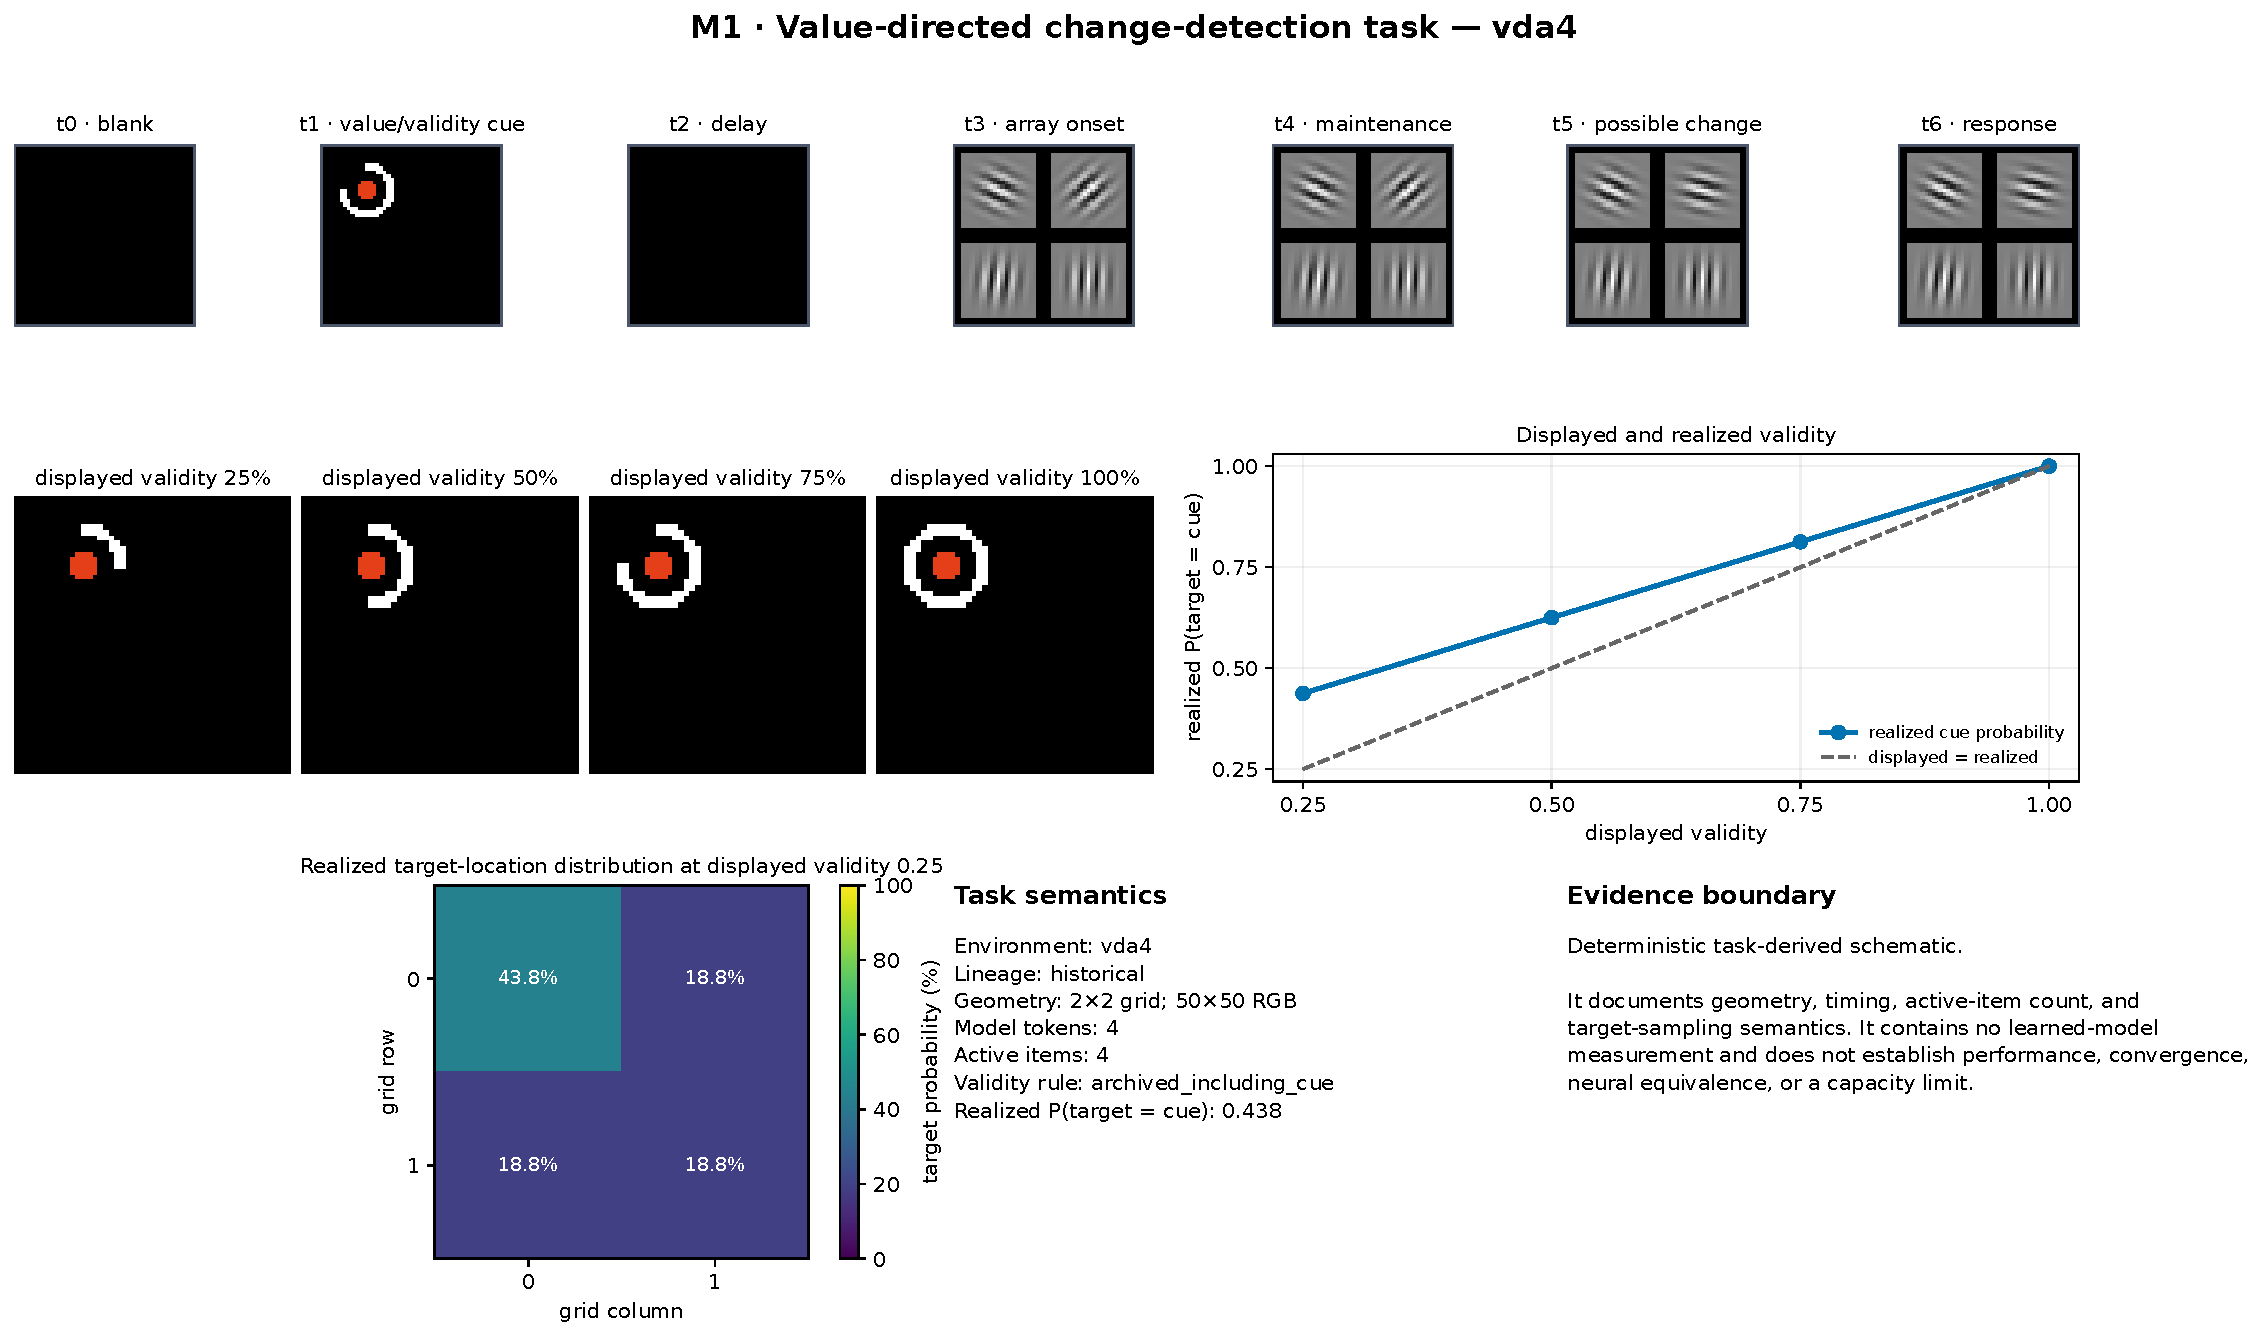
\includegraphics[width=\linewidth]{m1_task_vda4.pdf}
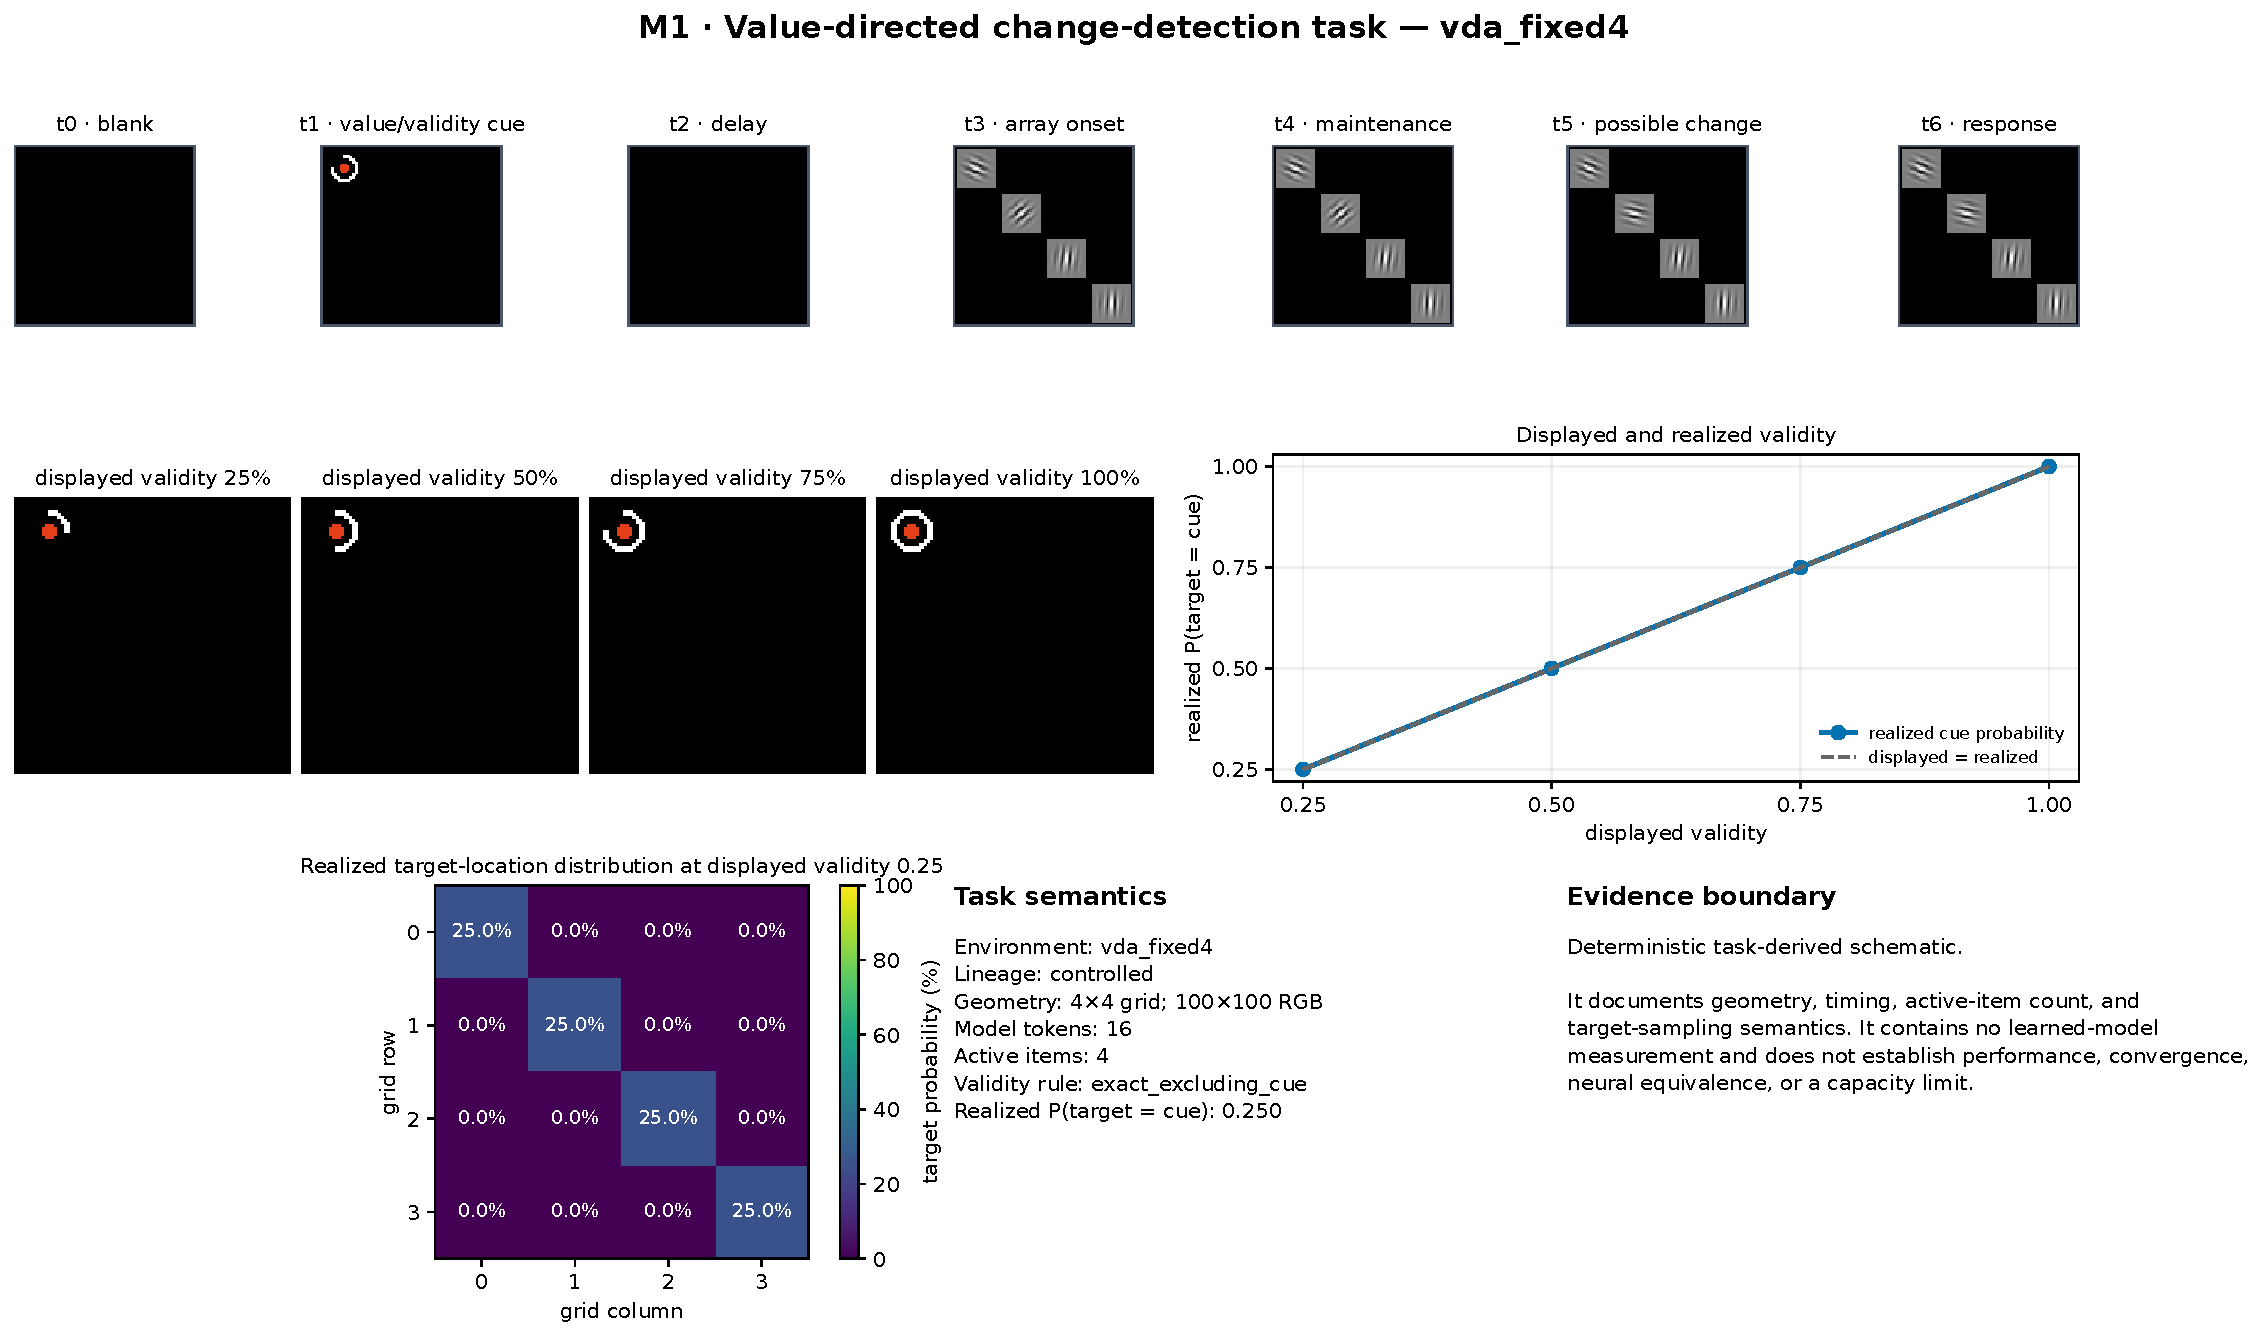
\includegraphics[width=\linewidth]{m1_task_vda_fixed4.pdf}
\caption{\textbf{Historical (top) and controlled fixed-grid (bottom) four-item task specifications.} Deterministic task schematics; seven-frame sequence, geometry, and validity semantics are specified, not measured.}\label{fig:m1-task}
\end{figure}

\subsection{Recurrent architecture}\label{sec:architecture}
The shared pipeline (Figure~\ref{fig:m2-arch}A) converts each frame to spatial patch tokens, routes them through a memory-conditioned attention operator, updates a shared spatial recurrent memory, and reads the flattened state out through actor and critic heads. Two routing families are compared throughout this paper. In \env{affine\_ew} (Figure~\ref{fig:m2-arch}B), memory generates element-wise scale $\gamma$ and shift $\beta$ applied before self-attention, $X'=\gamma\odot X+\beta$. In \env{crossattn1} (Figure~\ref{fig:m2-arch}C), current visual tokens provide queries while visual and recurrent-memory streams jointly provide keys and values, so cross-attention exposes twice as many spatial keys as affine routing for the same token count. Both routers expose the same additive key-logit hook: any attention score can be biased at any chosen spatial key before the softmax, independent of the trial itself. That hook, together with the one-token-per-item design (so the attention map is a legible $N$-way array rather than a hundred-way patch grid), is what makes the causal-intervention program in Section~\ref{sec:intervention} possible on this architecture.

\begin{figure}[t]
\centering
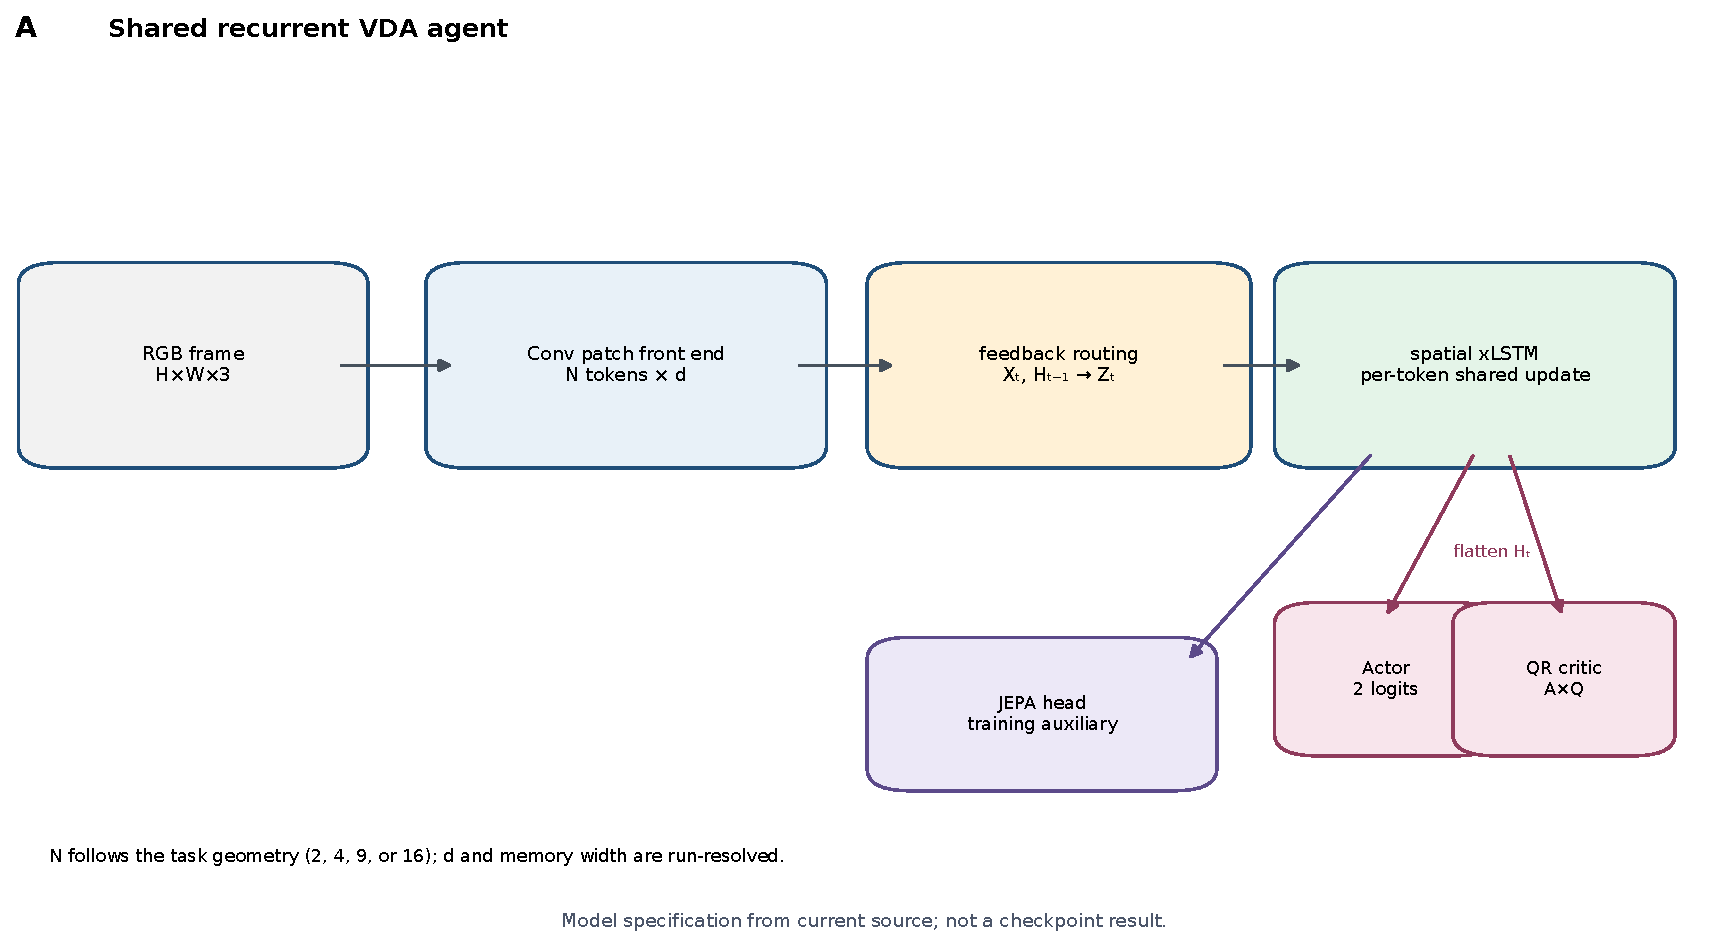
\includegraphics[width=\linewidth]{m2_architecture_a.pdf}\\[2pt]
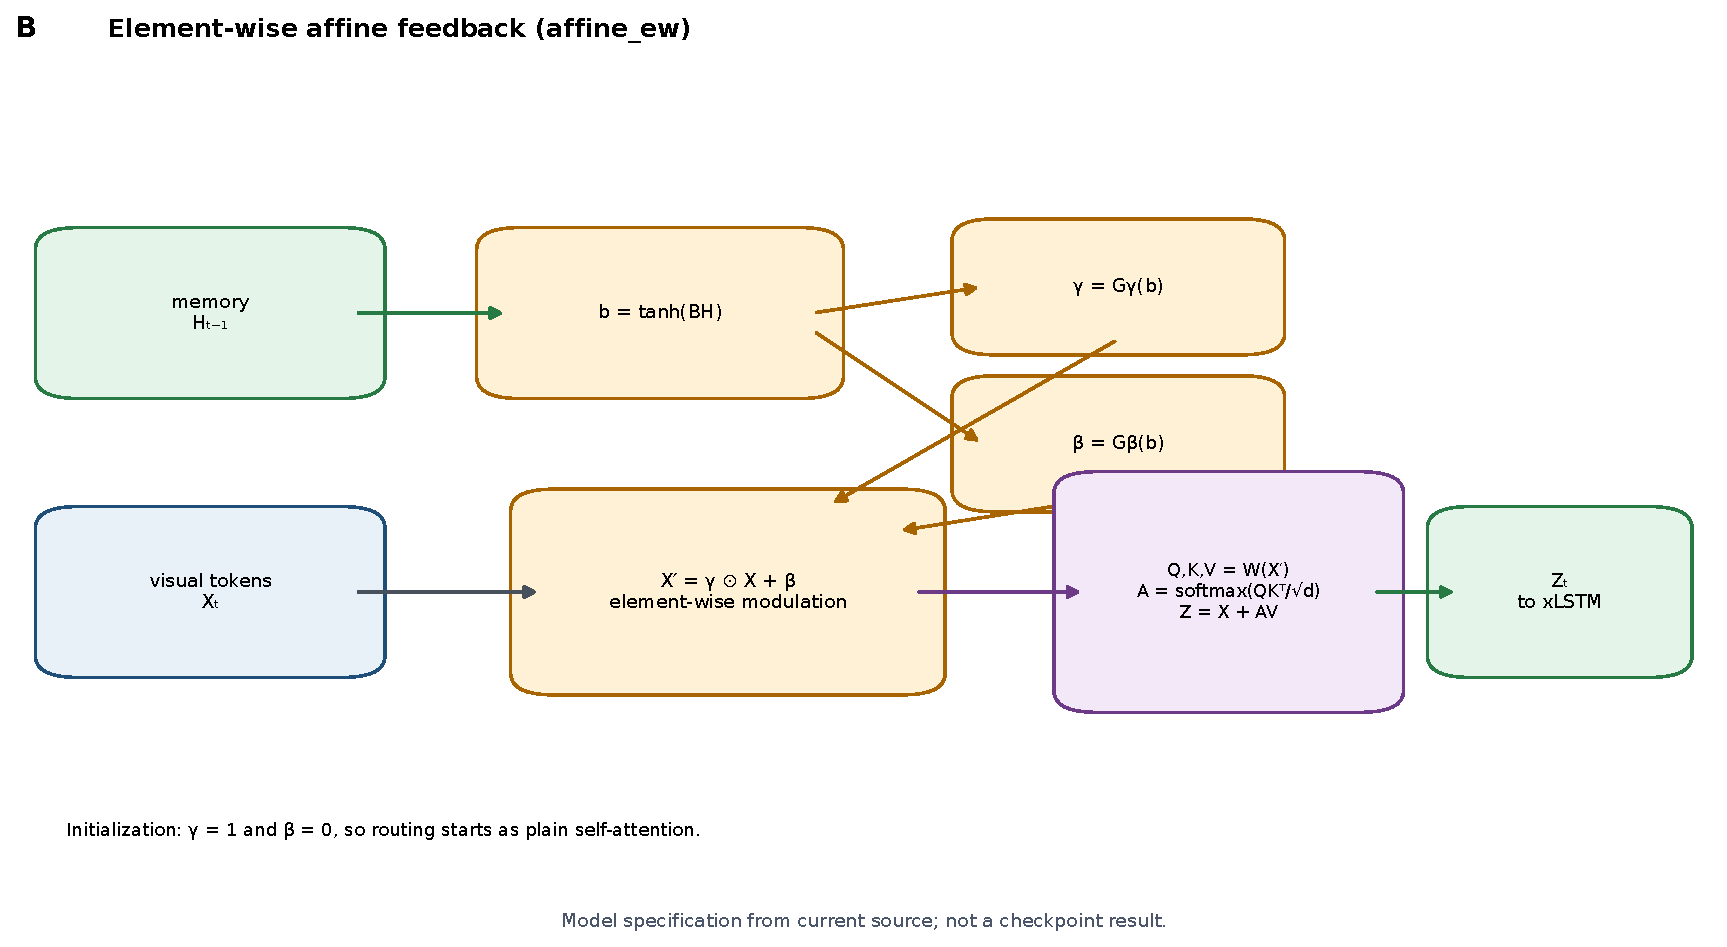
\includegraphics[width=0.49\linewidth]{m2_architecture_b.pdf}\hfill
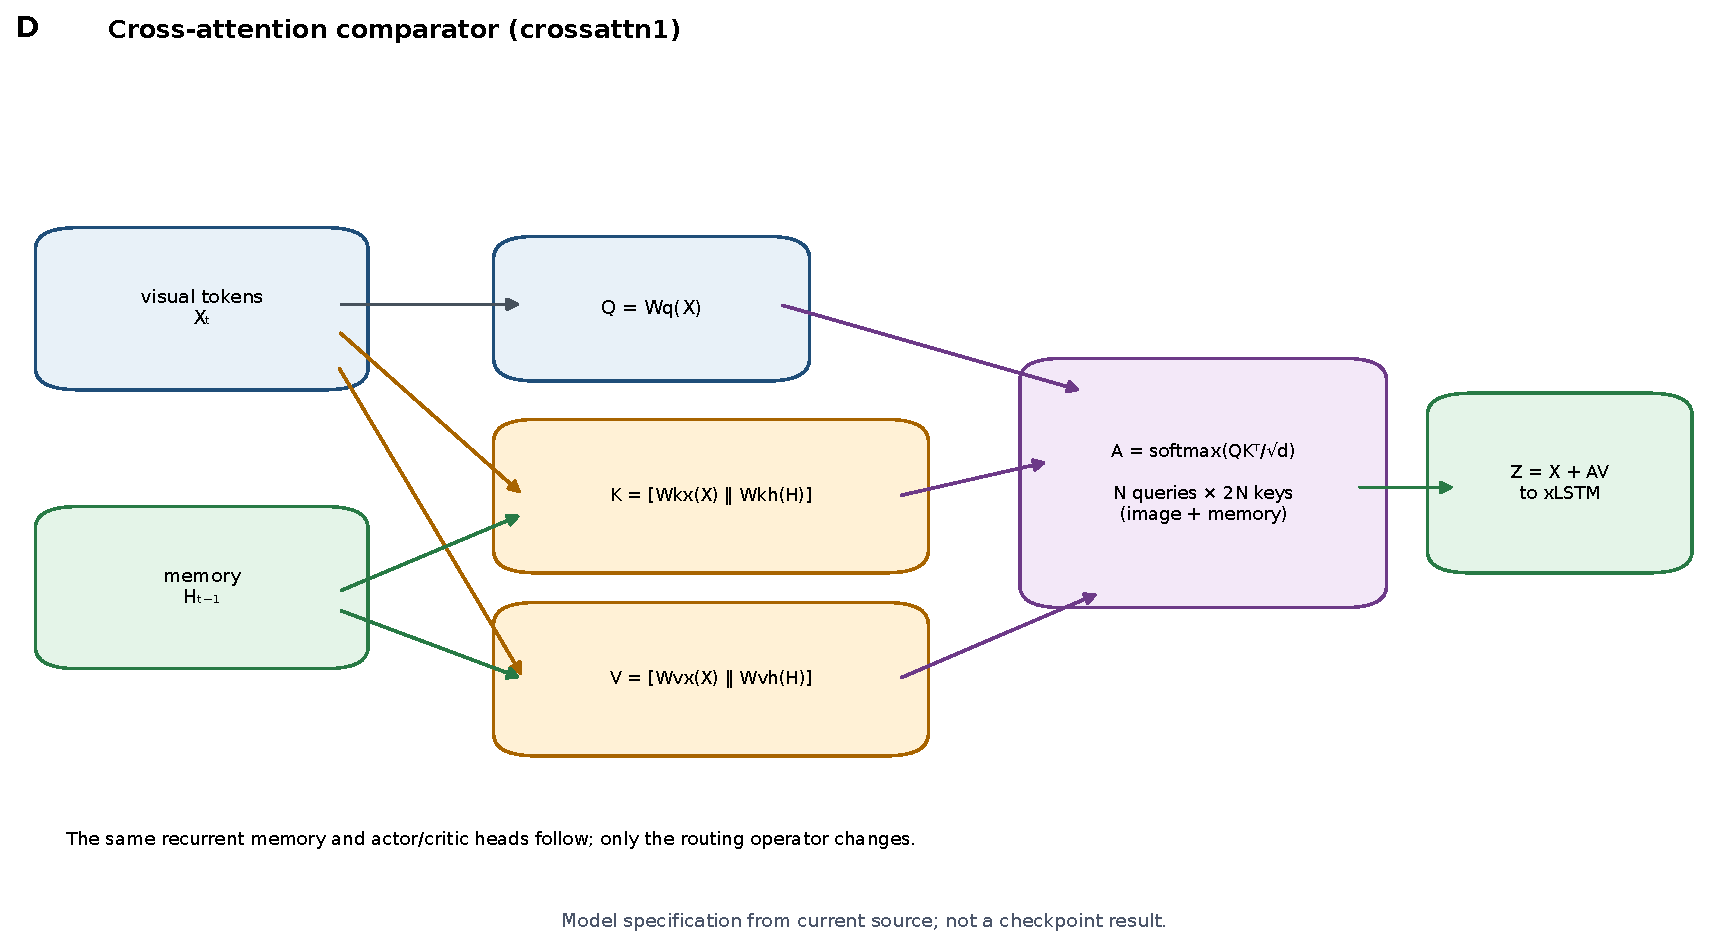
\includegraphics[width=0.49\linewidth]{m2_architecture_d.pdf}
\caption{\textbf{Architecture.} (A) Shared recurrent pipeline: patch tokens, feedback routing, spatial recurrent memory, actor/critic readout. (B) Affine element-wise feedback. (C) Cross-attention feedback: visual queries, visual+memory keys/values. Source-derived specification diagrams, not learned parameter values.}\label{fig:m2-arch}
\end{figure}

\FloatBarrier
\section{Behavioral Signatures}\label{sec:behavior}
Does the model behave like a cued observer? We answer with psychometric functions, their discrete-time chronometric counterpart, and signal detection theory wherever a criterion decomposition is available -- Carrasco's separation of discriminability from response bias, and Luo and Maunsell's demonstration that a more liberal decision policy can raise hit rate without improving sensory evidence, are the standard we hold every reported cueing effect to \cite{carrasco2011,luo2018}. We build the case from the broadest, lowest-rigor evidence to the narrowest and most controlled, because the same qualitative pattern appears at every tier and the strength of our claim should track the strength of the evidence behind it.

\subsection{A qualitative landscape across the historical ladder}
An aggregate cache spanning set sizes 1, 2, 4, and 9 and both routing families shows the qualitative signature everywhere it can be tested: change-response probability rises and response latency falls with orientation-change magnitude, and, where an uncued comparison is defined, cued responses generally lead uncued ones (Figure~\ref{fig:m3-overview}). \note{This cache carries no producer hash, per-point trial count, or uncertainty interval, and VDA1 has no uncued comparator by construction (a singleton is always cued) -- it establishes a qualitative landscape, not a quantitative one.}

\begin{figure}[t]
\centering
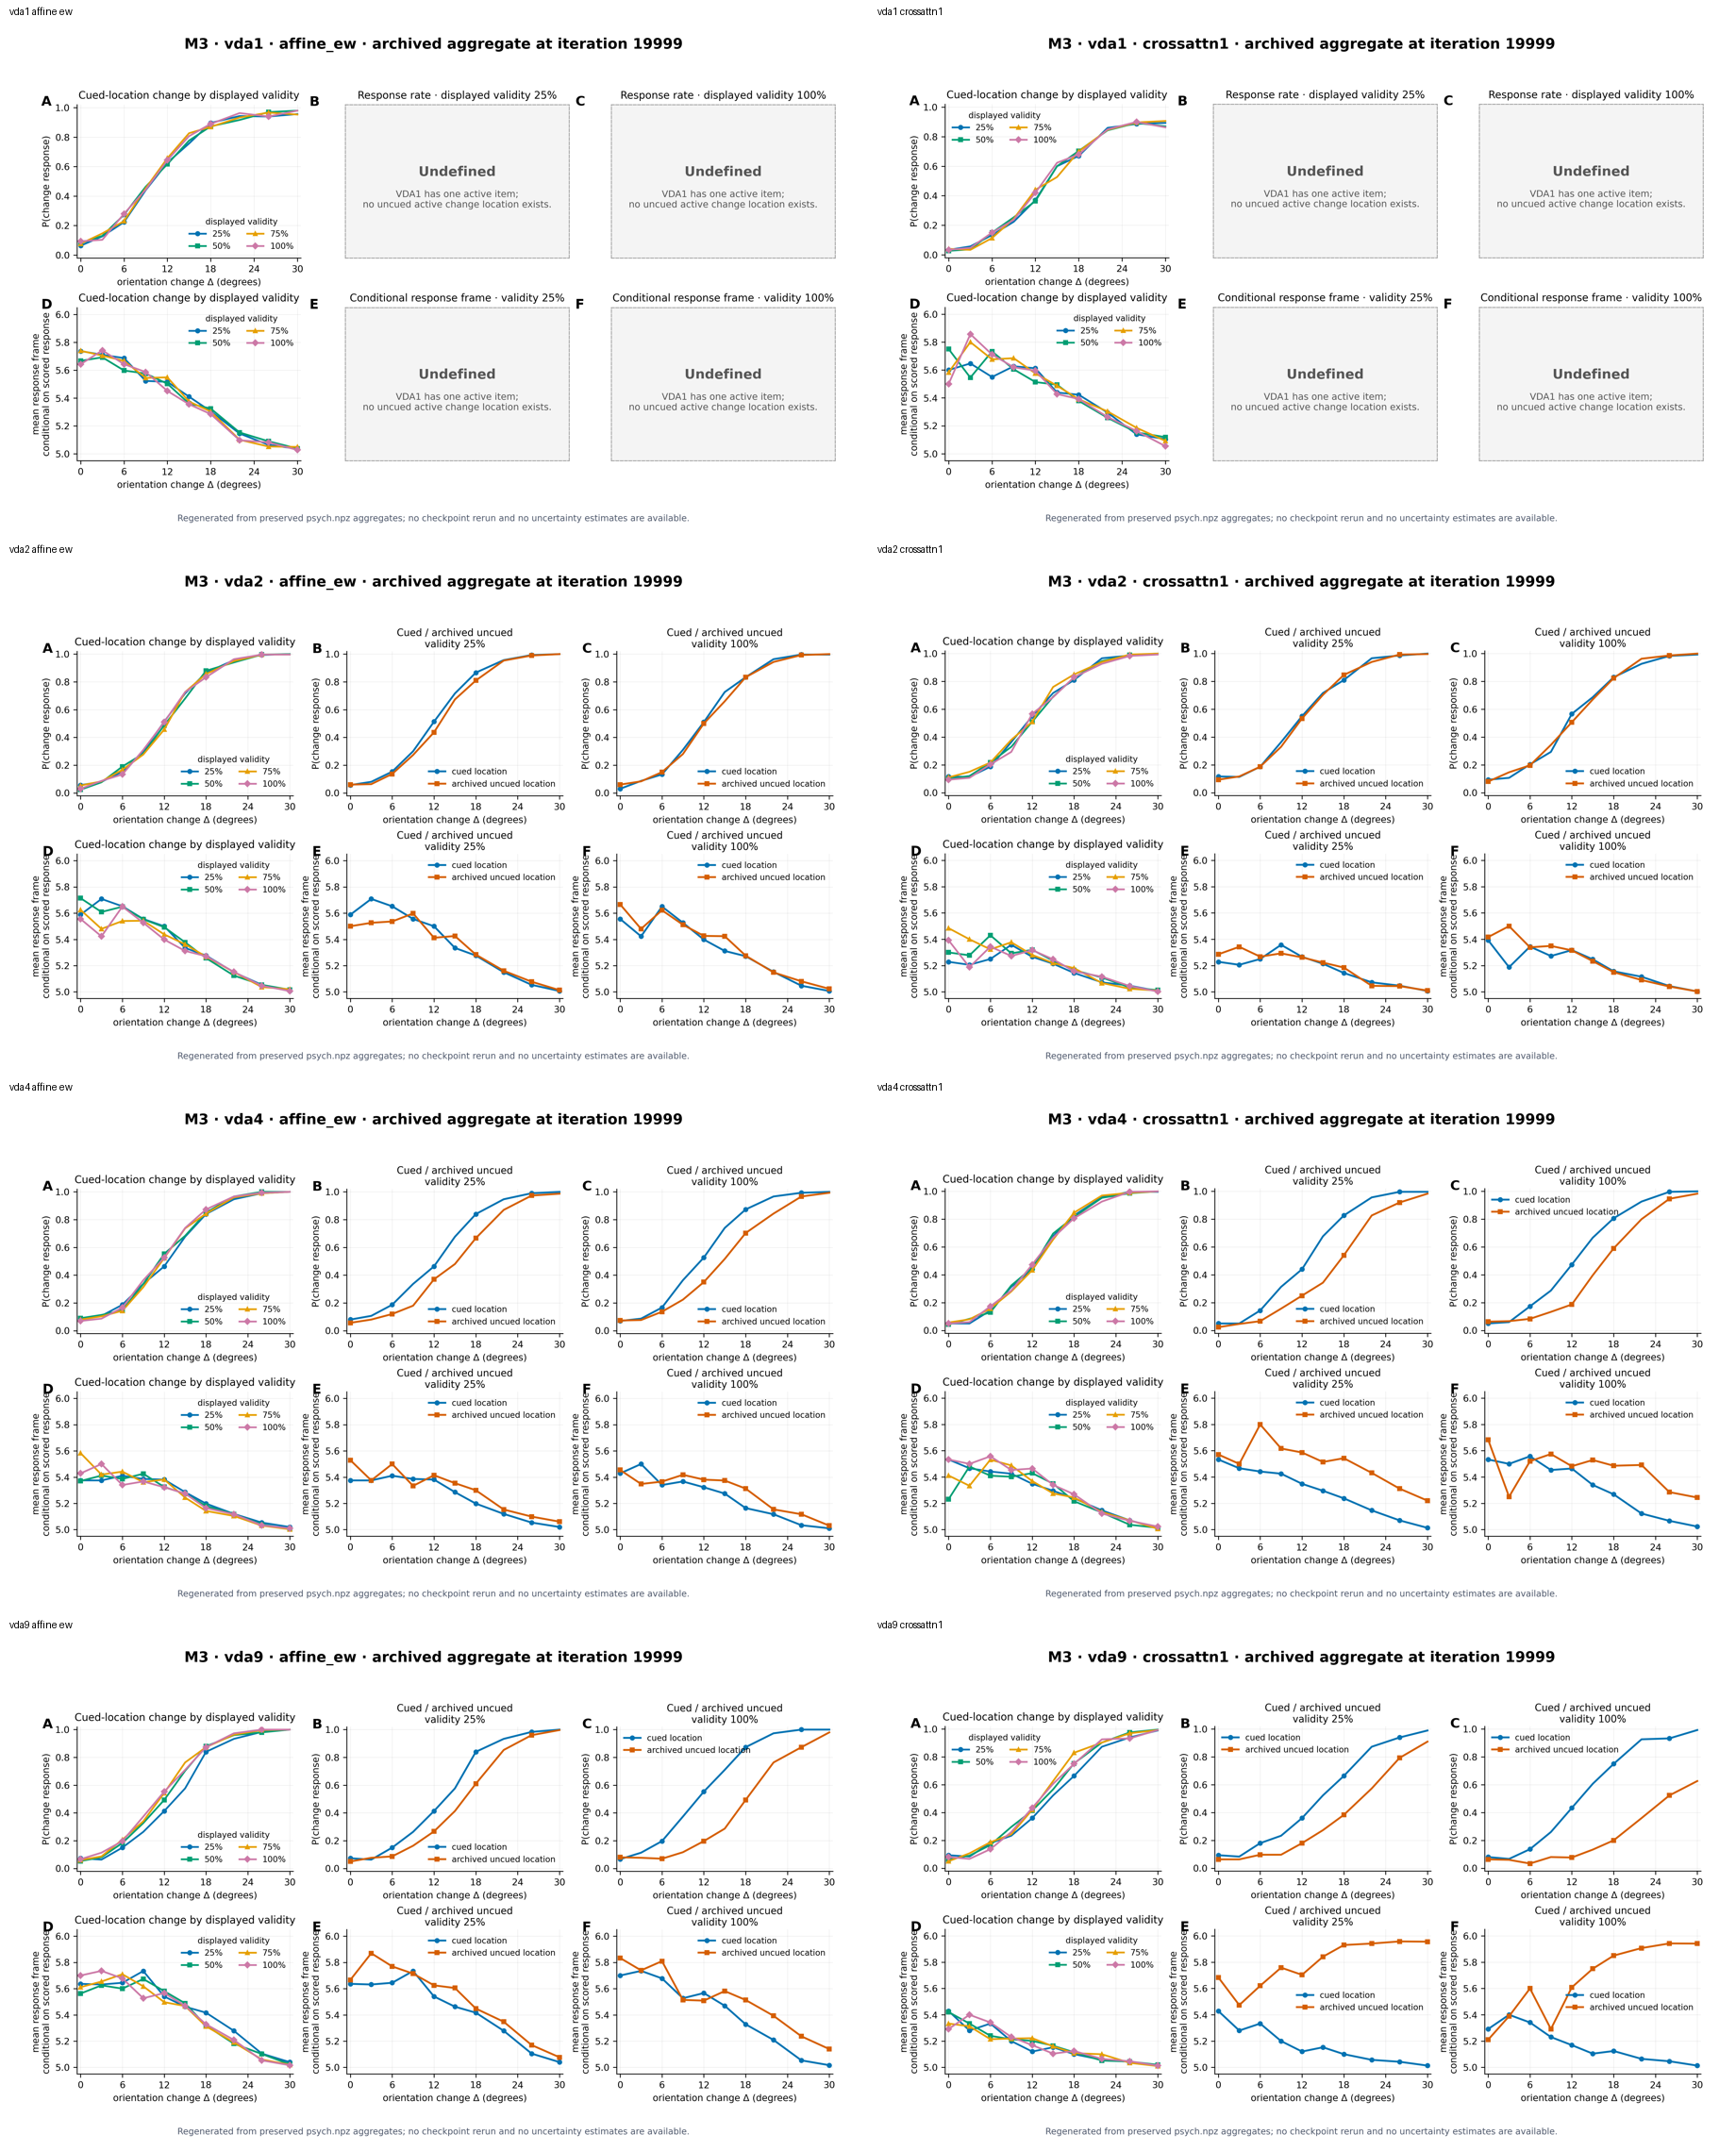
\includegraphics[width=\linewidth]{m3_behavior_contact_sheet.png}
\caption{\textbf{Cueing looks behaviorally real across the historical ladder.} Rows: VDA1, VDA2, VDA4, VDA9; columns: affine then cross-attention. A--C response probability, D--F conditional response frame. Regenerated from a preserved aggregate archive; checkpoints not rerun.}\label{fig:m3-overview}
\end{figure}

\subsection{Checkpoint-verified psychometrics at set sizes 4 and 9}\label{sec:first-wave-behavior}
A separate, provenance-closed recomputation executes one iteration-19{,}999 checkpoint per task--routing pair directly (VDA4 and VDA9, both routing families), fixing the cue at S1 and sweeping displayed cue proportion while forcing the change to the cued location or a fixed opposite location (S4 or S9). Three hundred trials back every point. Change-response probability rises with orientation change in every checkpoint, and fixed-cued estimates exceed fixed-opposite estimates at intermediate magnitudes (Figure~\ref{fig:first-wave-psych}).

\begin{figure*}[t]
\centering
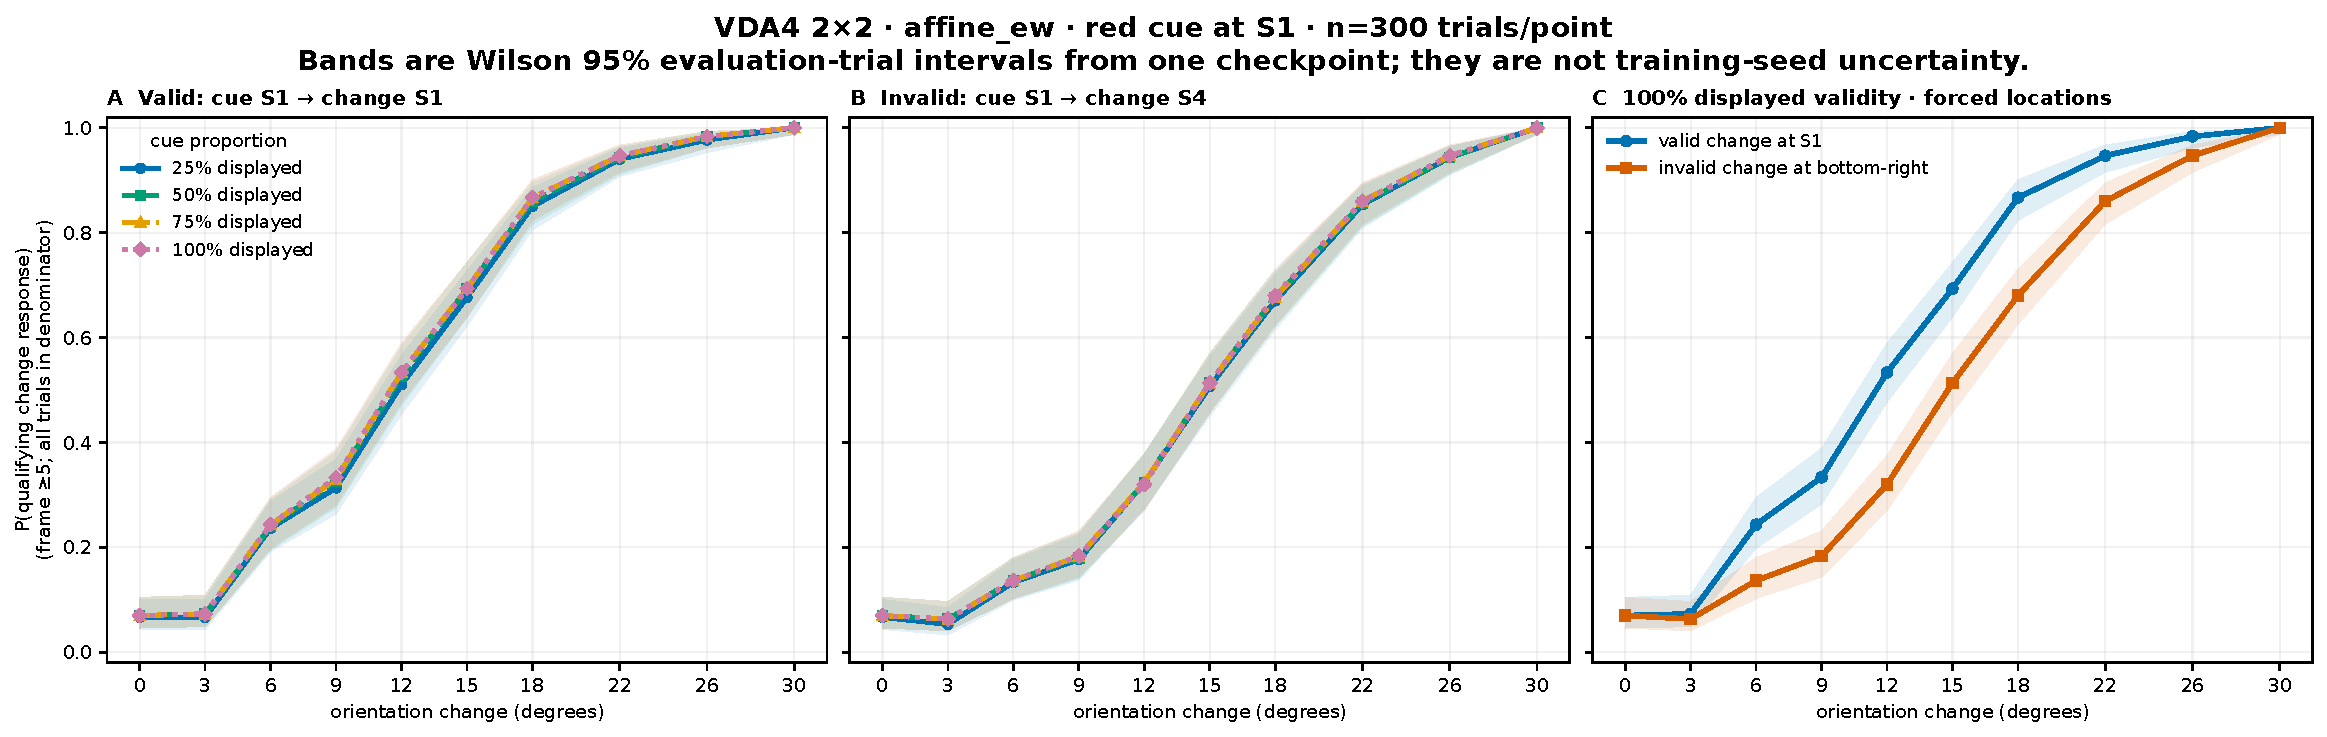
\includegraphics[width=0.49\textwidth]{first_wave_psychometric_vda4_affine_ew.pdf}\hfill
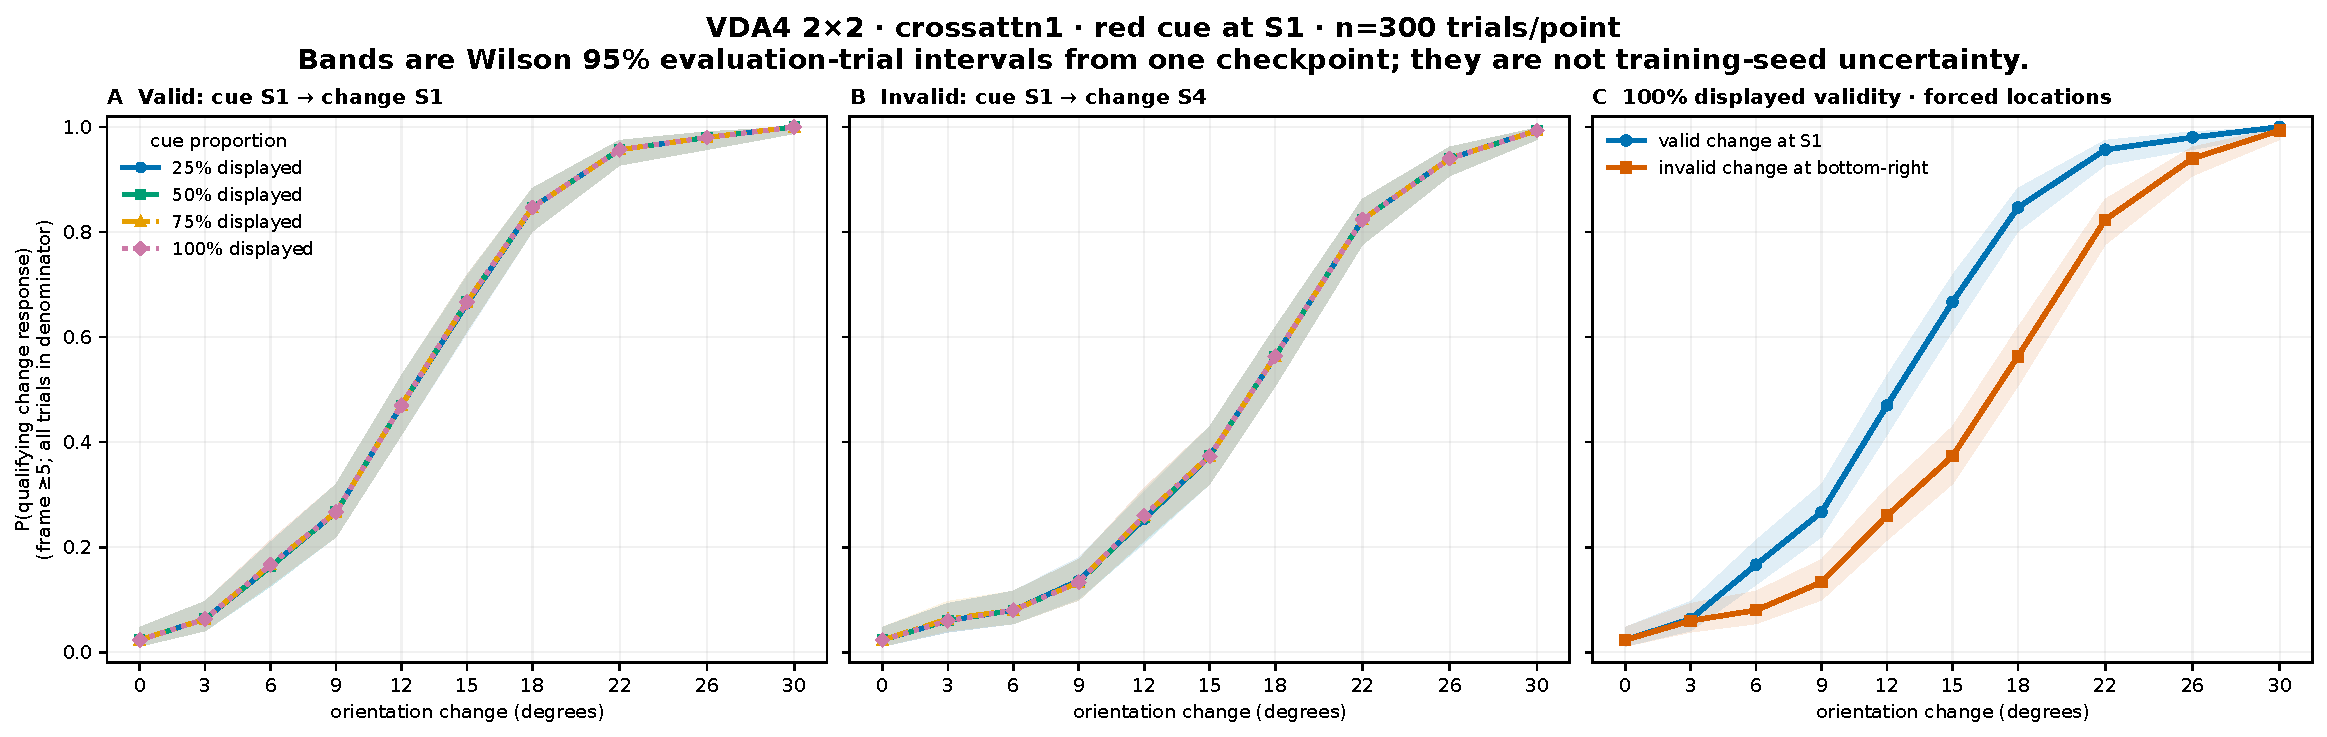
\includegraphics[width=0.49\textwidth]{first_wave_psychometric_vda4_crossattn1.pdf}\\[4pt]
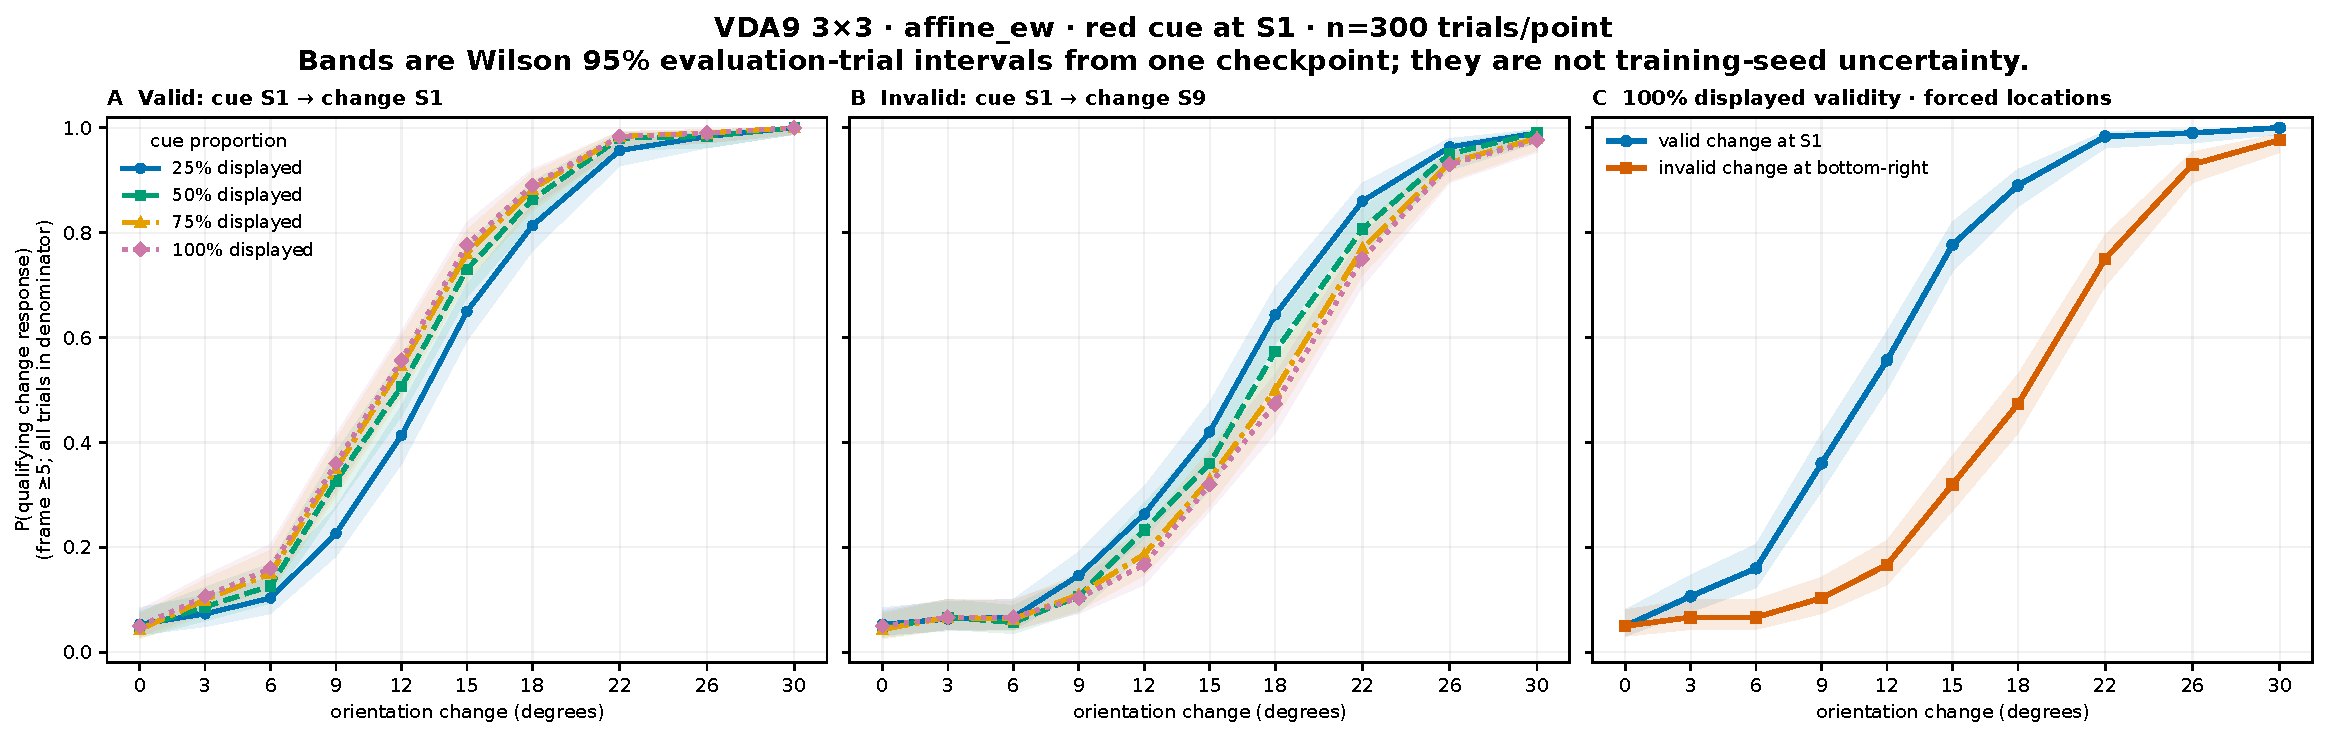
\includegraphics[width=0.49\textwidth]{first_wave_psychometric_vda9_affine_ew.pdf}\hfill
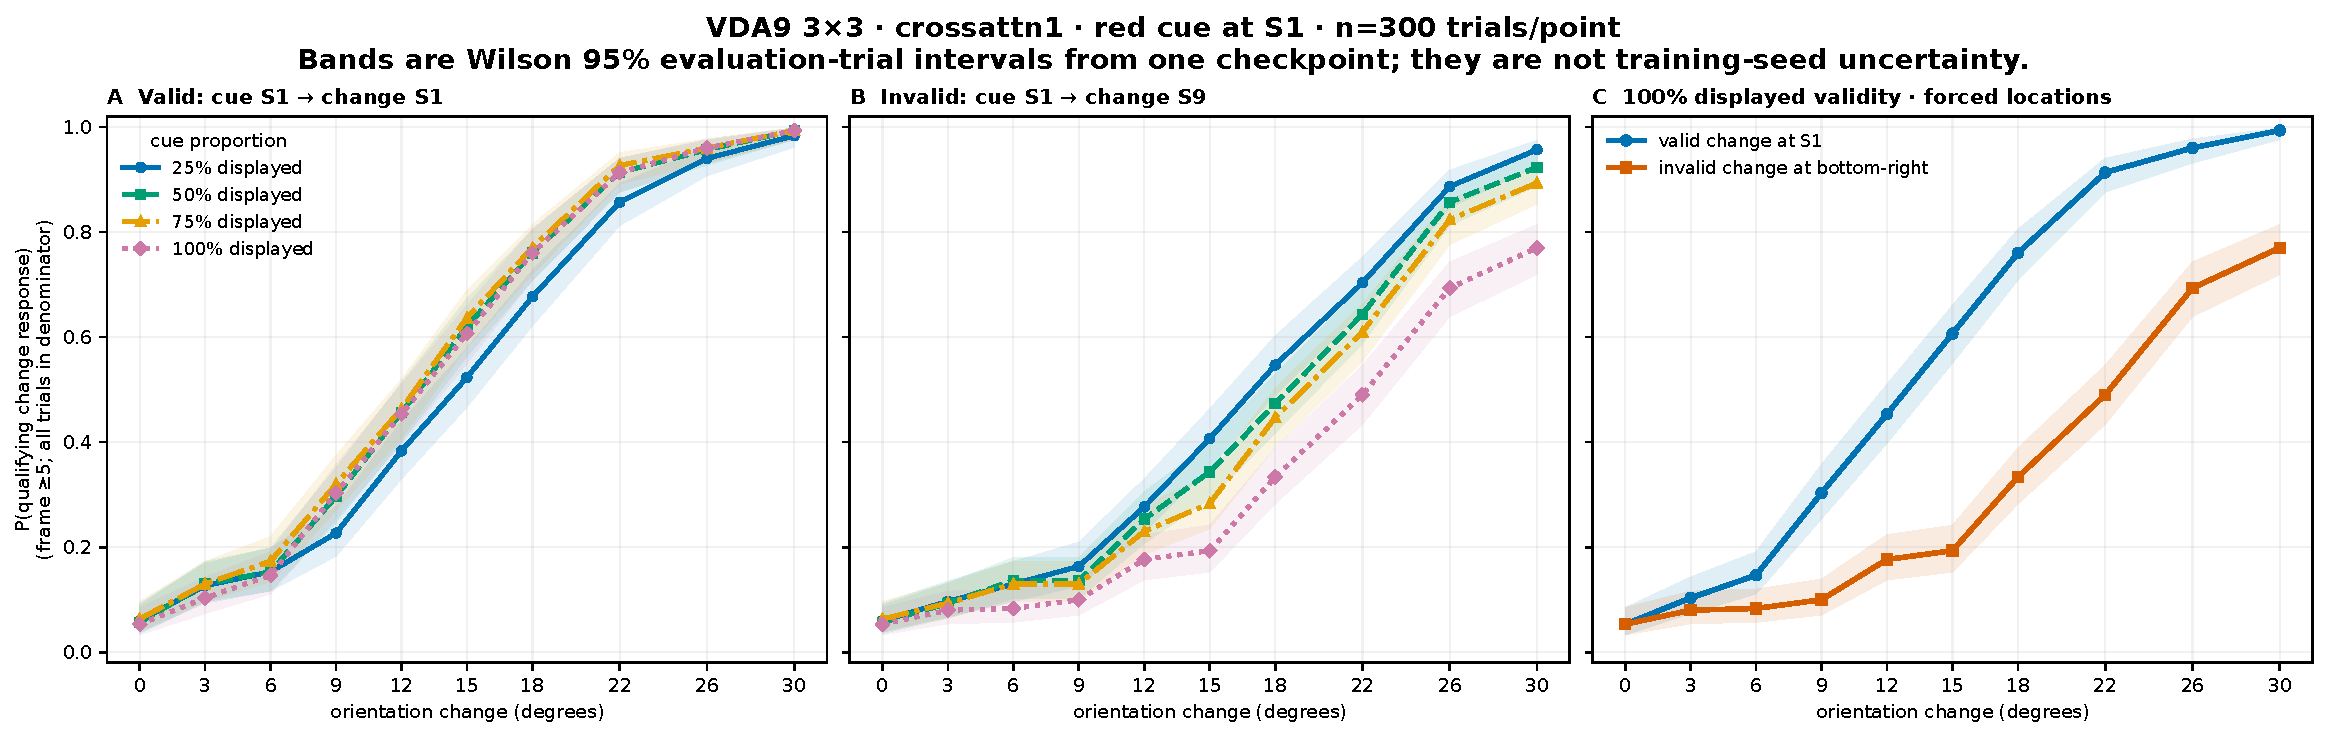
\includegraphics[width=0.49\textwidth]{first_wave_psychometric_vda9_crossattn1.pdf}
\caption{\textbf{Checkpoint-recomputed psychometrics, 300 trials/point, Wilson 95\% intervals.} Top: VDA4, affine (left) and cross-attention (right). Bottom: VDA9. Panels A/B fix the change at the cued or opposite location while sweeping displayed cue proportion; Panel C re-plots their 100\%-displayed endpoints.}\label{fig:first-wave-psych}
\end{figure*}

\subsection{Does recurrent width change the cueing benefit?}\label{sec:width-behavior}
A matched battery pairs each first-wave checkpoint (plus VDA1) with a separately trained checkpoint carrying twice the recurrent width ($d_\mathrm{mem}=256$ vs.\ 128). Width here is a descriptive grouping contrast, not a causal manipulation -- the paired checkpoints were trained separately. At $14^\circ$, VDA1 cross-attention gains 21 percentage points going from d128 to d256, while VDA4 cross-attention \emph{loses} 13; none of the five admitted pairs share a common direction (Figure~\ref{fig:matched-width}A). \textbf{A wider recurrent state does not consistently produce a larger cueing benefit}, foreshadowing the routing-family result of Section~\ref{sec:psychometric-fits}: capacity-like manipulations of this architecture do not behave like a clean capacity law.

\begin{figure*}[t]
\centering
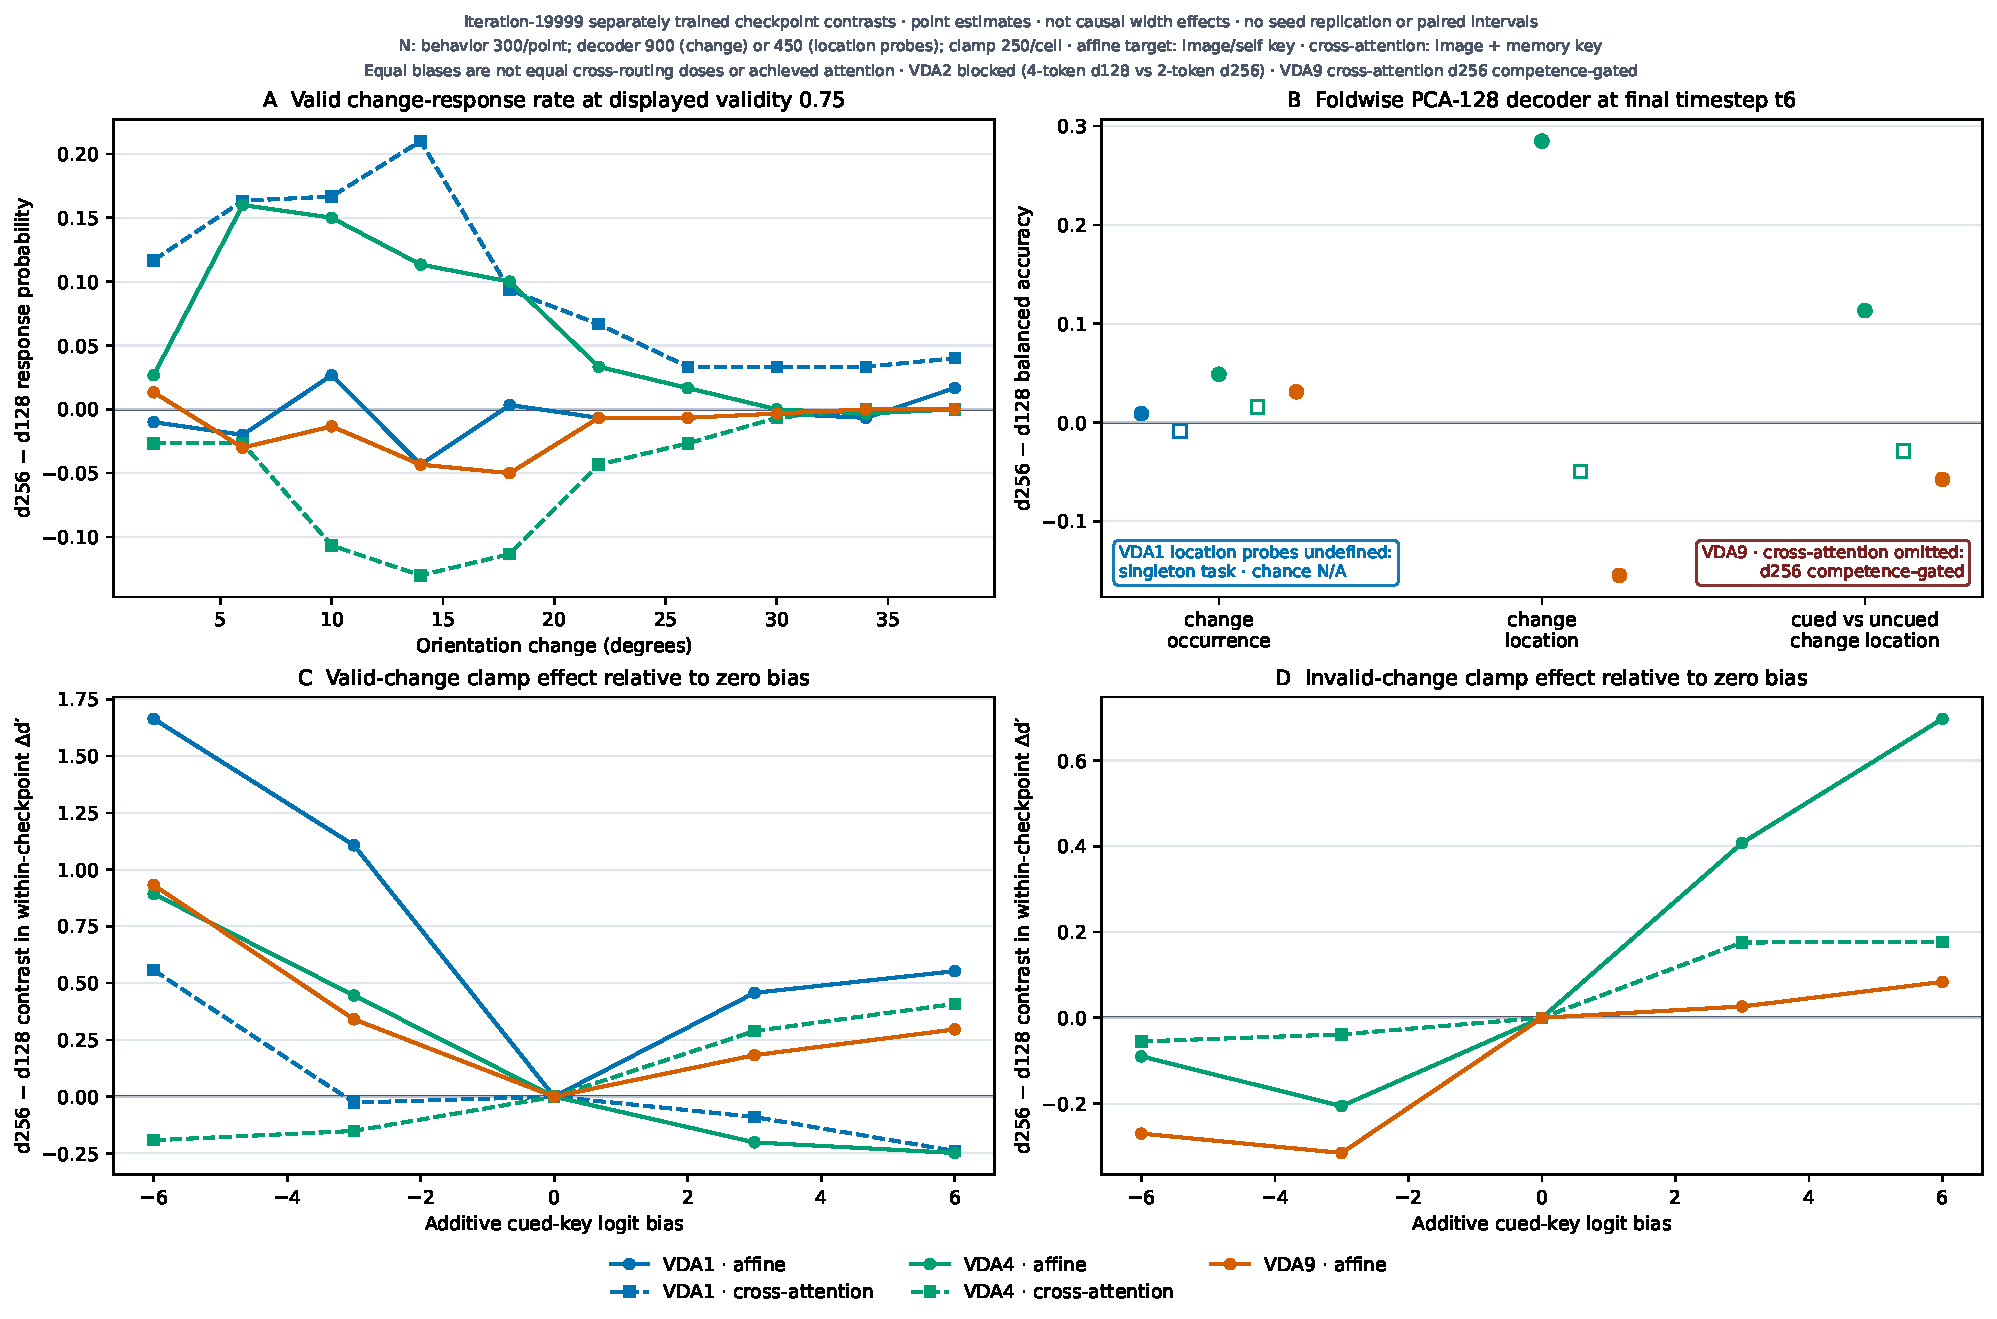
\includegraphics[width=0.85\textwidth]{matched_width_summary.pdf}
\caption{\textbf{Width does not predict the cueing benefit.} Five d256-vs-d128 checkpoint pairs, no consistent direction. (A) Valid-location response differences (behavioral). (B) t6 decoder differences (Section~\ref{sec:width-decoding}). (C--D) Within-checkpoint $d'$ change from an additive routing-key bias, compared across width (Section~\ref{sec:existing-intervention}).}\label{fig:matched-width}
\end{figure*}

\subsection{VDA16: the payoff of a larger, fully controlled set size}\label{sec:vda16-behavior}
Two controlled VDA16 checkpoints -- fixed $4\times4$ grid, sixteen tokens, $d_\mathrm{mem}=128$, seed 0, one cross-attention and one affine -- reached terminal iteration 19{,}999 and passed the VDA16 production validation gate. Neither reached the task's declared $8^\circ$ curriculum floor (cross-attention plateaued at $\theta=65^\circ$, affine advanced further to $\theta=47^\circ$ after a statefully resumed training run), so both are \emph{competence-gated} diagnostics of an easy condition rather than evidence of full convergence.

At displayed validity 0.75 and the change nearest $18^\circ$, cross-attention's qualifying response rate is \textbf{0.653 valid vs.\ 0.133 forced-invalid} ($\Delta=+0.520$); a second, independent rerun with a 100\%-valid cue and the change forced to the cued location or the opposite corner reproduces the pattern at an unambiguous ceiling: \textbf{0.983 vs.\ 0.490} at $30^\circ$ (conditional mean response frames 5.20 vs.\ 5.96). The affine checkpoint shows the same qualitative pattern with a smaller gap at the same probe -- \textbf{0.893 vs.\ 0.480} ($\Delta=+0.413$) -- but stronger final-timestep decodability of change occurrence, realized location, and cued-vs-uncued location than its cross-attention counterpart (Figure~\ref{fig:vda16-behavior}). The eight-curve overlays in Figure~\ref{fig:vda16-overlay} make the routing-family contrast vivid: affine's valid and forced-invalid curves are nearly coincident across displayed cue proportions 25--75\%, diverging only at the 100\%-displayed, fully out-of-policy stress test, whereas cross-attention shows a graded, pronounced cue-proportion dependence throughout. \note{These are separately trained, single-seed checkpoints with different achieved curricula; the routing-family contrast is descriptive.}

\begin{figure*}[t]
\centering

\includegraphics[width=0.49\textwidth]{vda16_manuscript_summary.pdf}\hfill
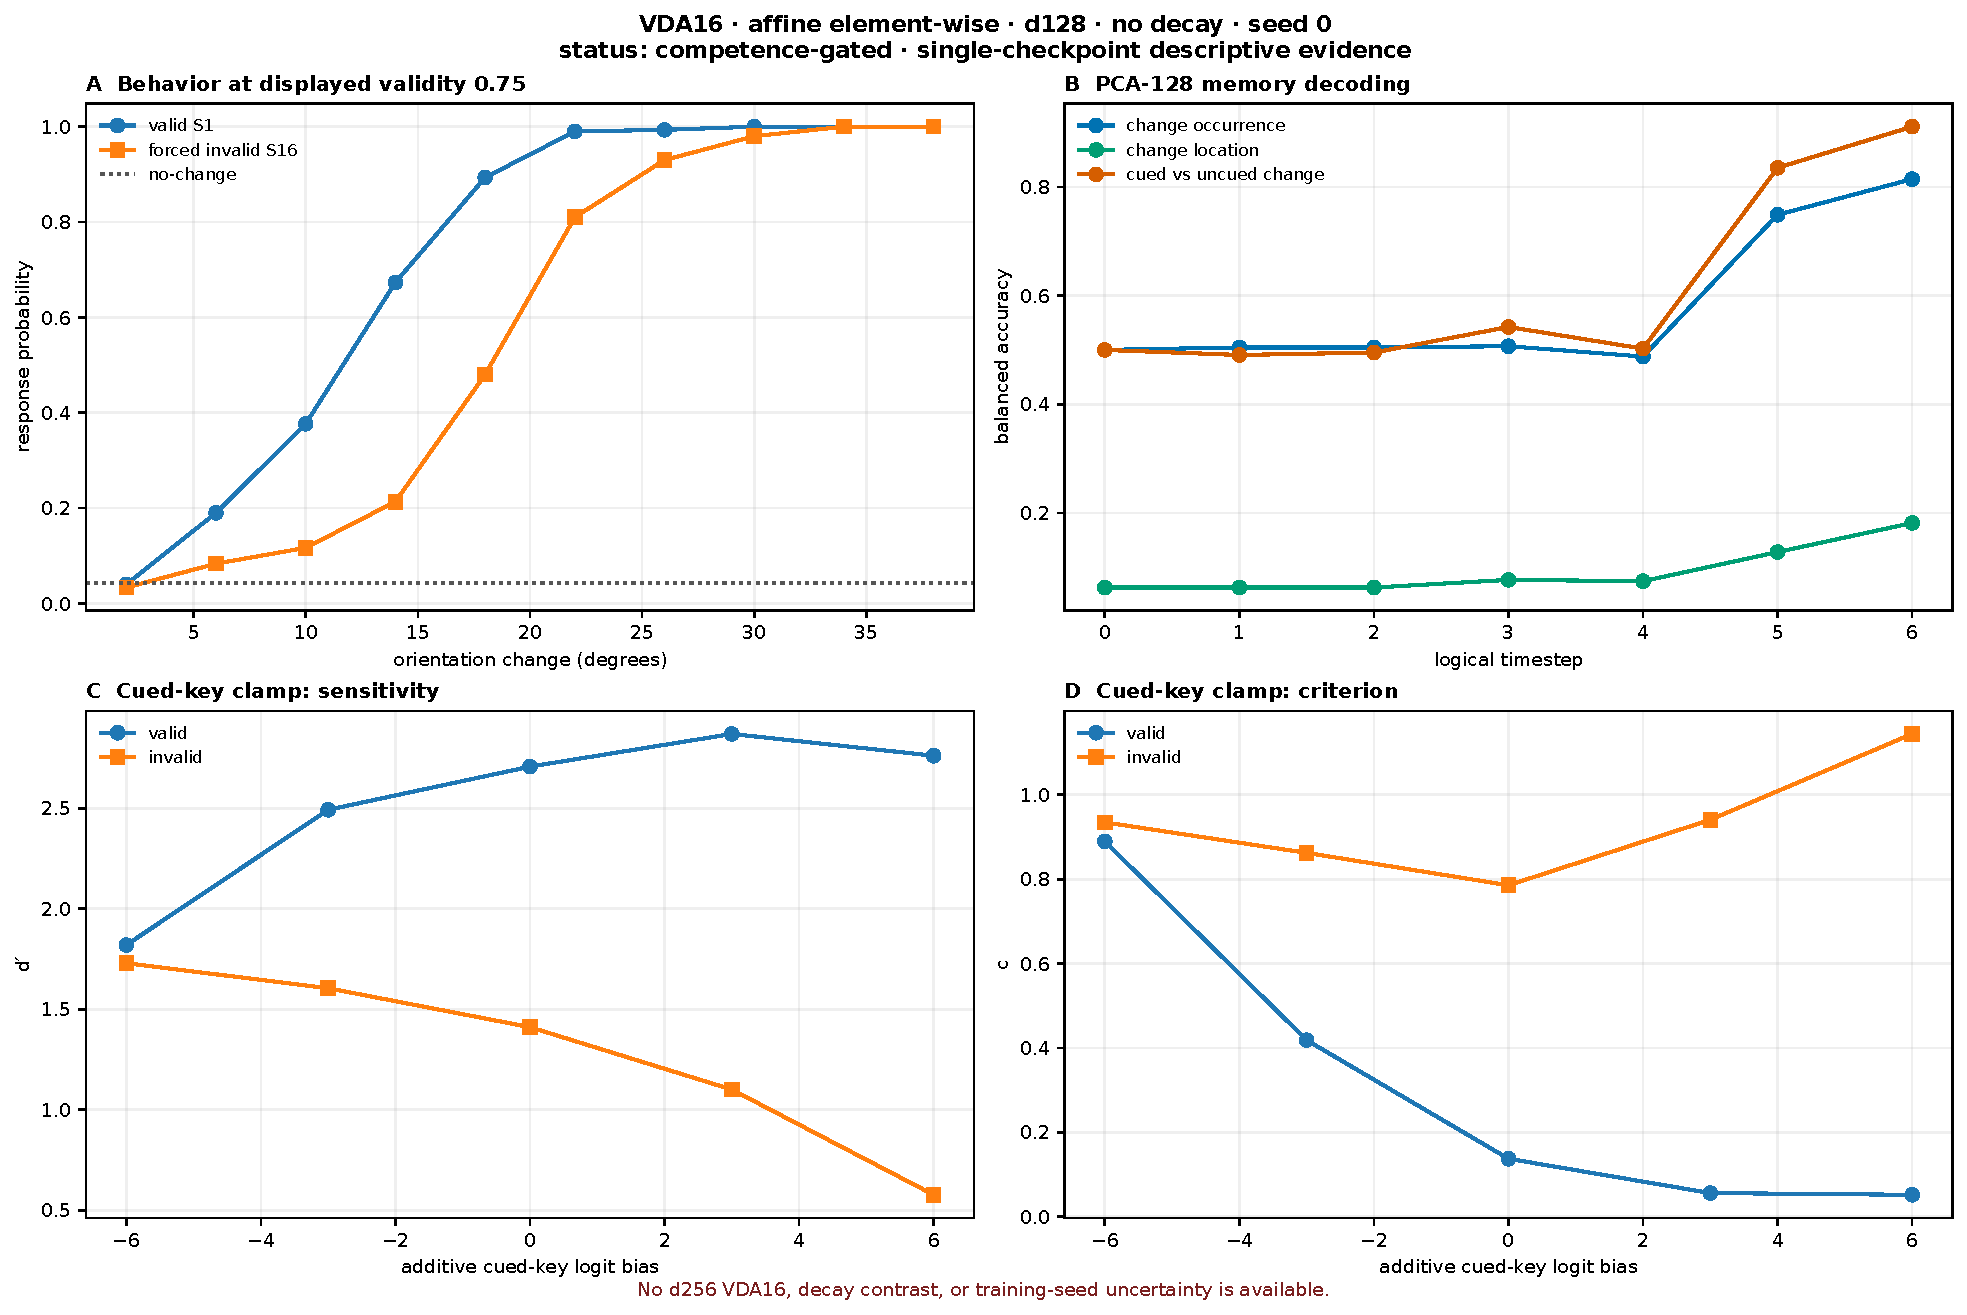
\includegraphics[width=0.49\textwidth]{vda16_affine_manuscript_summary.pdf}
\caption{\textbf{VDA16 cross-attention (left) and affine (right).} (A) Matched-bank response rates. (B) Foldwise PCA-128 decoding. (C--D) Sensitivity/criterion under additive cued-key bias (Section~\ref{sec:existing-intervention}). Both checkpoints reached iteration 19{,}999 but remain competence-gated; d256, decay-contrast, and replicated-seed cells are not admitted.}\label{fig:vda16-behavior}
\end{figure*}

\begin{figure*}[t]
\centering
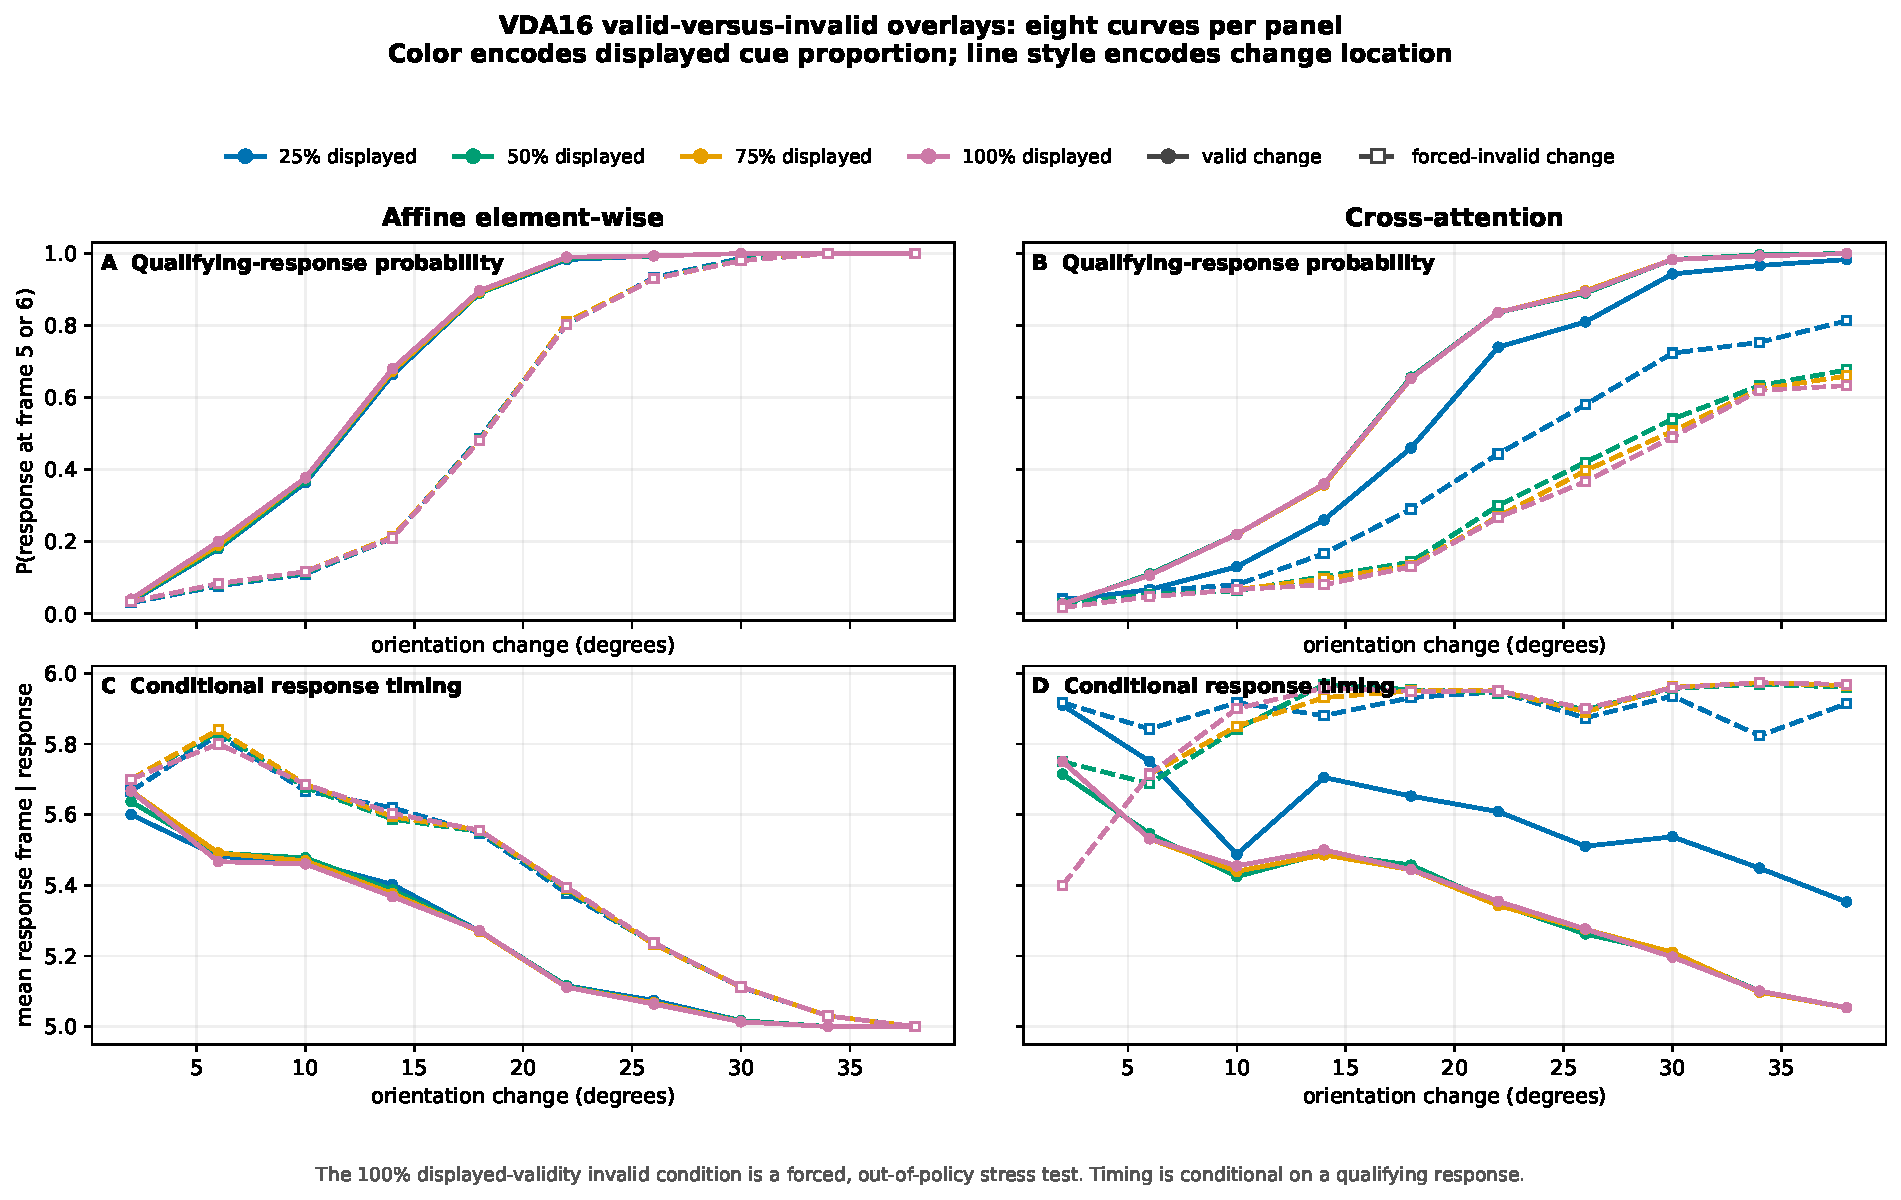
\includegraphics[width=0.85\textwidth]{vda16_valid_invalid_eight_curve_overlay.pdf}
\caption{\textbf{Affine's valid/invalid curves barely separate below 100\% displayed validity; cross-attention's separate throughout.} Four displayed cue proportions overlaid per panel, valid changes at S1 (solid) vs.\ forced-invalid changes at S16 (dashed). Top: response probability. Bottom: conditional response timing. The 100\%-displayed invalid condition is a forced, out-of-policy stress test.}\label{fig:vda16-overlay}
\end{figure*}

\subsection{Logistic psychometric functions across set size: a routing-family-specific effect}\label{sec:psychometric-fits}
To compare the cueing benefit across set size on a common scale, we fit a four-parameter logistic $p(x)=\gamma+(1-\gamma-\lambda)/(1+e^{-(x-\alpha)/\beta})$ -- threshold $\alpha$, slope $\beta$, guess rate $\gamma$, lapse rate $\lambda$ -- to the same checkpoint-recomputed arrays above (VDA4, VDA9, both routing families; both VDA16 checkpoints), a re-analysis of already-cached data with no checkpoint re-run. \textbf{The result reported in this paper's abstract lives here.} For cross-attention, the fitted threshold shift grows monotonically and roughly doubles from set size 4 to 16 ($5.3^\circ\to10.9^\circ$; Figure~\ref{fig:psych-fit}, left and center). For affine, the shift grows from set size 4 to 9 ($3.4^\circ\to6.5^\circ$) and then is essentially flat into set size 16 ($6.2^\circ$; Figure~\ref{fig:psych-fit}, right) -- set size 9, not 16, is affine's largest cueing benefit. The raw response-probability gap near $18^\circ$ tells the same story (Figure~\ref{fig:psych-fit-summary}): cross-attention grows monotonically (0.27, 0.32, 0.44 across set sizes 4/9/16) while affine rises then plateaus-to-falls (0.19, 0.38, 0.32).

\textbf{The growing-cueing-gap-with-set-size pattern that motivates this paper therefore holds cleanly within the cross-attention lineage and not within the affine lineage}, trained on the identical task. Set size is at least as much a property of which routing family is asked as it is a universal law -- a routing-family analogue of Section~\ref{sec:width-behavior}'s finding that width does not consistently predict the cueing benefit either. \note{Historical VDA4/VDA9 and controlled VDA16 differ in grid geometry and training/runtime lineage in addition to active-item count, and each point is one checkpoint, not an independent-seed population; Section~\ref{sec:discussion} returns to the specific confound between set size and spatial discretization.}

\begin{figure*}[t]
\centering
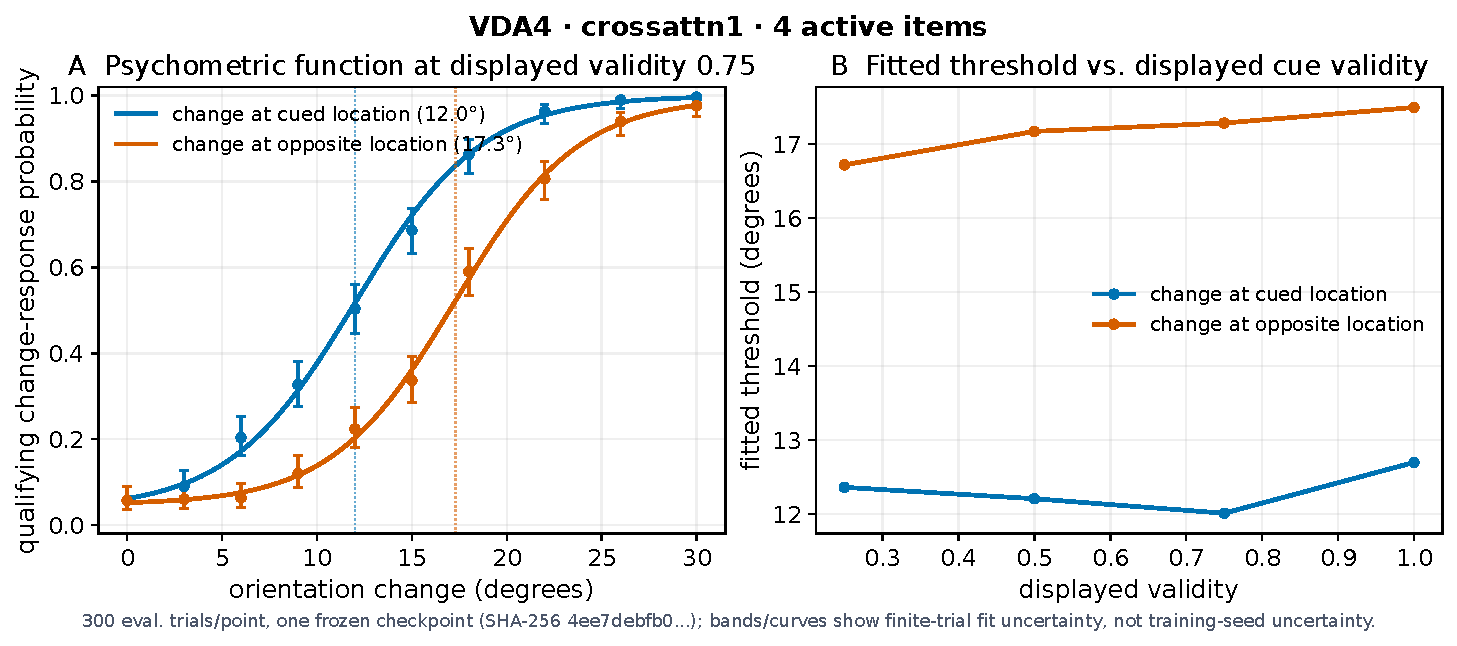
\includegraphics[width=0.485\textwidth]{psychometric_fit_vda4_crossattn1.pdf}\hfill
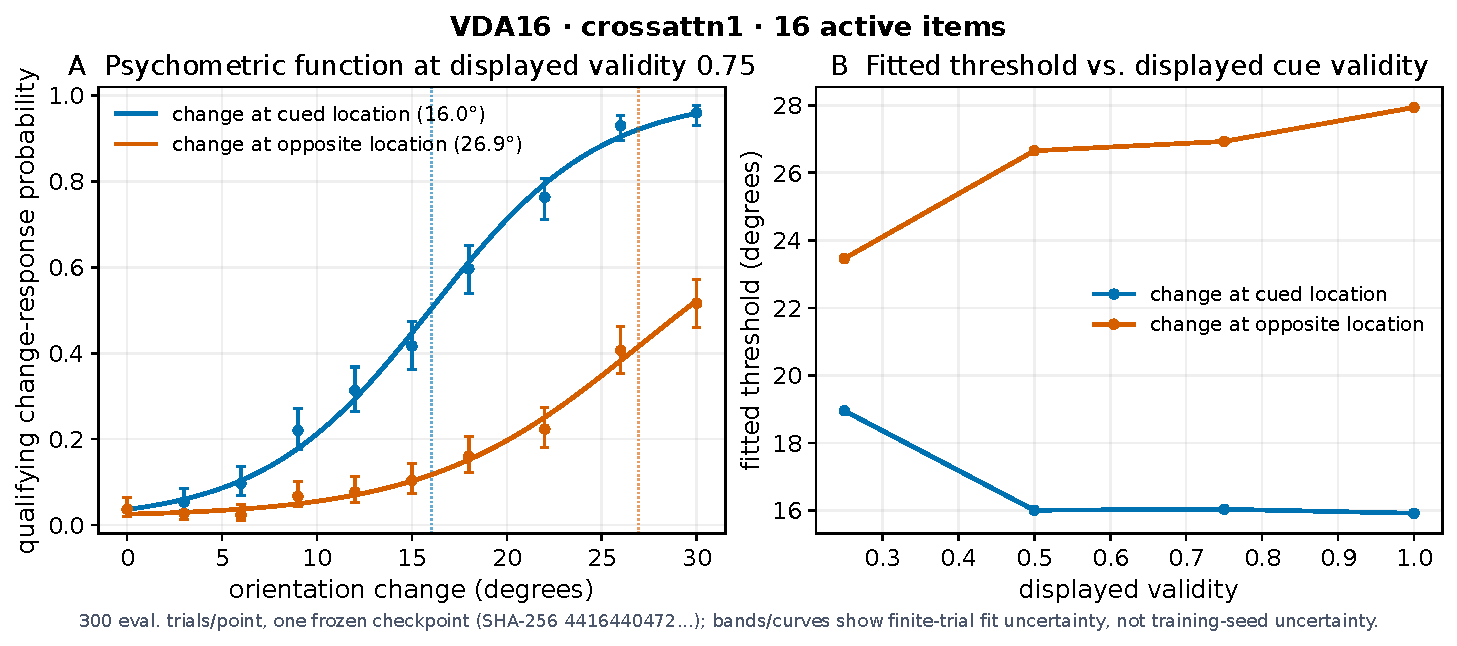
\includegraphics[width=0.485\textwidth]{psychometric_fit_vda16_crossattn1.pdf}\\[3pt]
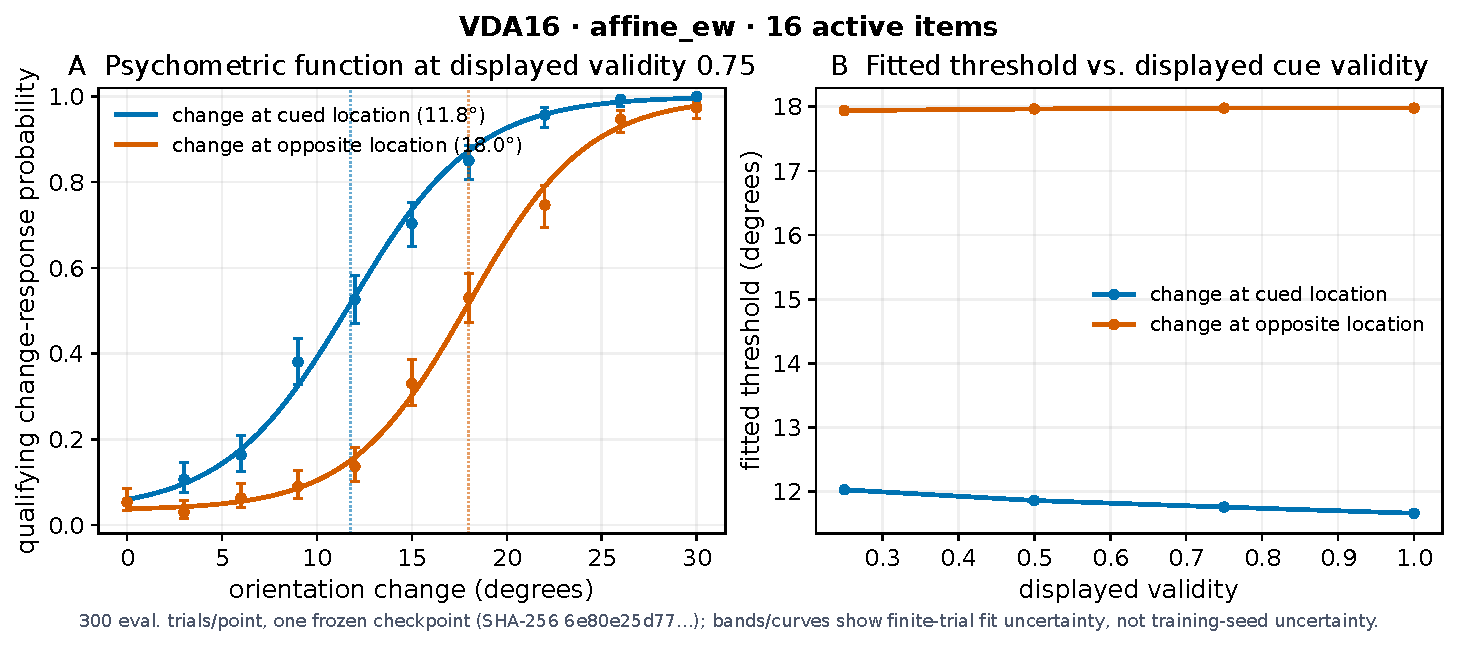
\includegraphics[width=0.485\textwidth]{psychometric_fit_vda16_affine_ew.pdf}
\caption{\textbf{Fitted psychometric functions and thresholds.} Top-left: VDA4 cross-attention (set size 4 baseline). Top-right: VDA16 cross-attention -- threshold separation roughly doubles relative to set size 4. Bottom: VDA16 affine -- separation is comparable to affine's own set-size-9 value, not double its set-size-4 value. Panel A: fitted function at displayed validity 0.75. Panel B: fitted threshold vs.\ displayed validity.}\label{fig:psych-fit}
\end{figure*}

\begin{figure}[t]
\centering
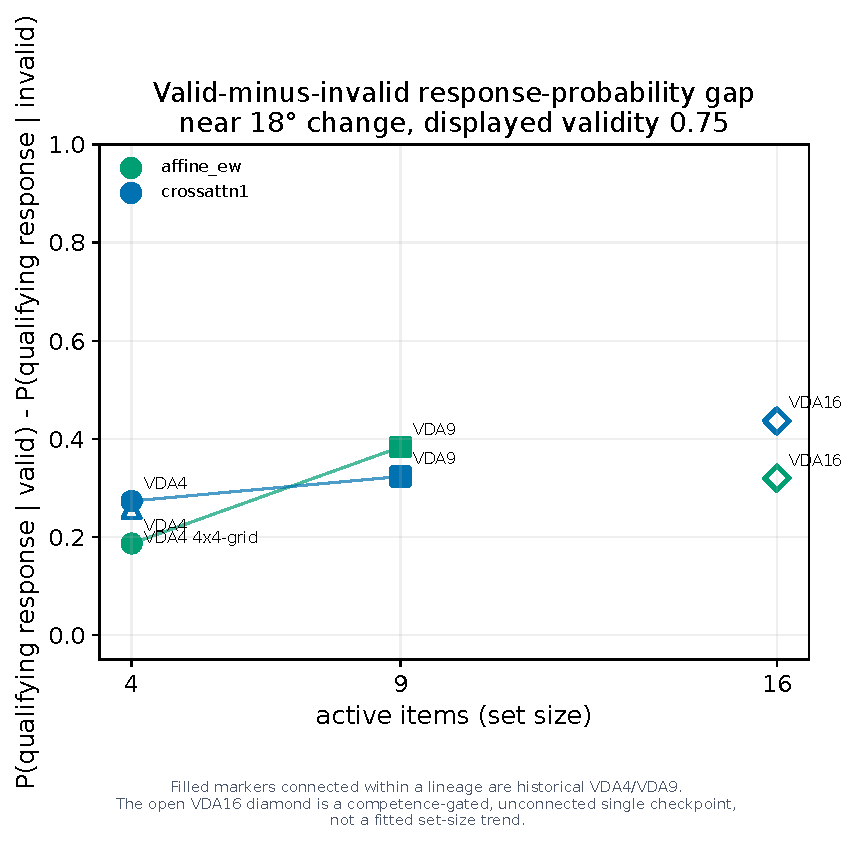
\includegraphics[width=\linewidth]{psychometric_fit_setsize_summary.pdf}
\caption{\textbf{Cueing-effect magnitude vs.\ set size, by routing family.} Valid-minus-invalid response-probability gap near $18^\circ$, displayed validity 0.75. Filled markers connected within the historical VDA4/VDA9 lineage; open VDA16 diamonds are competence-gated, differently lineaged single checkpoints plotted unconnected.}\label{fig:psych-fit-summary}
\end{figure}

\begin{figure*}[t]
\centering

\includegraphics[width=0.85\textwidth]{vda_method_comparison_with_vda16.pdf}
\caption{\textbf{Behavioral and representational context across the full set-size series.} (A) Valid-minus-invalid response rate. (B--C) Final-timestep decoders. (D) No-change false-alarm rate, which stays low and does not rise with set size -- evidence against the simplest criterion-only account of the widening gap in (A). Open VDA16 markers are competence-gated, unconnected points, not a fitted trend.}\label{fig:vda16-context}
\end{figure*}

\FloatBarrier
\section{Attention Dynamics Over Time}\label{sec:attention-dynamics}
A cueing benefit could in principle arise without the model's internal routing ever tracking the cue. This section asks where routing weight actually goes across the trial timeline -- blank, cue, delay, array, change, response -- and what a held-out linear probe can decode from the recurrent state at each point, following the same event-alignment discipline Herman and Krauzlis used to relate superior-colliculus activity to detection \cite{herman2017,carrasco2011}. Throughout, ``attention map'' names the model's own routing weights over locations, not a claim about a literal neural attention map.

\subsection{Event-aligned attention maps at set sizes 4 and 9}\label{sec:first-wave-attention}
Each map evaluates four displayed cue proportions on 96 matched no-change trials each: the cue is fixed, nothing ever changes, and t5 is retained only as the nominal change opportunity. Affine exposes one spatial-key array; cross-attention exposes separate image-key and recurrent-memory-key arrays (Figure~\ref{fig:first-wave-attn}).

\begin{figure*}[t]
\centering
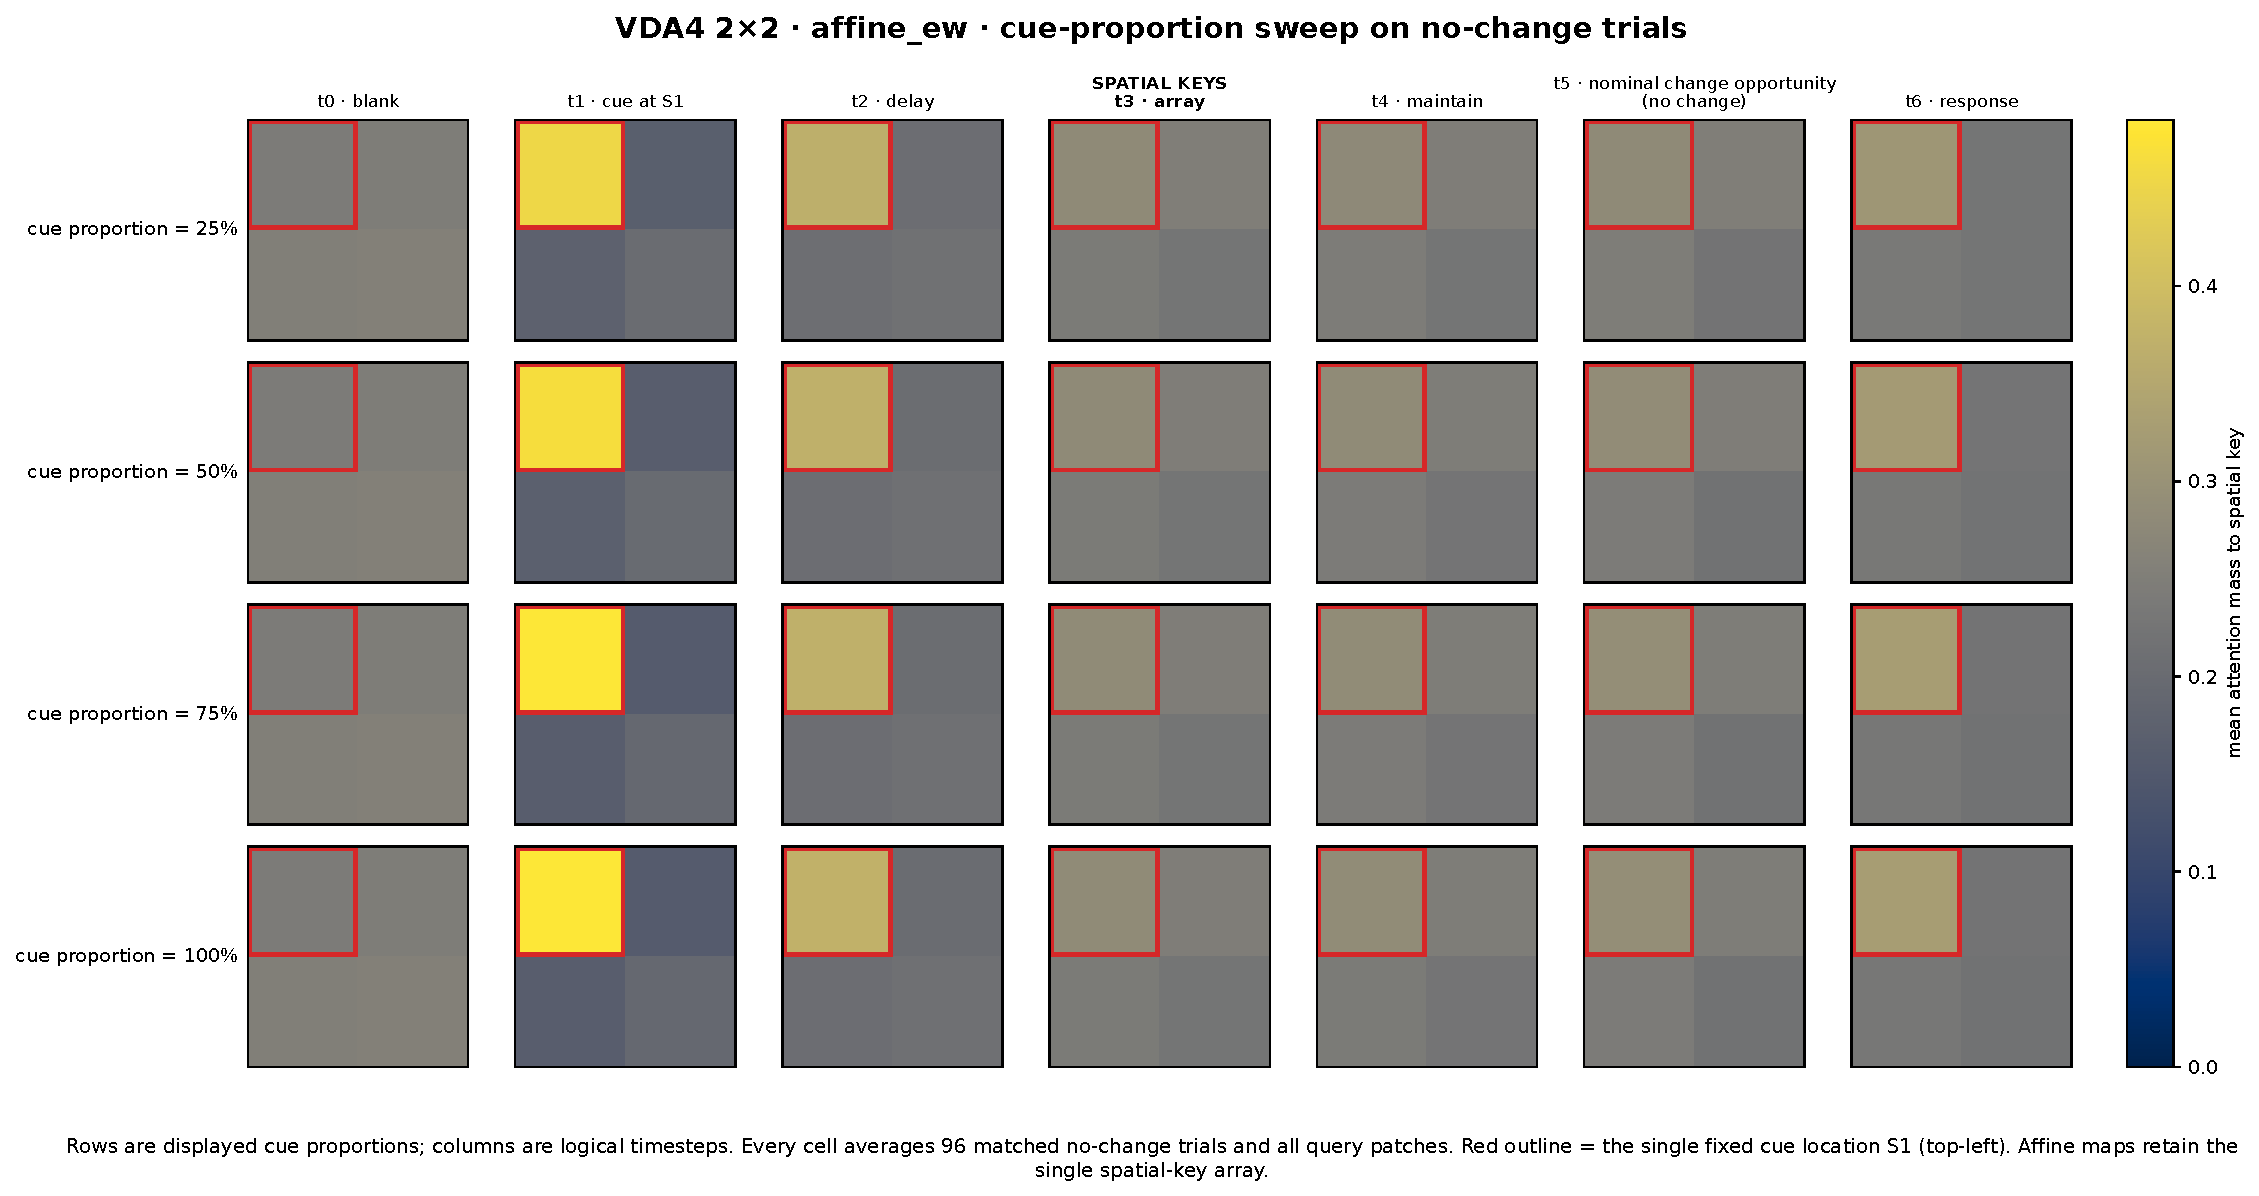
\includegraphics[width=0.32\textwidth]{first_wave_attention_vda4_affine_ew.pdf}\hfill
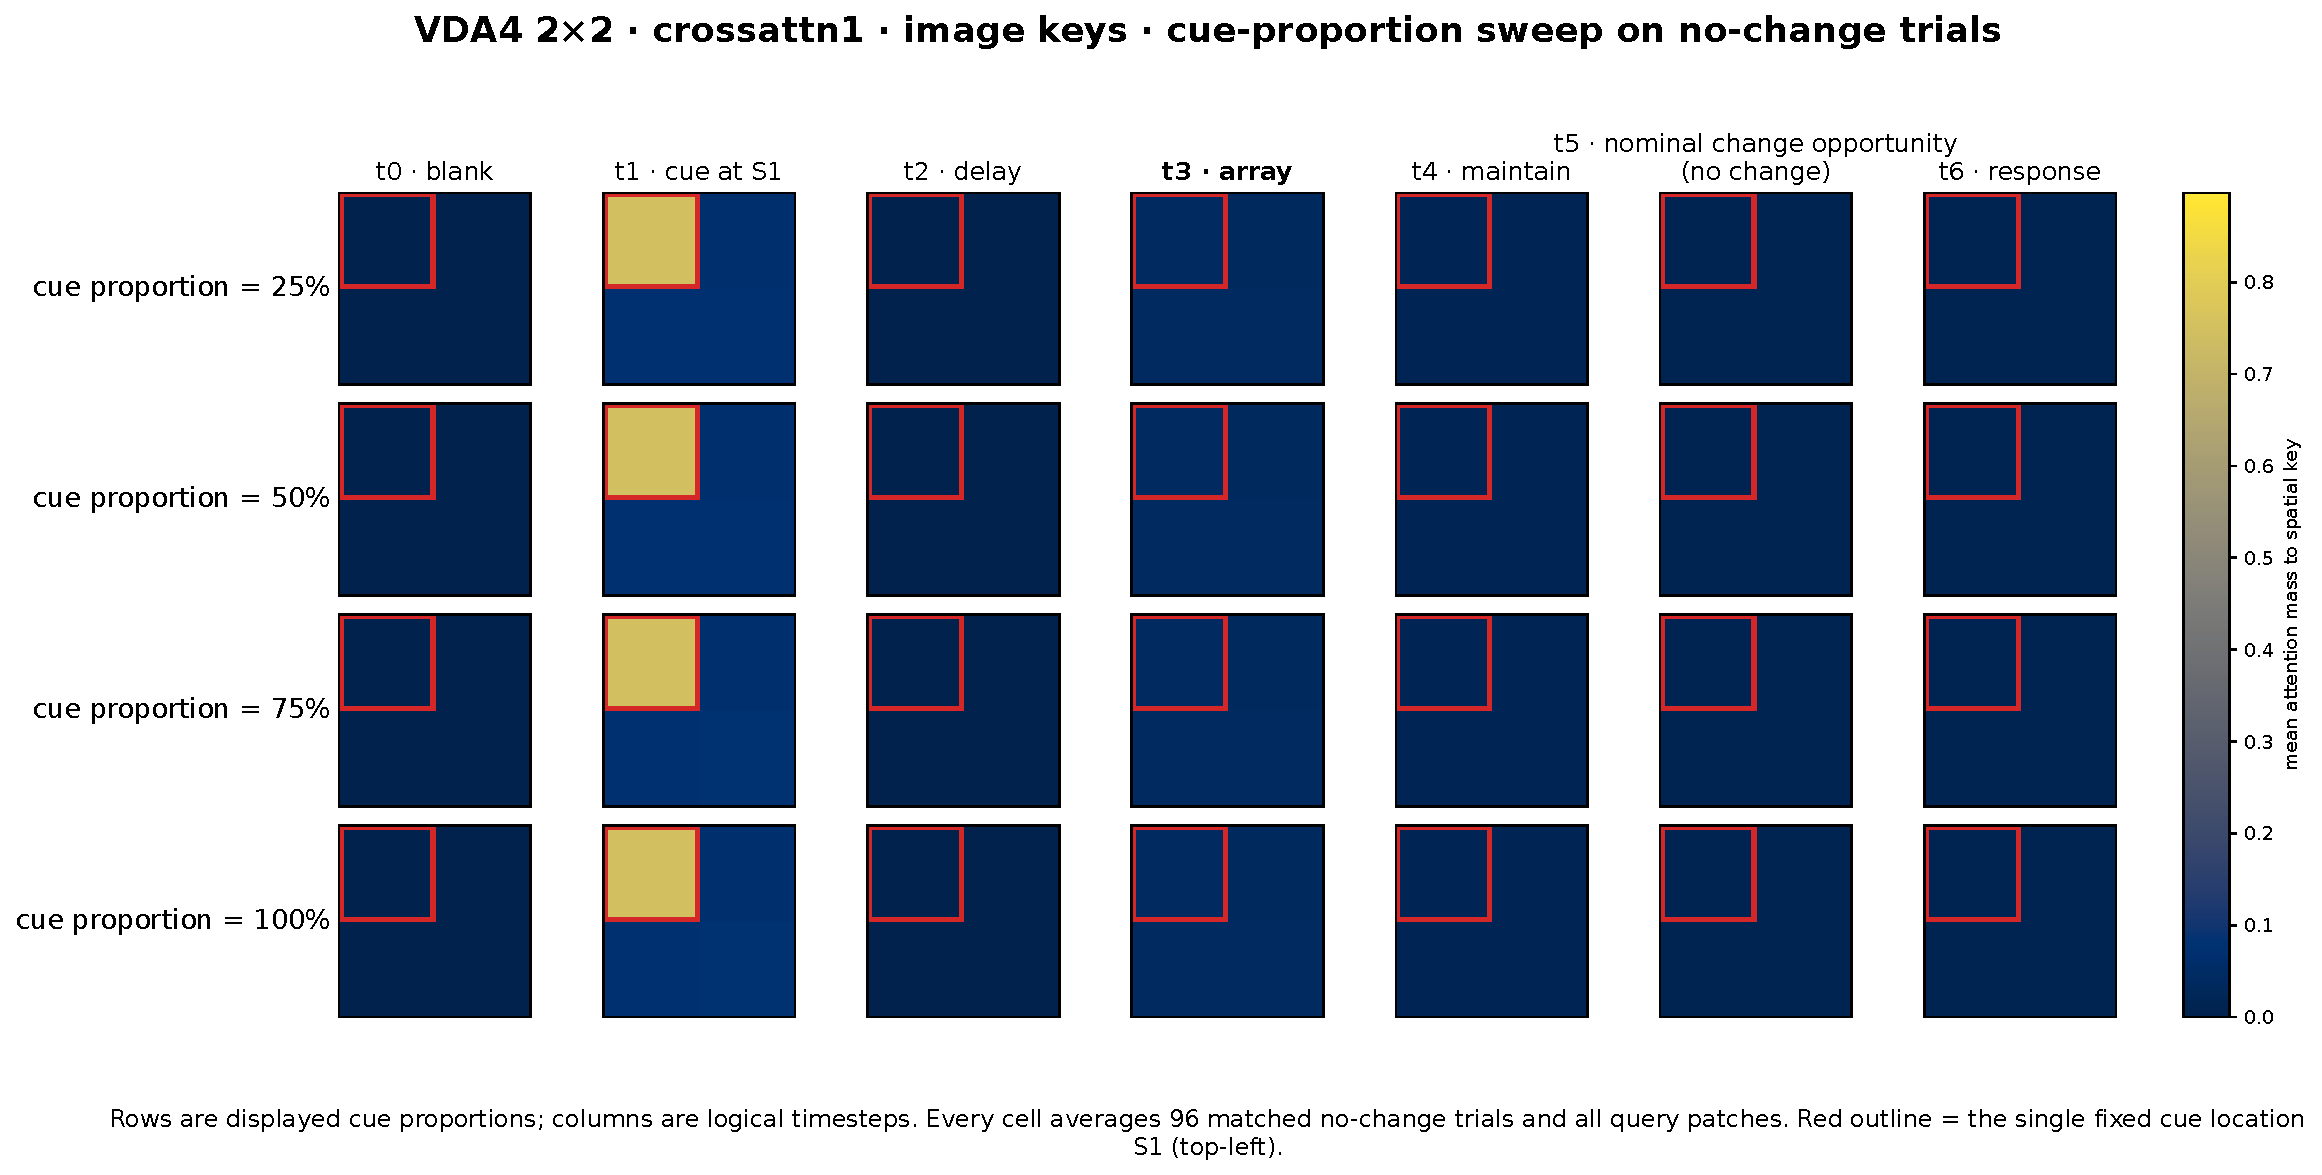
\includegraphics[width=0.32\textwidth]{first_wave_attention_vda4_crossattn1_image_keys.pdf}\hfill
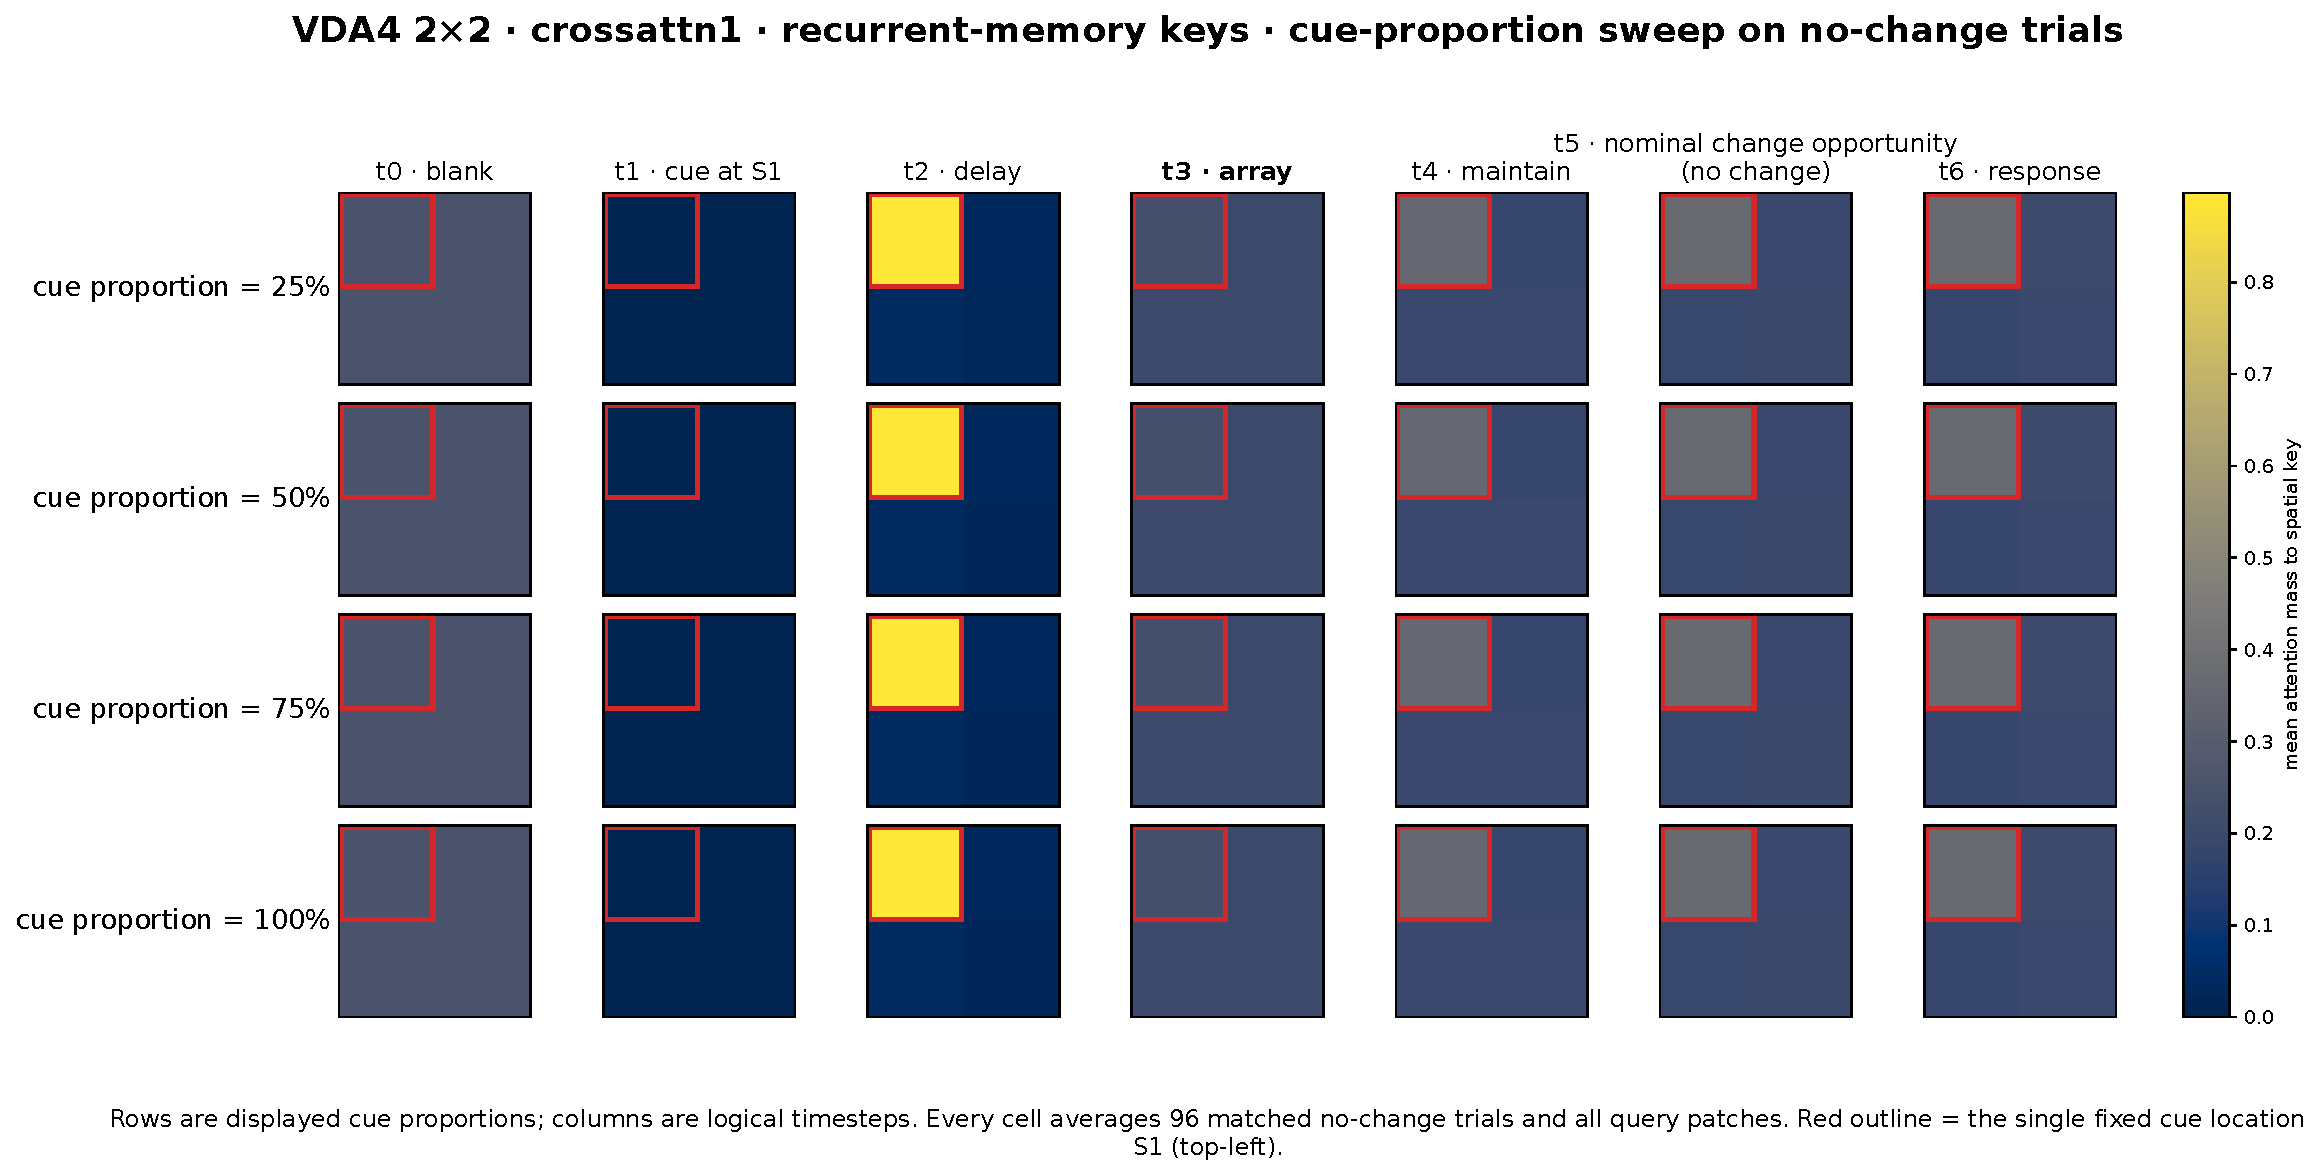
\includegraphics[width=0.32\textwidth]{first_wave_attention_vda4_crossattn1_recurrent_memory_keys.pdf}\\[4pt]
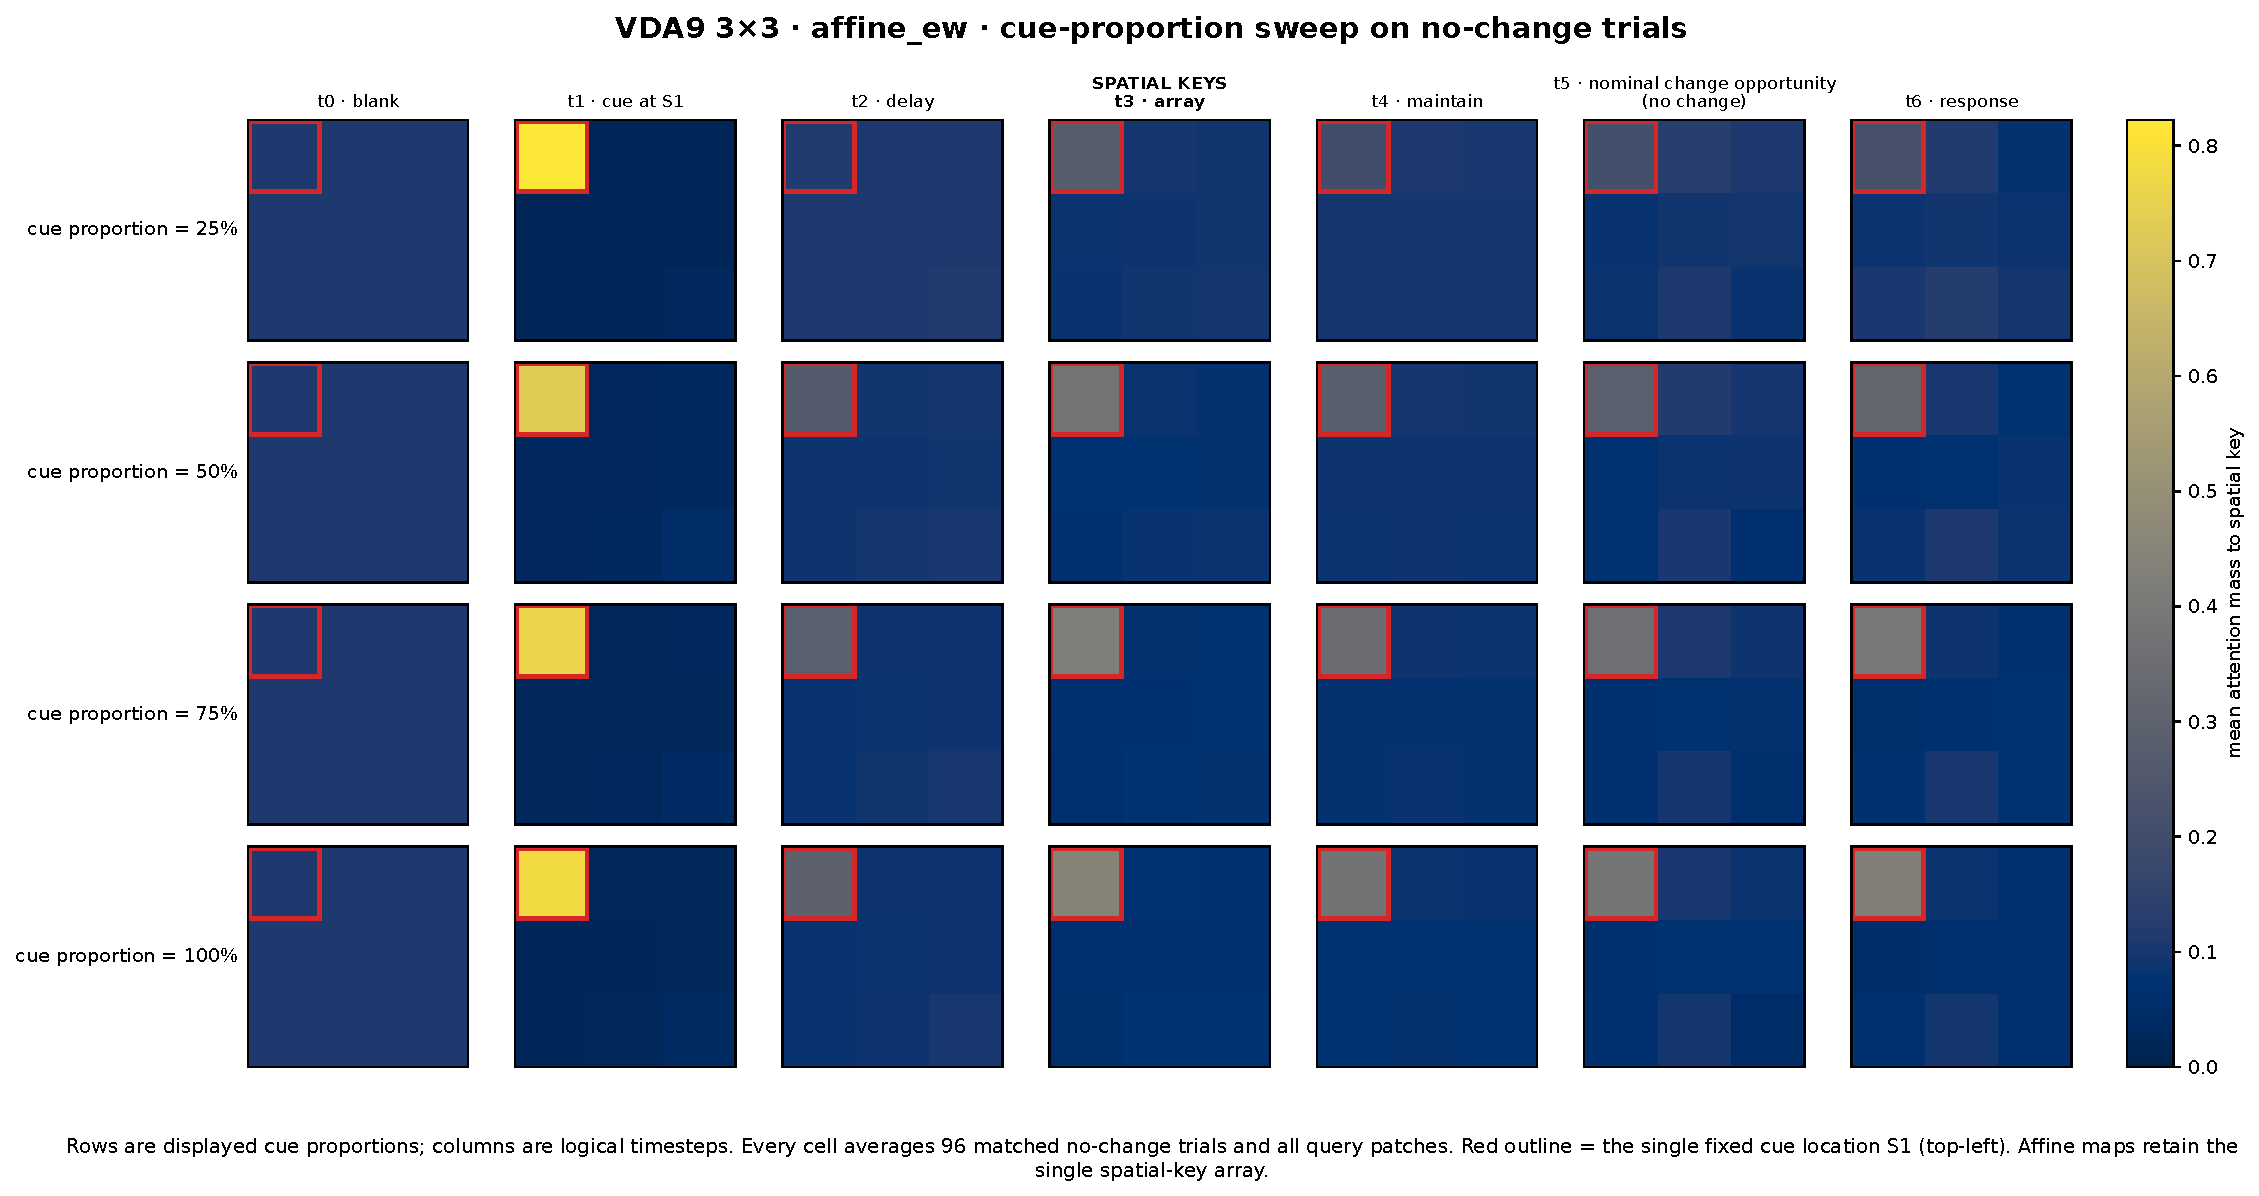
\includegraphics[width=0.32\textwidth]{first_wave_attention_vda9_affine_ew.pdf}\hfill
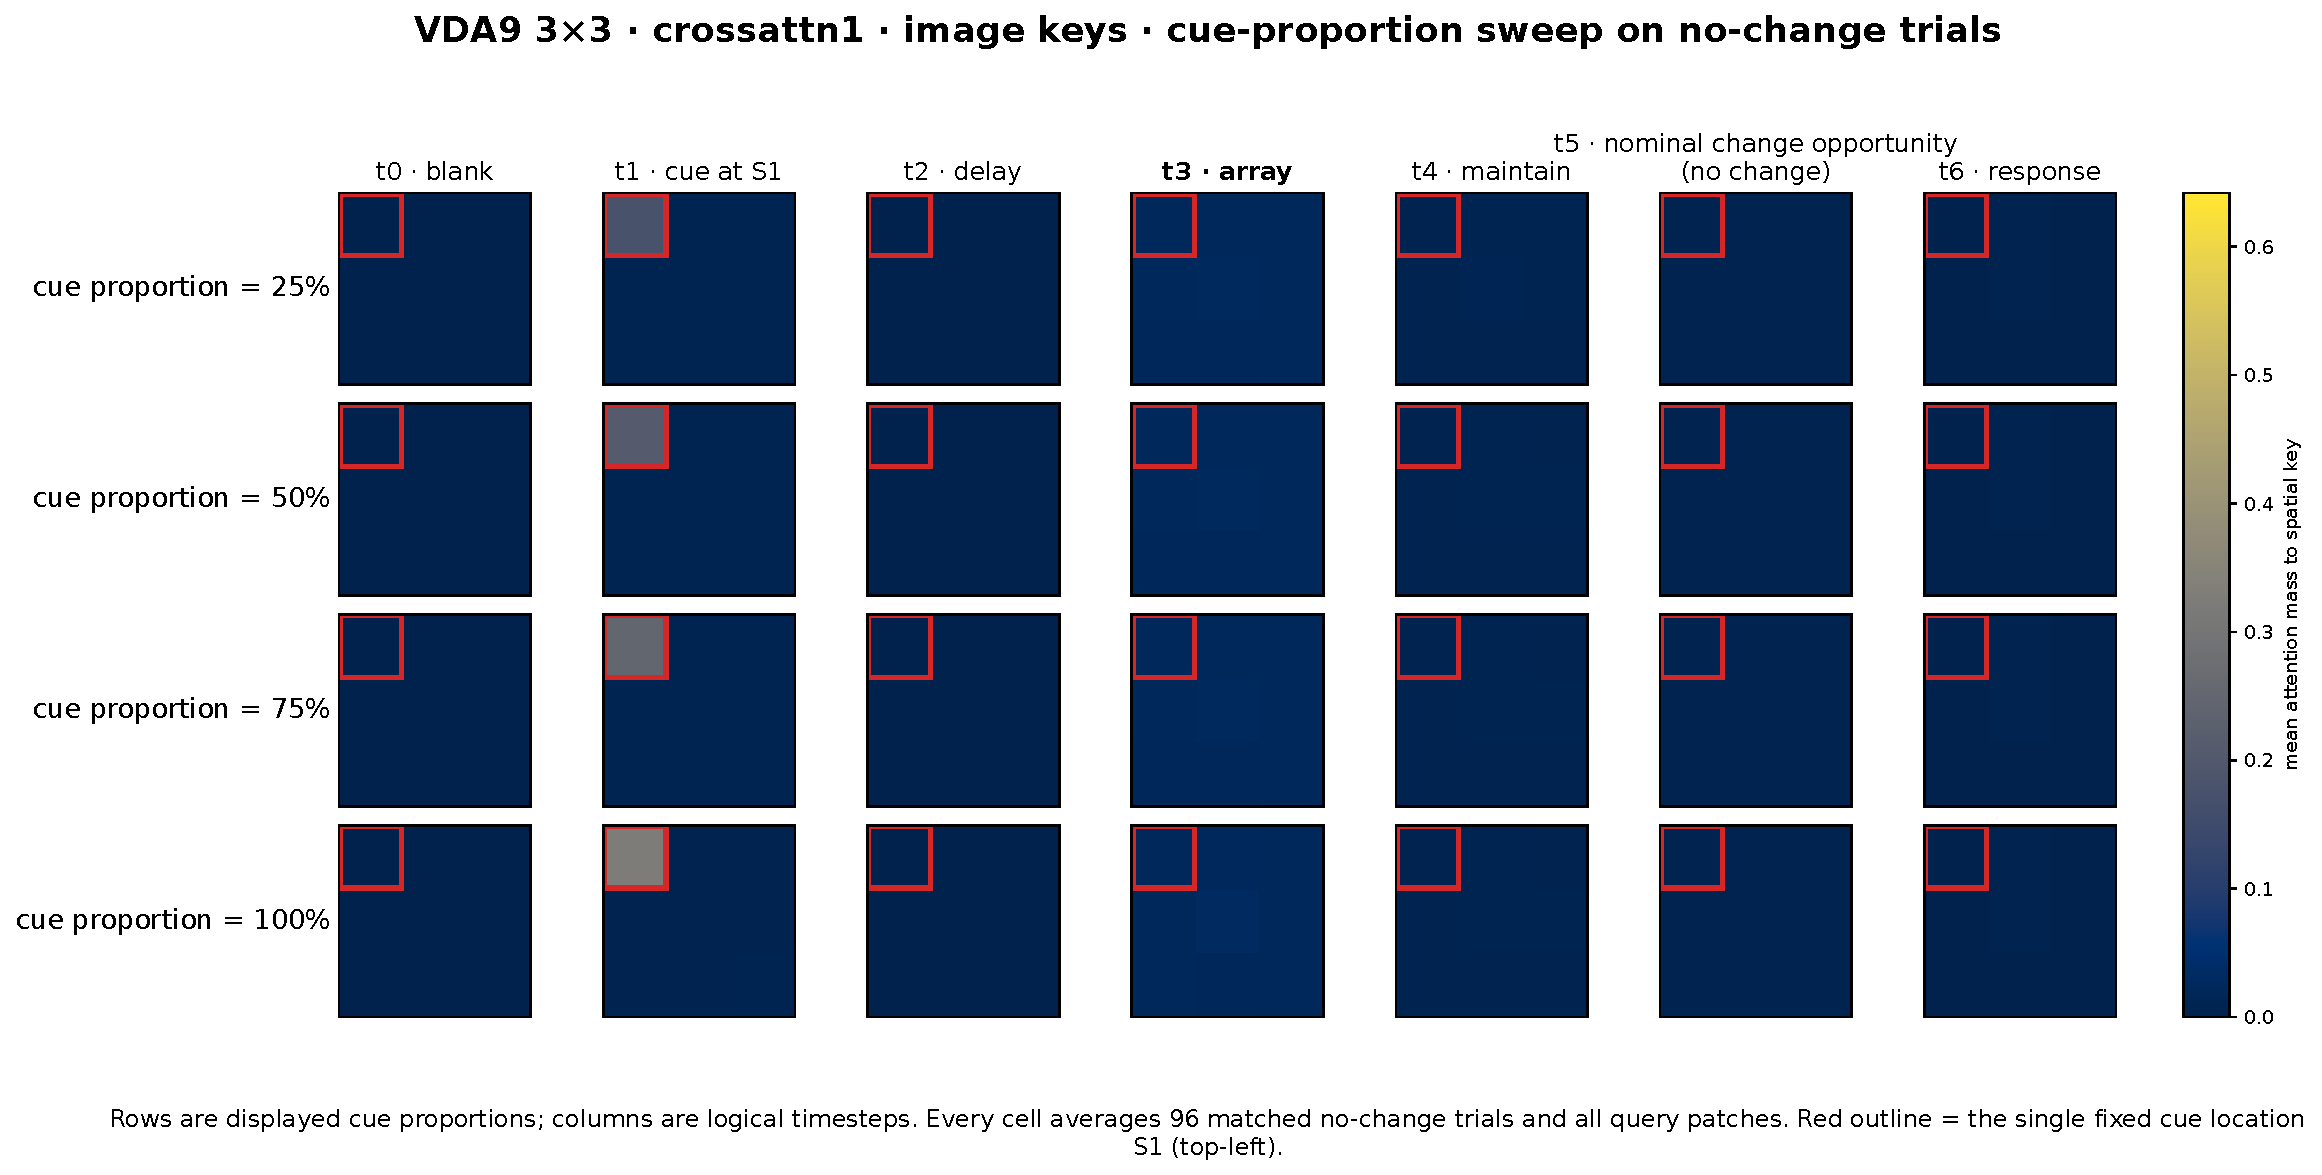
\includegraphics[width=0.32\textwidth]{first_wave_attention_vda9_crossattn1_image_keys.pdf}\hfill
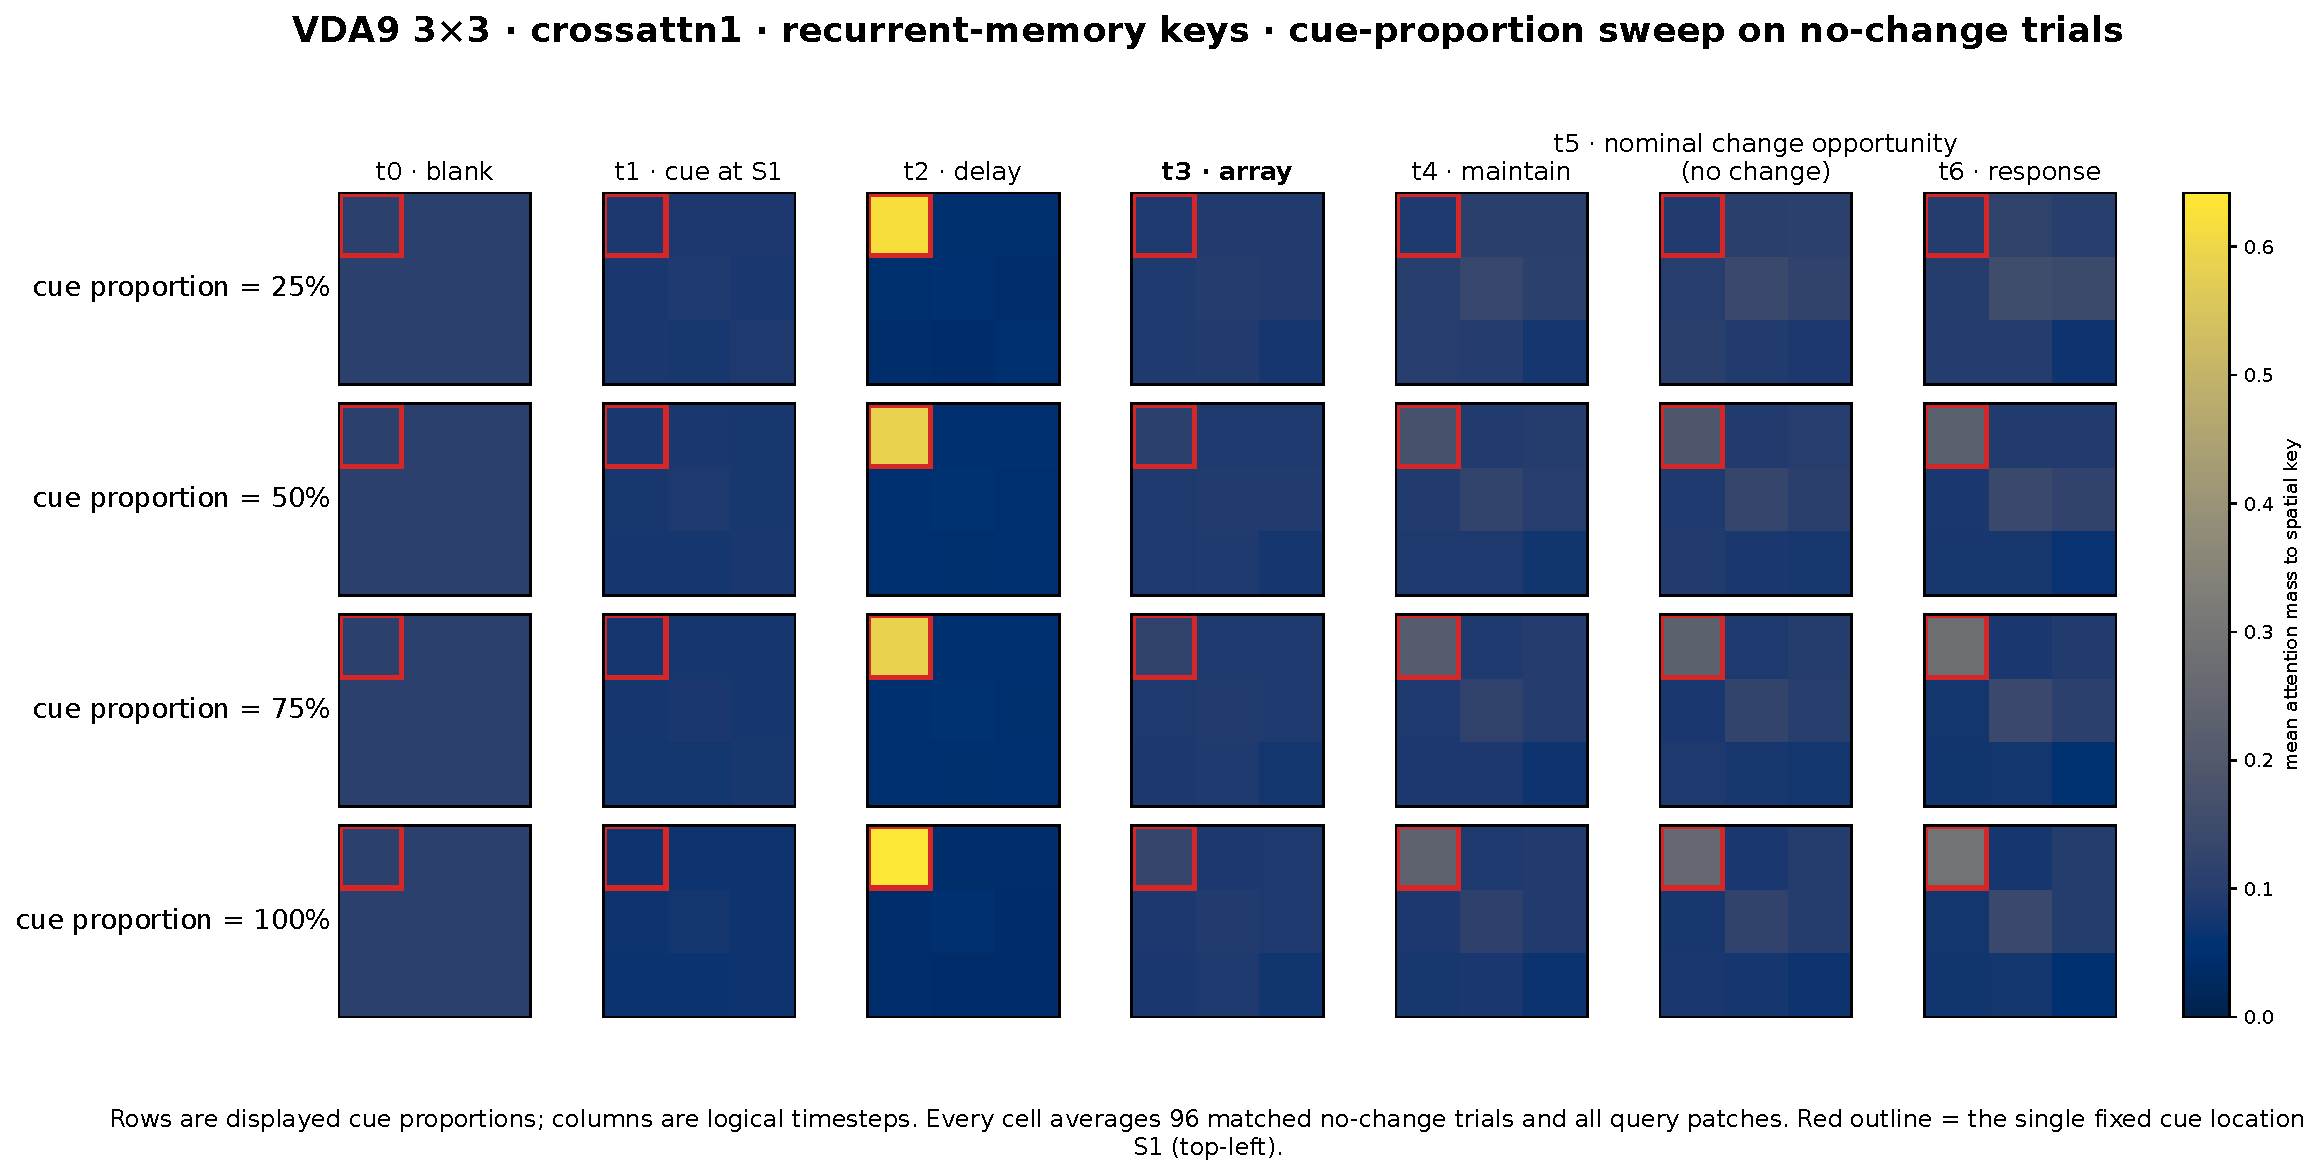
\includegraphics[width=0.32\textwidth]{first_wave_attention_vda9_crossattn1_recurrent_memory_keys.pdf}
\caption{\textbf{No-change-trial attention maps, VDA4 (top) and VDA9 (bottom).} Left to right: affine self-attention, cross-attention image keys, cross-attention memory keys. Rows are displayed cue proportion, columns are logical timesteps t0--t6; a red outline marks the fixed cue location. Because no physical change ever occurs, this evidence is completed by the paired VDA16 change-trial experiment in Section~\ref{sec:vda16-paired-attention}.}\label{fig:first-wave-attn}
\end{figure*}

\subsection{What a held-out probe reads from the recurrent state}\label{sec:width-decoding}
A regularized logistic probe, fit within each fold on train-only PCA-reduced state, reads change occurrence robustly everywhere (t6 balanced accuracy 0.76--0.90; Table~\ref{tab:decoder-scores}) and change location more variably (0.50--0.96, well above the relevant chance level). d256-minus-d128 differences vary in sign across pairs -- VDA4 affine gains 0.285 for change-location decoding, VDA4 cross-attention \emph{loses} 0.050 -- so \textbf{a wider checkpoint does not expose uniformly more decodable information} either, the representational counterpart to Section~\ref{sec:width-behavior}. \note{These scores establish information available to a linear readout at t6; they establish neither policy use nor persistent maintenance, and per Panichello and Buschman we do not claim a domain-general controller from a single task's decoder \cite{panichello2021}.}

\begin{table}[t]
\centering\small
\begin{tabularx}{\linewidth}{@{}l l Y Y@{}}
\toprule
Task & Routing & Change occ.\ (d128/d256) & Change loc.\ (d128/d256)\\
\midrule
VDA1 & affine & .893/.902 & undefined\\
VDA1 & cross-attn & .897/.888 & undefined\\
VDA4 & affine & .830/.879 & .616/.900\\
VDA4 & cross-attn & .818/.833 & .842/.792\\
VDA9 & affine & .761/.792 & .654/.499\\
\bottomrule
\end{tabularx}
\caption{Final-timestep (t6) held-out decoder balanced accuracy. Location targets undefined for singleton VDA1.}\label{tab:decoder-scores}
\end{table}

\subsection{VDA16 attention maps and readout}\label{sec:vda16-attention-dynamics}
The same no-change protocol at set size 16 shows the strongest cue-localized mass in cross-attention's recurrent-memory source at t2 -- after the cue, before the array -- while image-key cue mass at t1 grows with displayed cue proportion; affine's single self-attention array shows a strong S1 concentration at cue onset that persists, more weakly, through delay, array, and response (Figure~\ref{fig:vda16-attn}). A sustained cue-directed elevation during an empty delay is the pattern Awh and Jonides's overlapping-mechanisms account predicts if spatial attention supports rehearsal \cite{awh2001} -- \note{routing mass during delay is suggestive, not proof of rehearsal in the behavioral sense, which needs a delay-period disruption test we have not run.}

\begin{figure*}[t]
\centering

\includegraphics[width=0.32\textwidth]{first_wave_attention_vda16_crossattn1_image_keys.pdf}\hfill

\includegraphics[width=0.32\textwidth]{first_wave_attention_vda16_crossattn1_recurrent_memory_keys.pdf}\hfill
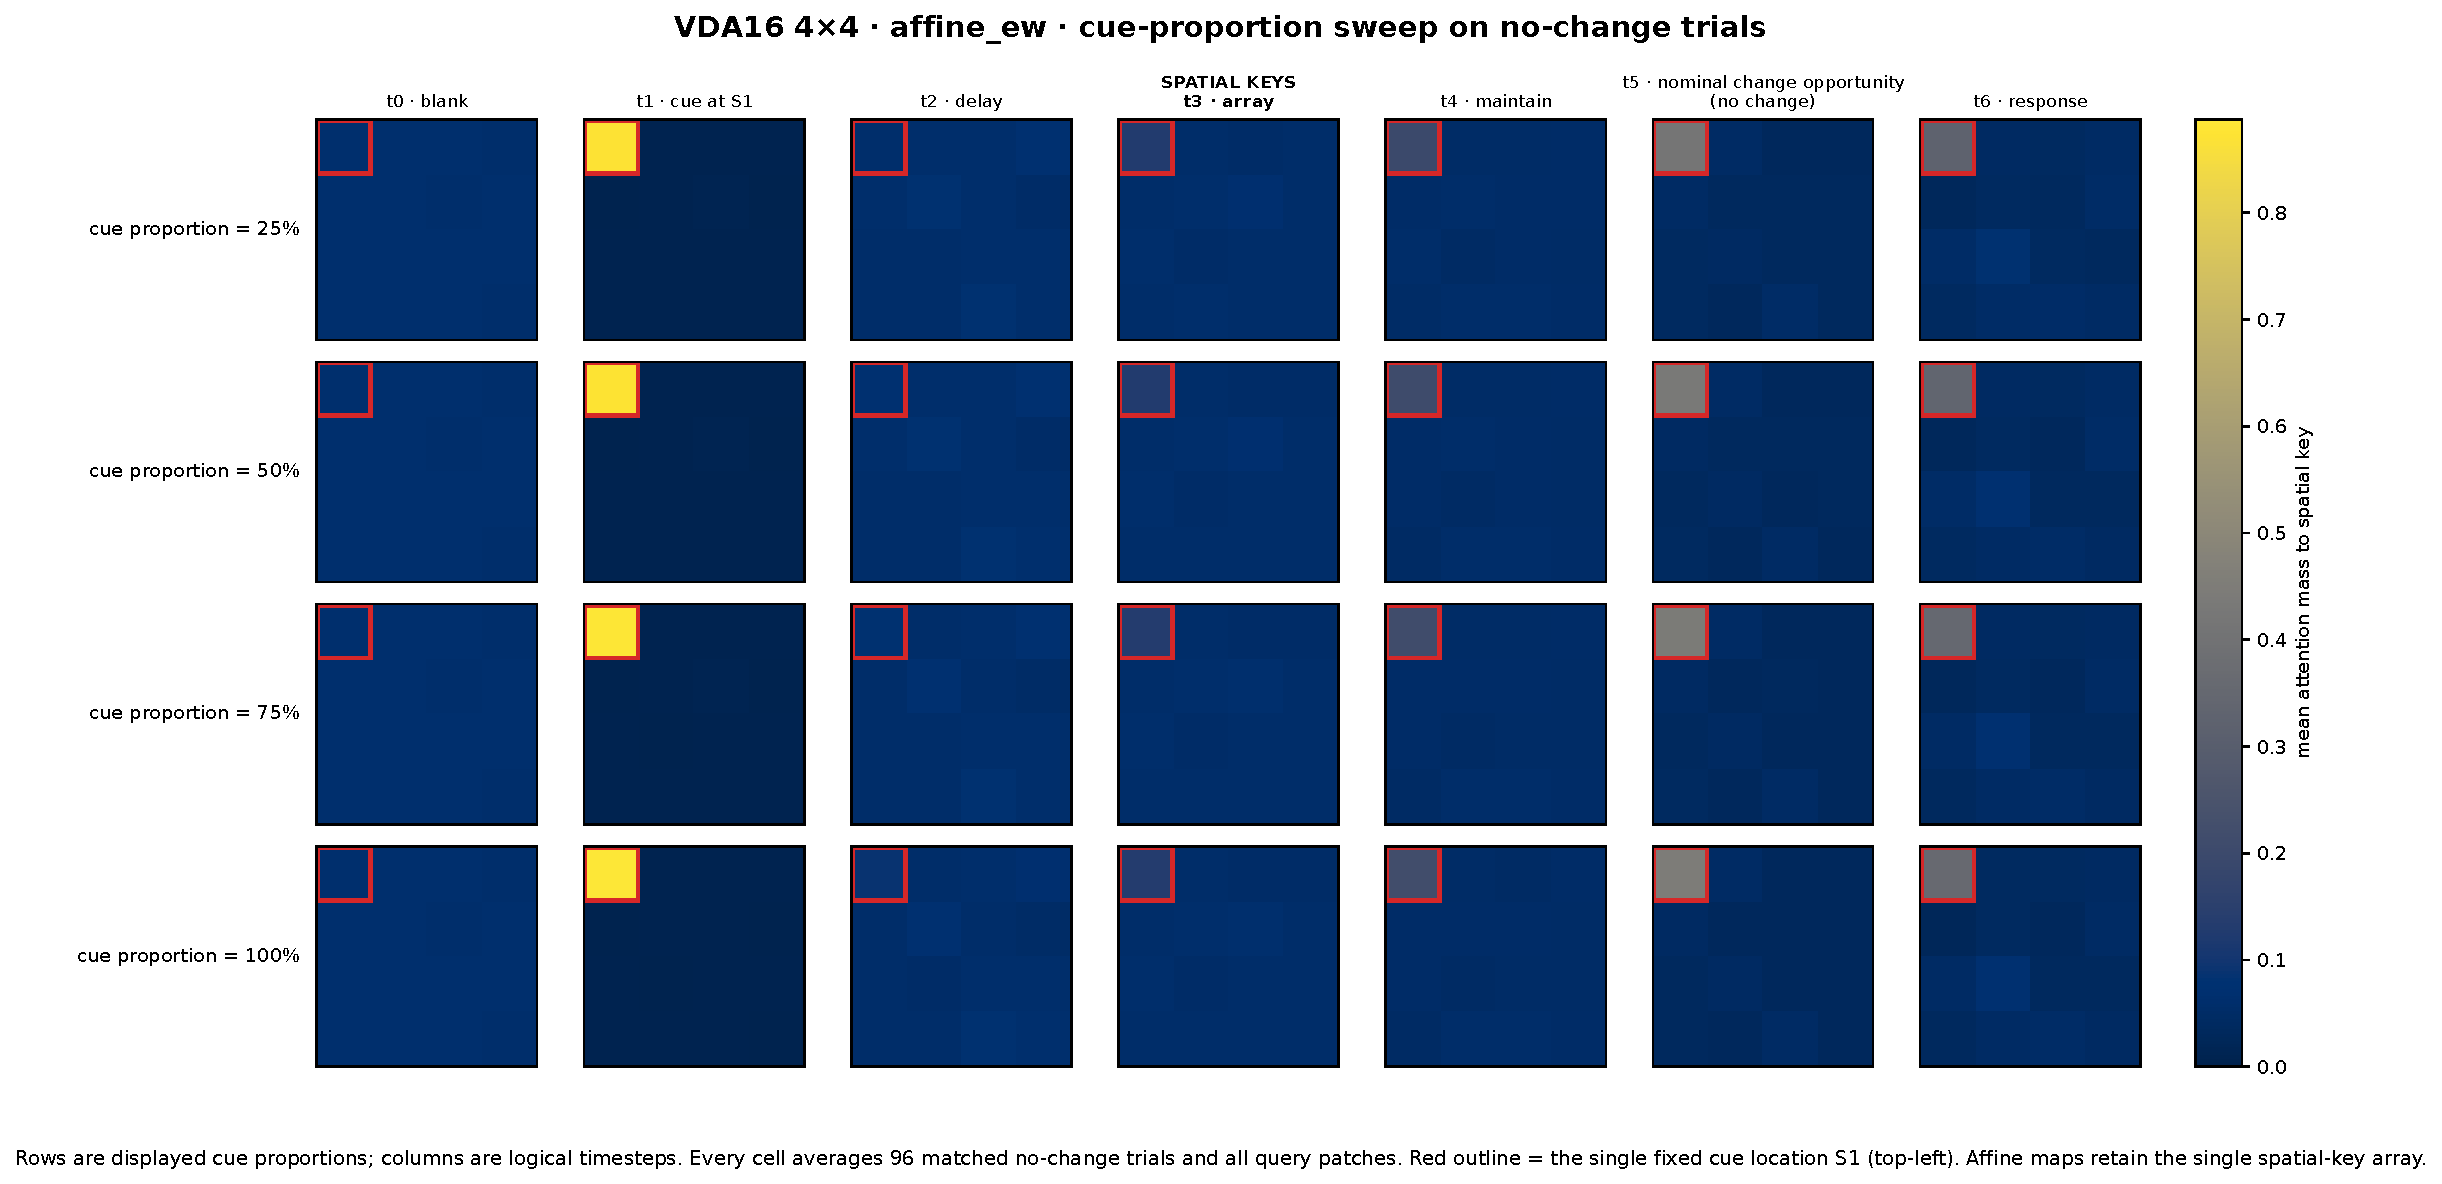
\includegraphics[width=0.32\textwidth]{first_wave_attention_vda16_affine_ew.pdf}
\caption{\textbf{VDA16 no-change-trial attention maps.} Left/center: cross-attention image and memory keys. Right: affine's single self-attention array. Same layout as Figure~\ref{fig:first-wave-attn}.}\label{fig:vda16-attn}
\end{figure*}

\subsection{Attention tracks the change location, weakly so when uncued}\label{sec:vda16-paired-attention}
The clearest all-timestep, valid-vs-invalid time course comes from the paired VDA16 rerun of Section~\ref{sec:vda16-behavior}, which -- unlike the maps above -- includes a real physical change. Achieved spatial attention (image-key $+$ memory-key mass, averaged over query tokens; uniform allocation $=0.0625$) at the $30^\circ$ focal change is \textbf{0.148 at cued S1 vs.\ 0.058 at uncued S16 four frames before the change} (t4; paired difference $+0.089$, 95\% CI 0.079--0.100) -- attributable to the cue alone. On the change frame itself (t5), means are 0.102 vs.\ 0.062 ($+0.041$, CI 0.030--0.051): the physical change pulls some weight toward S16 even though it was never cued, but far less than the cue alone had already pulled toward S1 (Figure~\ref{fig:vda16-paired}). This is the attentional mirror of Section~\ref{sec:vda16-behavior}'s behavioral gap, and it is exactly the deficit Section~\ref{sec:intervention} tests causally.

\begin{figure*}[t]
\centering

\includegraphics[width=0.49\textwidth]{vda16_cued_vs_opposite_summary.pdf}\hfill

\includegraphics[width=0.49\textwidth]{vda16_cued_vs_opposite_spatial_maps.pdf}
\caption{\textbf{The model looks less at a change it was not cued to expect.} Left: (A) response probability, (B) response timing, (C) achieved attention at the changed location on t5, (D) full seven-frame trajectory at $30^\circ$. Right: spatial attention maps at t4/t5, cued-S1 (top) vs.\ forced-S16 (bottom) changes; red = cue, green dashed = true change location. 300 trials/condition, common random numbers.}\label{fig:vda16-paired}
\end{figure*}

\subsection{An architectural finding: memory decay trades off against attention stability}\label{sec:architecture-thread}
A separate manipulation fixes VDA4 and varies only the recurrent cell's carried-state decay rate $\lambda$ between two otherwise-matched frozen checkpoints: standard ($\lambda=1.00$, no forgetting) vs.\ high-decay ($\lambda=0.80$). Measuring attention activity as frame-to-frame total variation over the full softmax map (not total mass, which is fixed to 1), the high-decay checkpoint is reliably more volatile: $+0.108$ total variation (95\% CI $+0.104$ to $+0.112$), with a cross-attention decay series showing the same direction across intermediate $\lambda$. \textbf{Faster forgetting produces more erratic routing, not less} -- a memory that retains information longer also holds its spatial routing steadier. This connects directly to the persistent-activity literature's proposed substrate for stable working-memory maintenance across a delay \cite{luck1997,awh2001}: within this architecture, sustained attention and memory persistence are two readouts of one decay parameter, not independent design choices. \note{Two checkpoints, one seed per arm, VDA4 only -- evidence that decay rate and stability covary in this architecture, not a claim about optimal decay or biological timescales.}

\FloatBarrier
\section{Attention Manipulation}\label{sec:intervention}
Everything so far is correlational: routing tracks the cue, and behavior tracks the cue, but neither fact shows that routing \emph{causes} behavior. Two classic experiments made exactly that causal move in biology. Moore and Armstrong's frontal-eye-field microstimulation retinotopically improved discrimination at the stimulated location \cite{moore2003}. Cavanaugh and Wurtz's subcortical stimulation counteracted change blindness, restoring detection at a location the animal would otherwise miss \cite{cavanaugh2004}. Both depend on the intervention being spatially matched to a named location and compared against non-matching locations -- not merely on ``stimulation changed behavior.'' This section runs the model-level analogue of both experiments on the same architecture.

\subsection{An existing lever: biasing the cued location changes sensitivity}\label{sec:existing-intervention}
Every attention module in this architecture accepts an explicit additive bias on named spatial keys before the softmax, independent of how the trial itself was generated: $s'_{tqk}=s_{tqk}+b\,\mathbf{1}[t\geq5]\,\mathbf{1}[k\in\mathcal{K}_{\mathrm{cue}}]$, $b\in\{-6,-3,0,3,6\}$, applied at the \emph{cued} location from t5 onward. This already establishes the bias is response-causal, with signal detection theory computed as $d'=\Phi^{-1}(H)-\Phi^{-1}(F)$, $c=-\tfrac12[\Phi^{-1}(H)+\Phi^{-1}(F)]$: at $b=-6$, VDA4 affine's within-checkpoint $d'$ drop differs from its d256 pair by $W=0.893$, while cross-attention's differs by $W=-0.192$ -- a sign reversal across checkpoints (Figure~\ref{fig:matched-width}C--D), so the effect of biasing the cued location is itself architecture-dependent.

At set size 16, cross-attention's sensitivity to this bias is broadly monotonic in both conditions; affine's is not (Figure~\ref{fig:vda16-clamp}). Affine's valid-trial $d'$ rises with bias, peaks at $2.87$ ($b=+3$), and eases to $2.76$; its invalid-trial $d'$ instead falls \emph{monotonically}, from $1.73$ at $b=-6$ to $0.58$ at $b=+6$ -- even though the bias always targets the cued location, never the true (uncued) change location. Achieved attention mass confirms why: boosting the cued key pulls routing mass toward it on invalid trials too (t6 mass $0.001\to0.134\to0.796$ across the sweep), so pushing more attention onto a location that is wrong on an invalid trial actively degrades detection elsewhere. That competitive logic -- biasing the wrong location can hurt, not help -- is the question the rest of this section tests directly, with the bias placed at the correct location instead.

\begin{figure*}[t]
\centering

\includegraphics[width=0.49\textwidth]{vda16_clamp_achieved_attention.pdf}\hfill
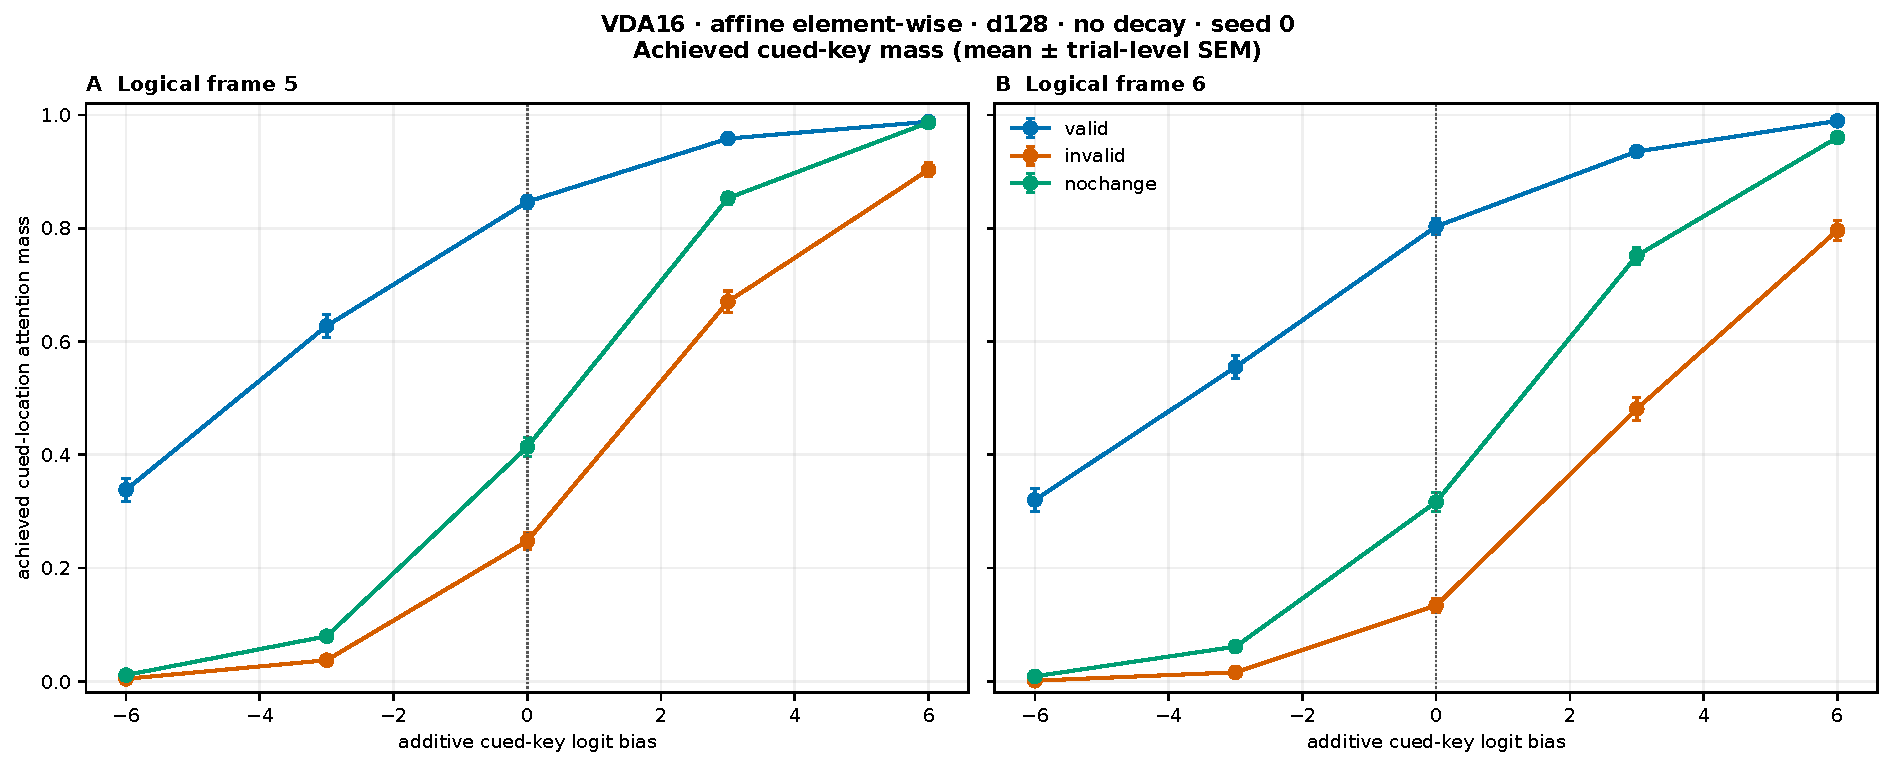
\includegraphics[width=0.49\textwidth]{vda16_affine_clamp_achieved_attention.pdf}
\caption{\textbf{Achieved cued-location attention mass under the additive bias sweep, cross-attention (left) and affine (right).} Both routing families' achieved attention rises smoothly with nominal bias; only affine's \emph{invalid-trial} sensitivity falls monotonically as that mass grows, because the boosted location is the wrong one on invalid trials.}\label{fig:vda16-clamp}
\end{figure*}

\subsection{The rescue test: biasing the true change location}\label{sec:pending-intervention}
The lever above always targets the location the cue points to, whether or not that location changes. Here we instead target the \emph{true change location on an invalid-cue trial} -- the condition that directly tests the Moore--Armstrong/Cavanaugh--Wurtz logic on this model. Section~\ref{sec:vda16-paired-attention} showed achieved attention at an uncued change location is roughly a third of its cued value even after the change occurs, tracking a behavioral gap from 0.983 to 0.490 qualifying response rate at the same focal magnitude. If that routing deficit is what \emph{causes} the behavioral deficit, restoring it by force should recover behavior, and removing it further should make an already-poor trial worse.

On trials with the change forced away from the cue (300 trials/condition, common random numbers, $30^\circ$ focal magnitude, cross-attention checkpoint), we sweep the identical graded bias independently at three locations: the true change location (the test itself), the cued-but-wrong location (negative control), and a fourth, task-irrelevant location (spatial-specificity control). All three reuse the primitives above with no new model code.

\textbf{Targeting the true change location produces the predicted double dissociation} (Figure~\ref{fig:change-loc}). Relative to the unbiased invalid-trial baseline ($51\%$ qualifying response rate, $d'=1.91$): full suppression collapses detection to \textbf{7\%} ($d'=0.38$); full boost recovers it to \textbf{95\%} ($d'=3.33$), closing \textbf{92\%} of the gap to the independently measured valid-trial ceiling of 98\%. Achieved attention at the true change location tracks this exactly -- suppression drives it to zero from the moment the bias switches on; boost drives it to 99\% by the response frame, against 33\% at baseline. Response timing among trials that do respond barely moves (5.5--6.0 frames throughout): \textbf{the intervention changes whether the model detects the change, not how quickly it responds once it does.}

Neither control location reproduces the rescue. Suppressing the cued-but-wrong location barely moves response rate ($51\%\to54\%$); boosting it instead \emph{lowers} response rate to $42\%$ and nearly quadruples the false-alarm rate ($3\%\to25\%$) -- a less stable, more trigger-happy policy, not improved detection. Suppressing the neutral location is similarly inert ($51\%\to53\%$); boosting it drops response rate to $9\%$, comparably severe to suppressing the true change location itself. Achieved attention at the true change location falls to 7\% (cued-boost) and 3\% (neutral-boost) of baseline, so the impairment reads as competitive -- forcing routing weight elsewhere pulls it away from where it is needed, rather than adding a generic, location-independent gain. \textbf{The rescue is spatially specific to the true change location. It is not an artifact of biasing attention anywhere.}

\begin{figure*}[t]
\centering
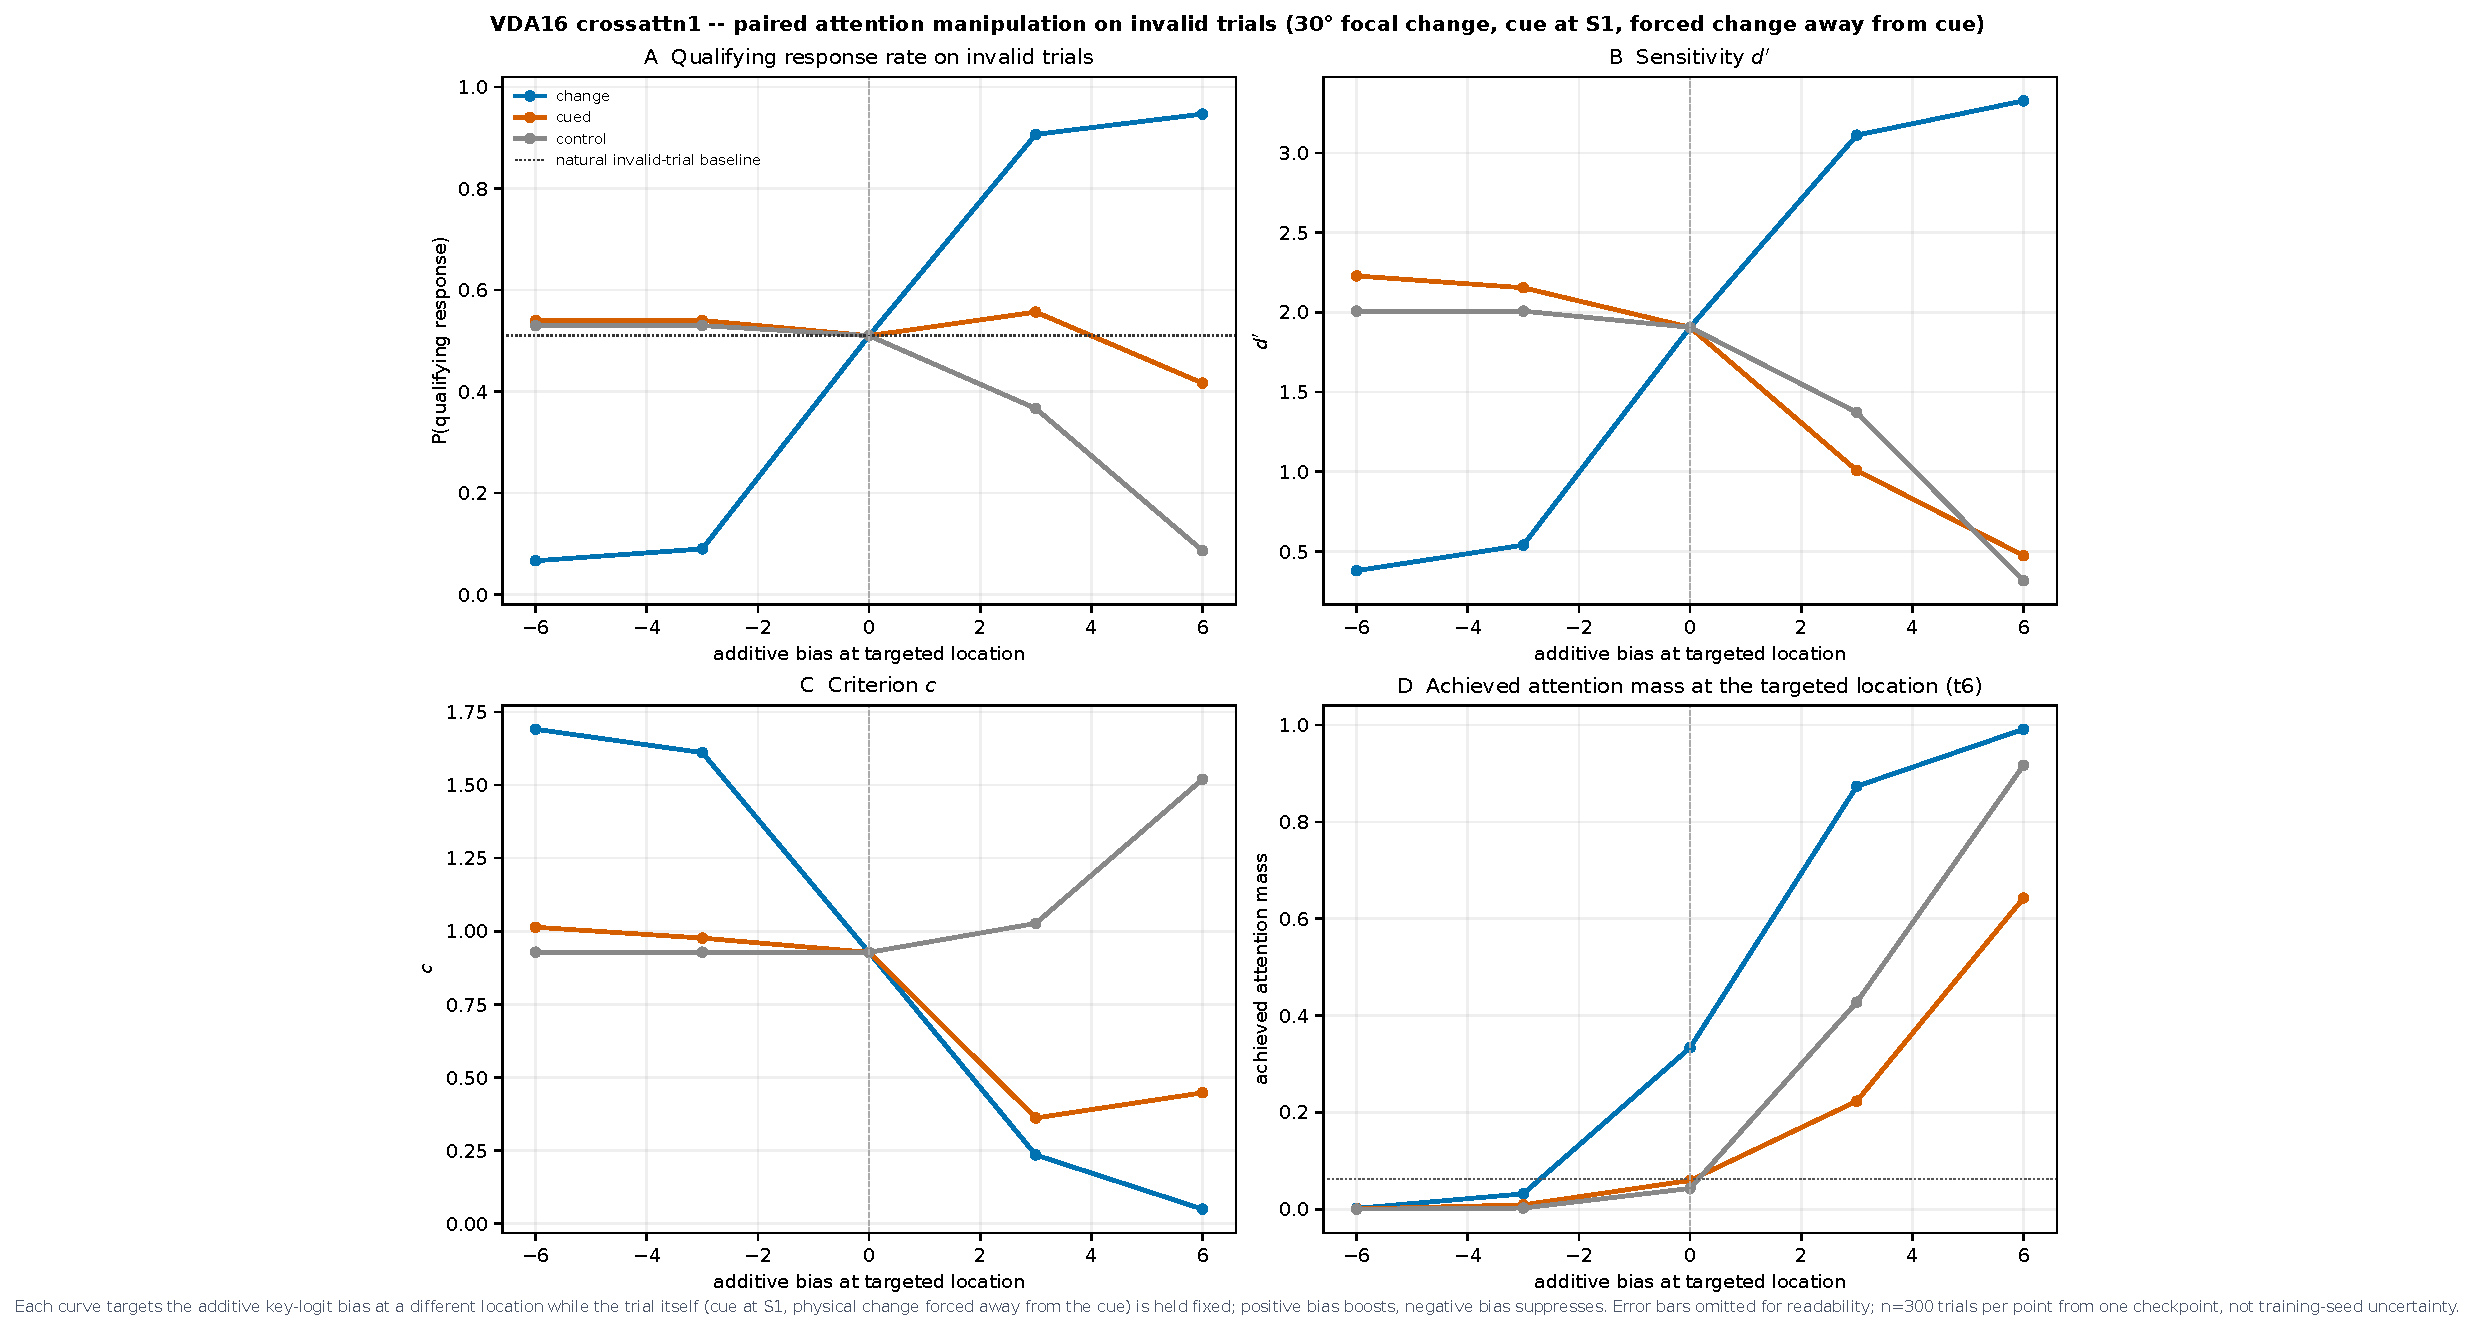
\includegraphics[width=0.85\textwidth]{vda16_change_location_intervention_summary.pdf}
\caption{\textbf{The central result of this paper: a spatially specific causal double dissociation.} On invalid-cue trials, the same graded bias is targeted independently at the true change location, the cued-but-wrong location, or a neutral location. (A) Qualifying response rate -- only the true-change-location curve rescues detection; the dotted line marks the unbiased baseline. (B) Sensitivity $d'$. (C) Criterion $c$. (D) Achieved attention at the targeted location. Cross-attention, VDA16, one competence-gated checkpoint, 300 trials/condition.}\label{fig:change-loc}
\end{figure*}

\begin{figure}[t]
\centering
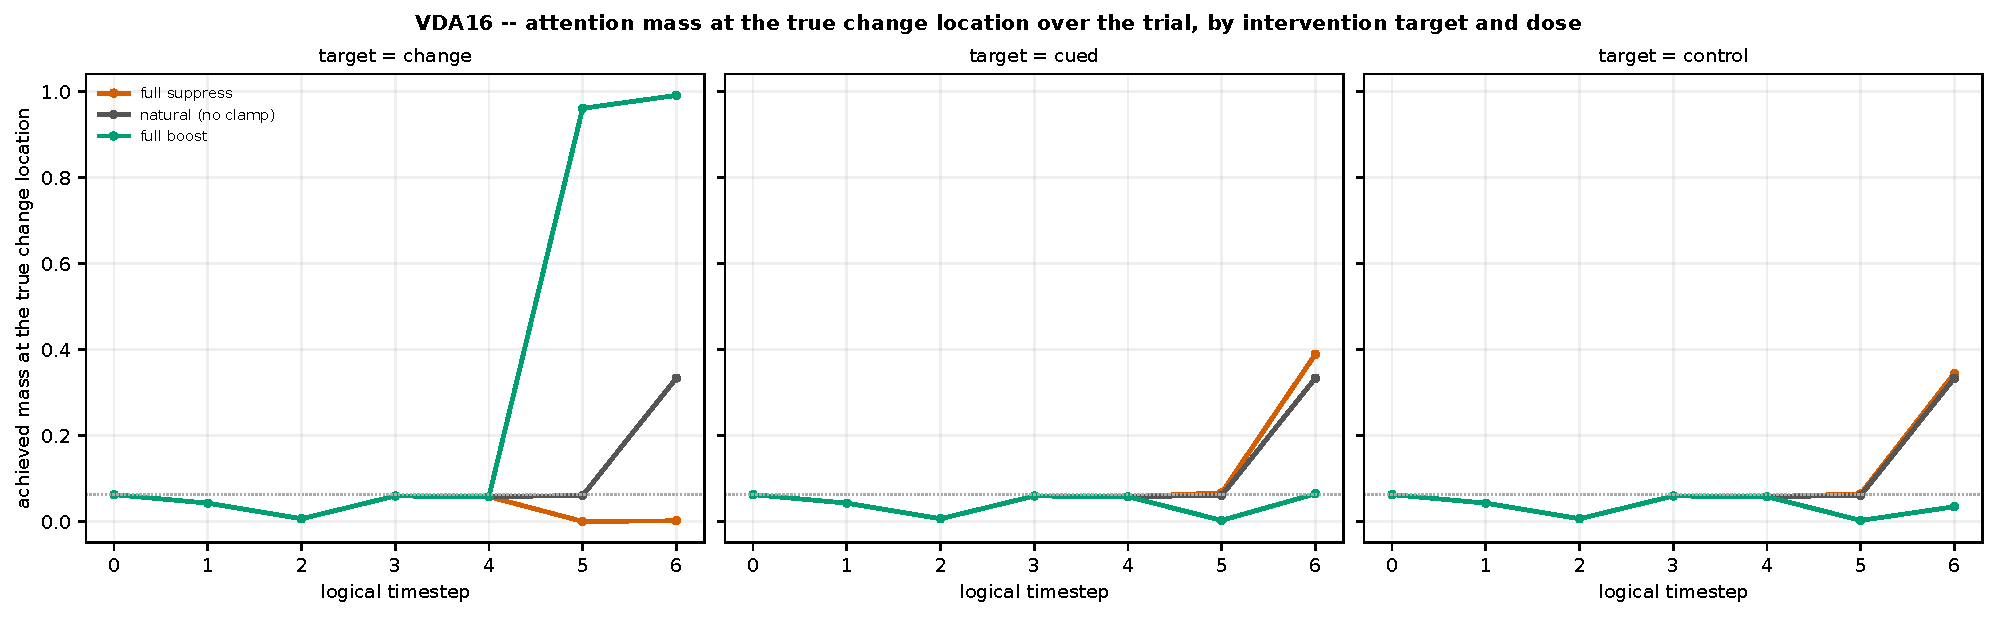
\includegraphics[width=\linewidth]{vda16_change_location_attention_trajectory.pdf}
\caption{\textbf{Achieved attention at the true change location across the full trial, by intervention target.} Only directly targeting the true change location moves its own achieved mass upward; boosting either control location competitively \emph{reduces} it below baseline instead.}\label{fig:change-loc-trajectory}
\end{figure}

\note{This is a single-checkpoint, finite-trial result on one competence-gated VDA16 seed. It establishes that this checkpoint's routing at the true change location is both necessary and sufficient for its invalid-trial detection, and that the effect is spatially specific rather than a generic gain change -- a model-level counterpart to the Moore--Armstrong/Cavanaugh--Wurtz logic, not evidence of biological equivalence. It does not establish training-seed generality or whether the same dissociation holds at smaller set sizes: the identical battery is specified for VDA4 and VDA9 to test whether the rescue effect itself scales with set size, and is blocked in this environment by missing checkpoint files (not by design) rather than run.}

\FloatBarrier
\section{Discussion: What Did We Learn About Attention?}\label{sec:discussion}
\textbf{Attention-like routing in this model is not epiphenomenal.} That is the central claim this paper defends. It would have been entirely possible for the model's internal routing to correlate with the cue and with behavior without doing any causal work -- a decodable-but-unused signal is exactly what many probing studies in deep learning turn up. Instead, directly manipulating routing at a single, correctly identified location is both necessary (suppression abolishes an already-fragile detection) and sufficient (boosting it recovers 92\% of the valid-cue ceiling) for the model's behavior, and the effect vanishes -- or reverses -- when the identical manipulation targets a plausible but incorrect location. That double dissociation, not the raw existence of a cueing effect, is what licenses calling this routing a model-level counterpart of spatial attention rather than a correlate of it.

\textbf{Attention here is inseparable from working memory.} The routing that gets causally rescued in Section~\ref{sec:pending-intervention} is carried by the same recurrent state whose decay rate we manipulate in Section~\ref{sec:architecture-thread}. A memory that forgets faster produces routing that is more erratic frame to frame, not more flexible -- persistence and stability are two readouts of one parameter in this architecture, not independent design choices. That is a specific, falsifiable echo of the persistent-activity account of working-memory maintenance \cite{luck1997,awh2001}, obtained here as a directly manipulable property rather than an assumption.

\textbf{Neither set size nor width is a clean independent variable for the cueing benefit.} We built this paper's motivating claim -- larger set sizes produce a more dramatic cueing effect -- on the cross-attention checkpoints, where it holds cleanly and monotonically. The identical claim, tested on an affine checkpoint trained on the identical task, does not hold past set size 9. A parallel result already appears in Section~\ref{sec:width-behavior}: doubling recurrent width changes the cueing benefit's sign as often as its magnitude. Both results argue against treating ``set size'' or ``width'' as if either behaves like a scalar knob with a monotone effect on attention -- how the computation is implemented matters as much as how many items compete or how large the memory is, a caution that should generalize past this specific architecture.

\textbf{What remains open.} Three gaps matter most. First, set size is confounded with spatial discretization in the present design -- historical VDA4/VDA9 change grid geometry together with item count, while controlled VDA16 changes item count on a fixed, finer $4\times4$ grid. Placing VDA4 on that same $4\times4$ grid (\env{vda\_fixed4}, already registered but currently blocked by a missing checkpoint) would separate the two explanations; until then, the set-size story in Section~\ref{sec:psychometric-fits} is consistent with a true set-size effect but does not isolate one. Second, the rescue test has been run only on one VDA16 checkpoint; the identical VDA4/VDA9 battery would show whether the rescue effect itself scales with set size, the same way the underlying cueing benefit does. Third, criterion has been computed throughout but analyzed systematically only for the rescue test itself; Luo and Maunsell's warning that a more liberal policy can raise hit rate without improving discrimination is only partly answered by the flat false-alarm rate in Figure~\ref{fig:vda16-context}D, and a full sensitivity/criterion decomposition at every reported cueing effect is future work \cite{luo2018}.

\note{The admissible language throughout this paper is ``model-level counterpart,'' ``structurally analogous,'' or ``corresponds to.'' No result here identifies a routing tensor as FEF, SC, LPFC, or biological working memory, and none of it establishes population-level precision, training-seed replication, or human/primate capacity -- each would need independent training seeds, which this single-checkpoint design does not have.}

\FloatBarrier
\section{Methods and Reproducibility}\label{sec:methods}
Every quantitative or causal claim above traces to an explicit checkpoint and cached analysis artifact; provenance detail that would otherwise interrupt the narrative is summarized here rather than boxed beside every figure. Historical aggregates come from a preserved NPZ archive with no producer hash or per-point trial count and are never treated as more than a qualitative landscape. The first-wave, matched-width, and VDA16 batteries instead execute exact, hash-verified checkpoints after freezing source bytes, write immutable trial-level and reduced caches, and pass an independent read-only provenance audit; the matched-width battery's review returned \emph{approve with limits} (separate-checkpoint, finite-trial, and competence-gate limits remain explicitly active). VDA16's cross-attention checkpoint is competence-gated at curriculum angle $\theta=65^\circ$ (never advanced from initialization); its affine counterpart advanced further to $\theta=47^\circ$ after a statefully resumed training run recovered by saved checkpoint hashes; neither reached the declared $8^\circ$ floor. The change-location intervention (Section~\ref{sec:pending-intervention}) is produced by a new, independently written script (\texttt{change\_location\_intervention.py}) that reuses the existing, already-tested additive key-logit bias, forced-location trial generation, and signal-detection primitives rather than introducing new model code; its VDA4/VDA9 arms are recorded as explicitly blocked, with a manifest, rather than silently omitted. The logistic-fit re-analysis in Section~\ref{sec:psychometric-fits} performs no checkpoint or model access at all, only re-reading already-cached, already-verified response-probability arrays. The repository's regression suite (266 tests) covers cache and checkpoint identity, matched stimulus generation, decoder chance levels, and competence gating; every rendered page of this manuscript was visually inspected before compilation. Appendix~\ref{app:provenance} lists every artifact's path and provenance class; the coverage matrices in Appendices~\ref{app:coverage}--\ref{app:disposition} record, cell by cell, which of the 952 source-derived panel--environment estimands are complete, available, blocked, undefined, or inapplicable, so that absence of evidence is always a recorded, explained state rather than a silent gap.

\FloatBarrier
\section{Conclusion}
A recurrent vision transformer trained on cued visual change detection shows the behavioral and representational signatures of spatial cueing at every set size and routing family we tested, and -- in its cross-attention lineage specifically -- both signatures sharpen as set size grows from 4 to 16. But the paper's central contribution is causal, not correlational: biasing the model's own internal routing at the true, uncued location of a change collapses detection when suppressed and recovers 92\% of the valid-cue ceiling when boosted, while the identical manipulation at a plausible-but-wrong location does neither -- a spatially specific double dissociation that is the model-level analogue of the microstimulation and inactivation logic that first showed FEF and SC signals were not just correlated with primate attention, but caused it. A second, narrower finding is architectural rather than task-driven: recurrent memory decay rate and moment-to-moment routing stability covary in this model family, independent of task condition. Neither finding licenses a claim about human or primate capacity, and no routing tensor here is claimed to be a specific brain region; both are stated as model-level counterparts to a real, cited experimental tradition, with the evidentiary boundary of that correspondence given beside each claim rather than collected at the end.

\bibliographystyle{plain}
\begin{thebibliography}{9}
\small
\bibitem{mah2025} J.~Morgan, L.~Albanna, and J.~P.~Herman. Recurrent vision transformers model visual attention through feedback. \emph{arXiv:2502.10955v1}, 2025.
\bibitem{carrasco2011} M.~Carrasco. Visual attention: the past 25 years. \emph{Vision Research}, 2011.
\bibitem{herman2017} J.~P.~Herman and R.~J.~Krauzlis. Color-change detection activity in the primate superior colliculus. \emph{eNeuro}, 2017.
\bibitem{luo2018} T.~Z.~Luo and J.~H.~R.~Maunsell. Attentional changes in either criterion or sensitivity are associated with robust modulations in lateral prefrontal cortex. \emph{Neuron}, 2018.
\bibitem{moore2003} T.~Moore and K.~M.~Armstrong. Selective gating of visual signals by microstimulation of frontal cortex. \emph{Nature}, 2003.
\bibitem{cavanaugh2004} J.~Cavanaugh and R.~H.~Wurtz. Subcortical modulation of attention counters change blindness. \emph{Journal of Neuroscience}, 2004.
\bibitem{luck1997} S.~J.~Luck and E.~K.~Vogel. The capacity of visual working memory for features and conjunctions. \emph{Nature}, 1997.
\bibitem{awh2001} E.~Awh and J.~Jonides. Overlapping mechanisms of attention and spatial working memory. \emph{Trends in Cognitive Sciences}, 2001.
\bibitem{panichello2021} M.~F.~Panichello and T.~J.~Buschman. Shared mechanisms underlie the control of working memory and attention. \emph{Nature}, 2021.
\end{thebibliography}

\onecolumn
\appendix
\FloatBarrier
\section{Reference Material}
The results above are the paper; this appendix is the evidence trail behind them, kept in full because a claim this reliant on provenance (single checkpoints, hash-verified caches, explicit blocked/undefined states) should remain auditable. It is reference material, not required reading.

\subsection{Fourteen-environment task atlas}
\begin{center}
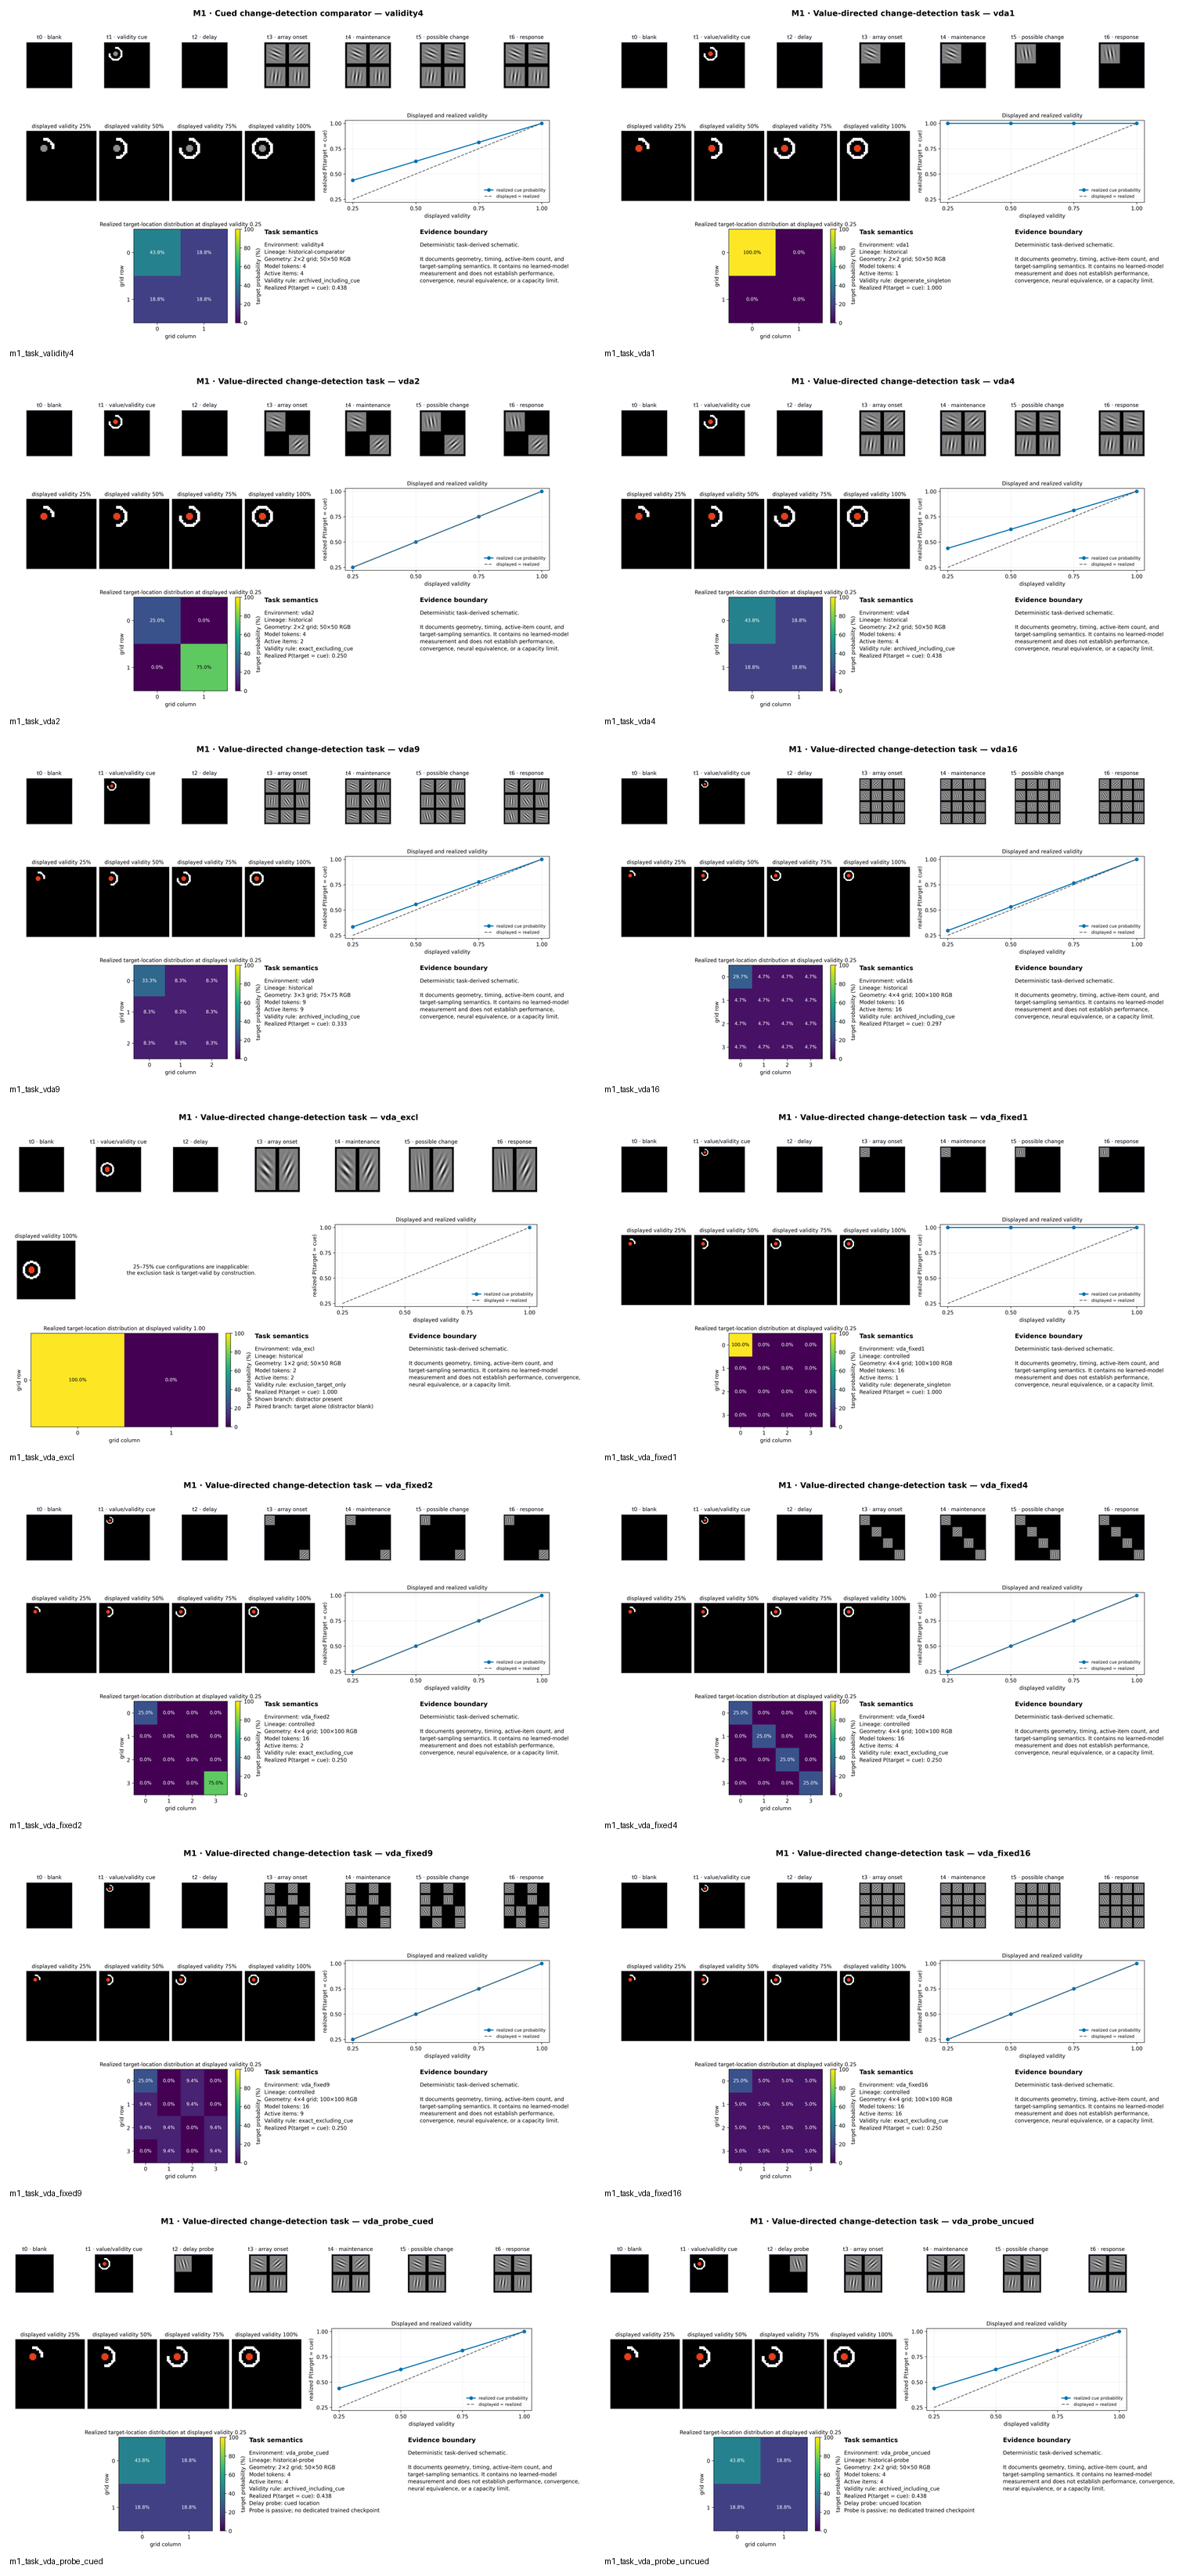
\includegraphics[width=0.72\textwidth,height=0.85\textheight,keepaspectratio]{m1_task_contact_sheet.png}
\end{center}
\captionof{figure}{All fourteen registered environments' deterministic task schematics, for cross-environment comparison. Left to right, top to bottom: neutral-validity comparator; historical VDA1/2/4/9/16; the exclusion task; cued and uncued delay probes; controlled fixed-grid VDA1/2/4/9/16.}\label{fig:m1-atlas}

\subsection{Full historical aggregate plates}\label{app:m3-full}
The eight plates behind Figure~\ref{fig:m3-overview}, regenerated from the preserved aggregate archive (checkpoints not rerun). VDA1's uncued-location panels (B, C, E, F) are omitted because a singleton has no uncued comparator.

\begin{center}
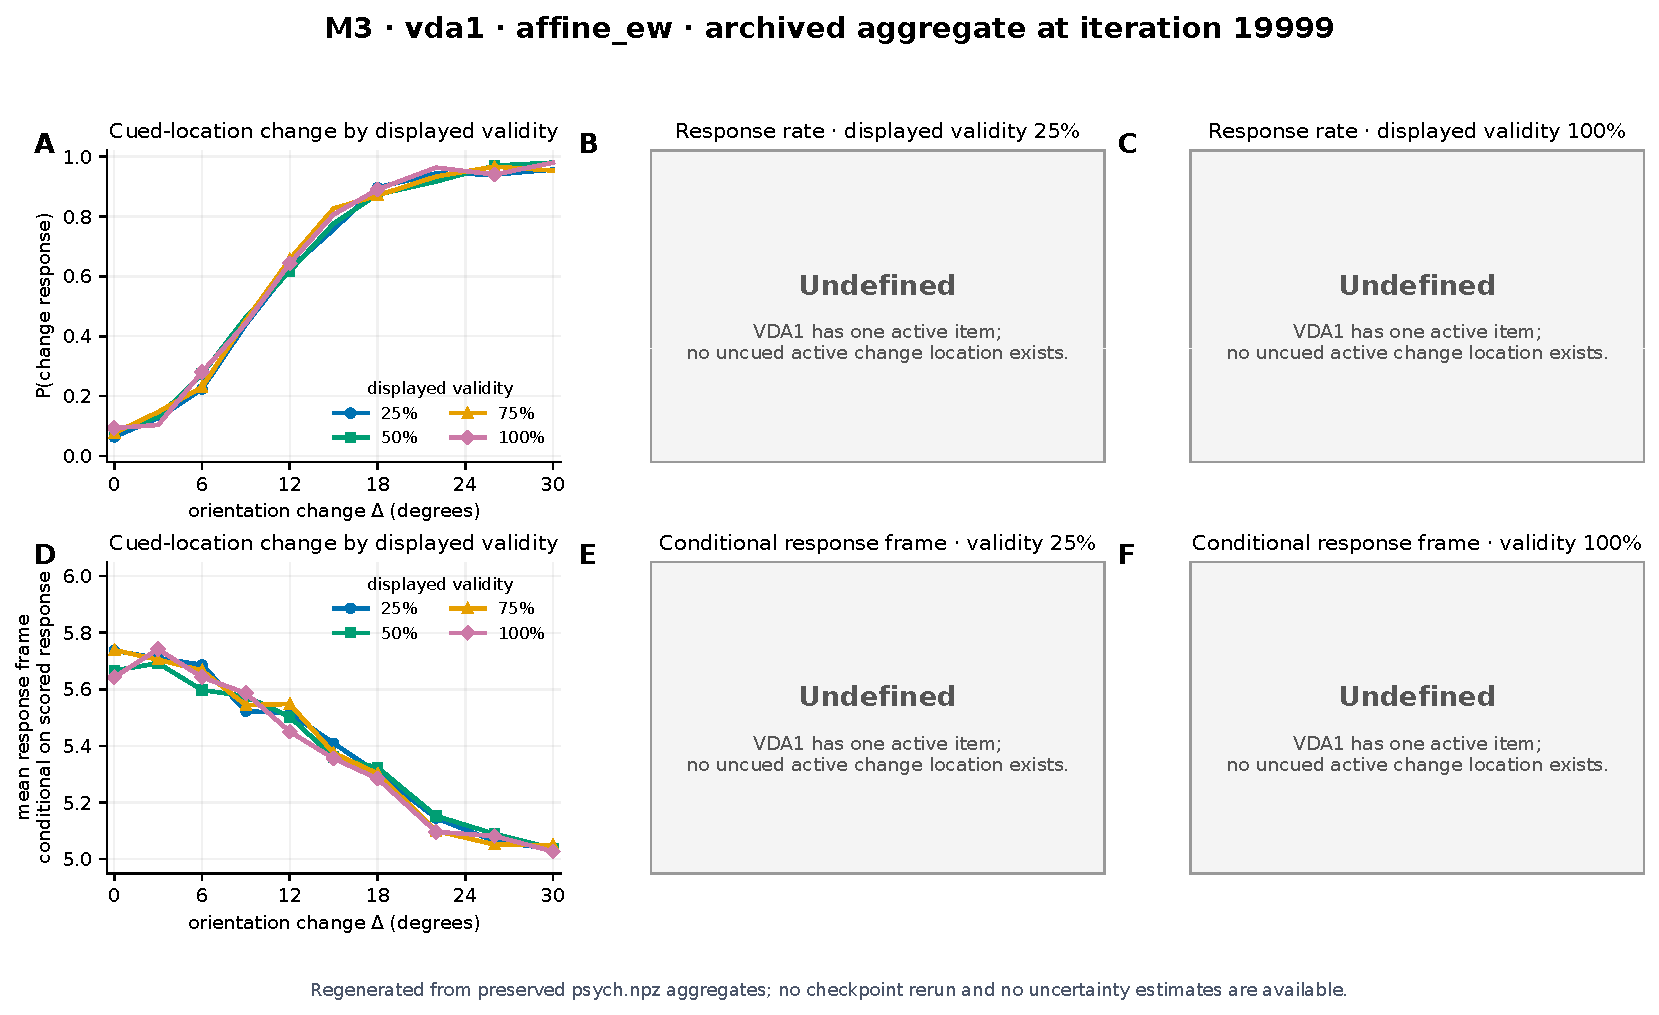
\includegraphics[width=0.44\textwidth]{m3_behavior_vda1_affine_ew.pdf}\hfill
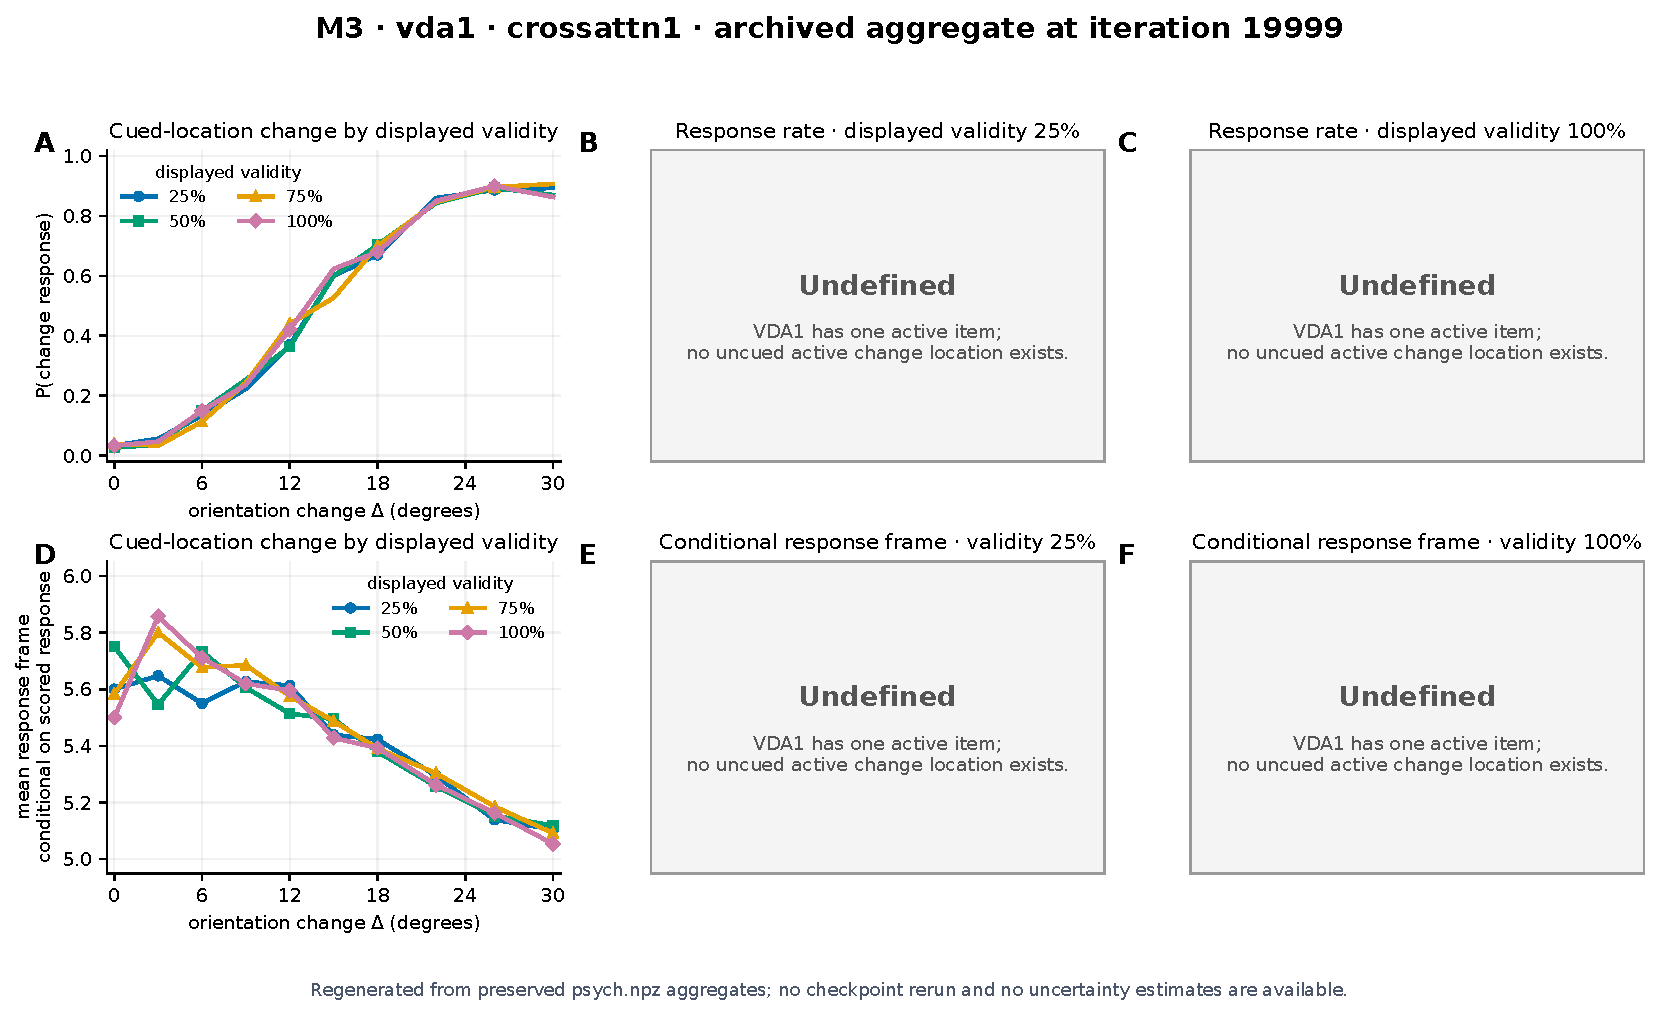
\includegraphics[width=0.44\textwidth]{m3_behavior_vda1_crossattn1.pdf}\\[3pt]
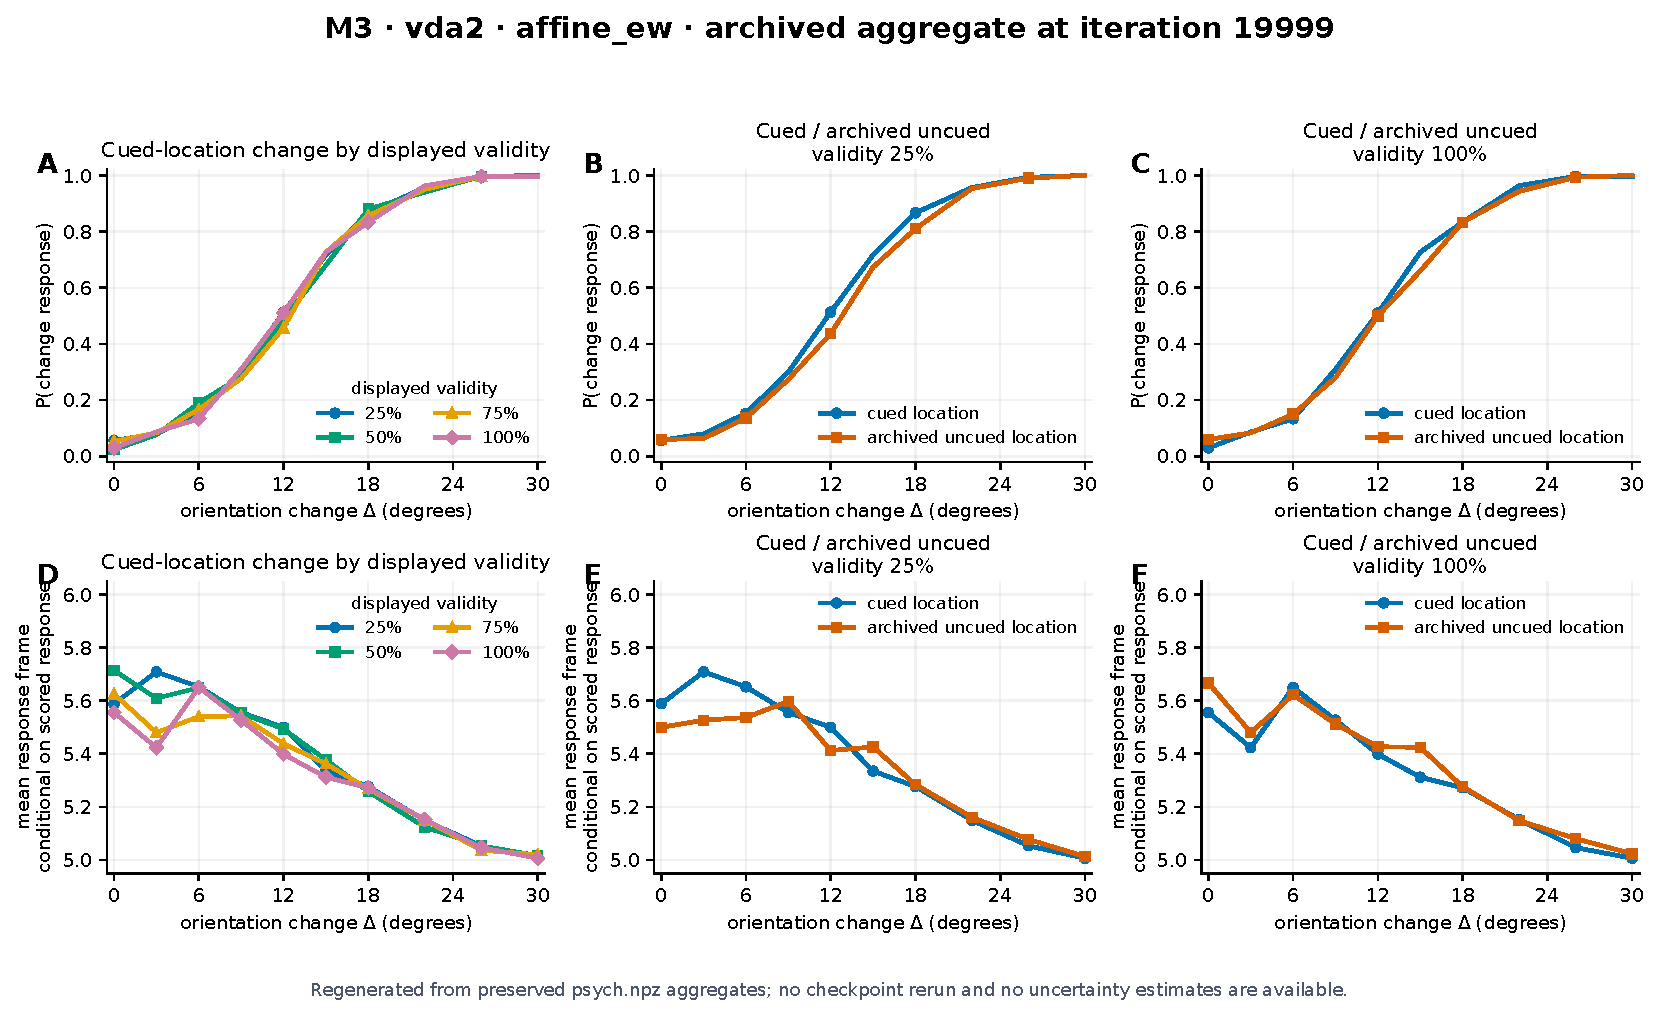
\includegraphics[width=0.44\textwidth]{m3_behavior_vda2_affine_ew.pdf}\hfill
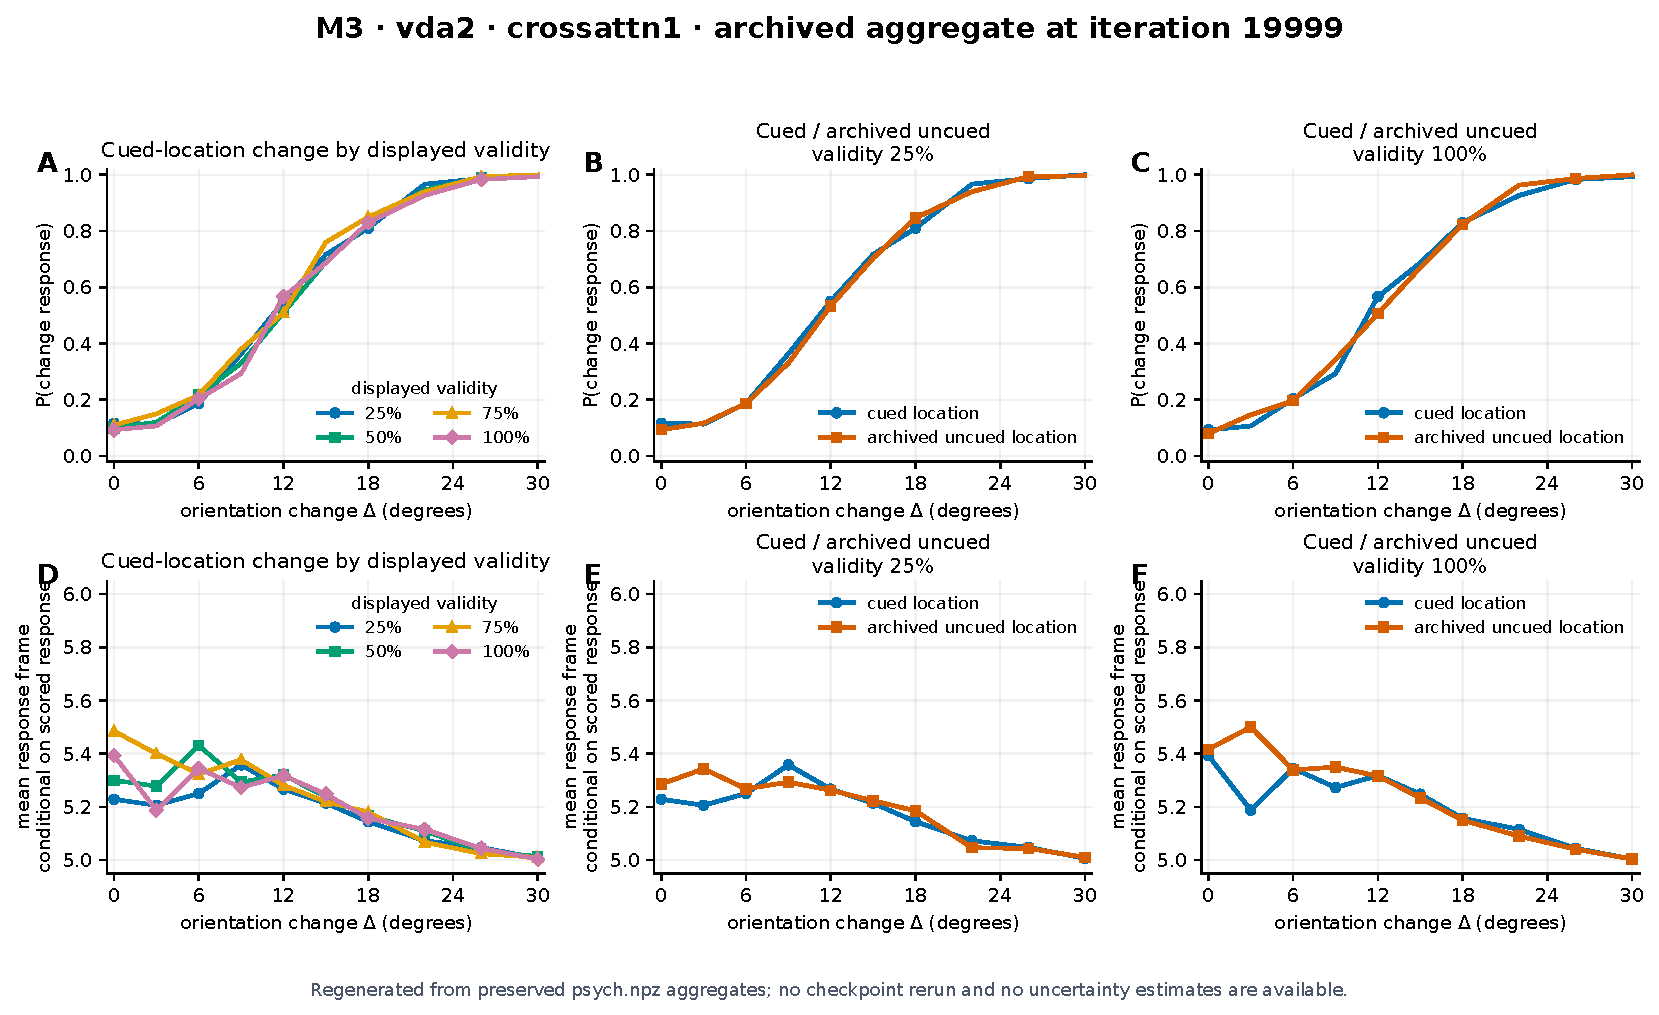
\includegraphics[width=0.44\textwidth]{m3_behavior_vda2_crossattn1.pdf}\\[3pt]
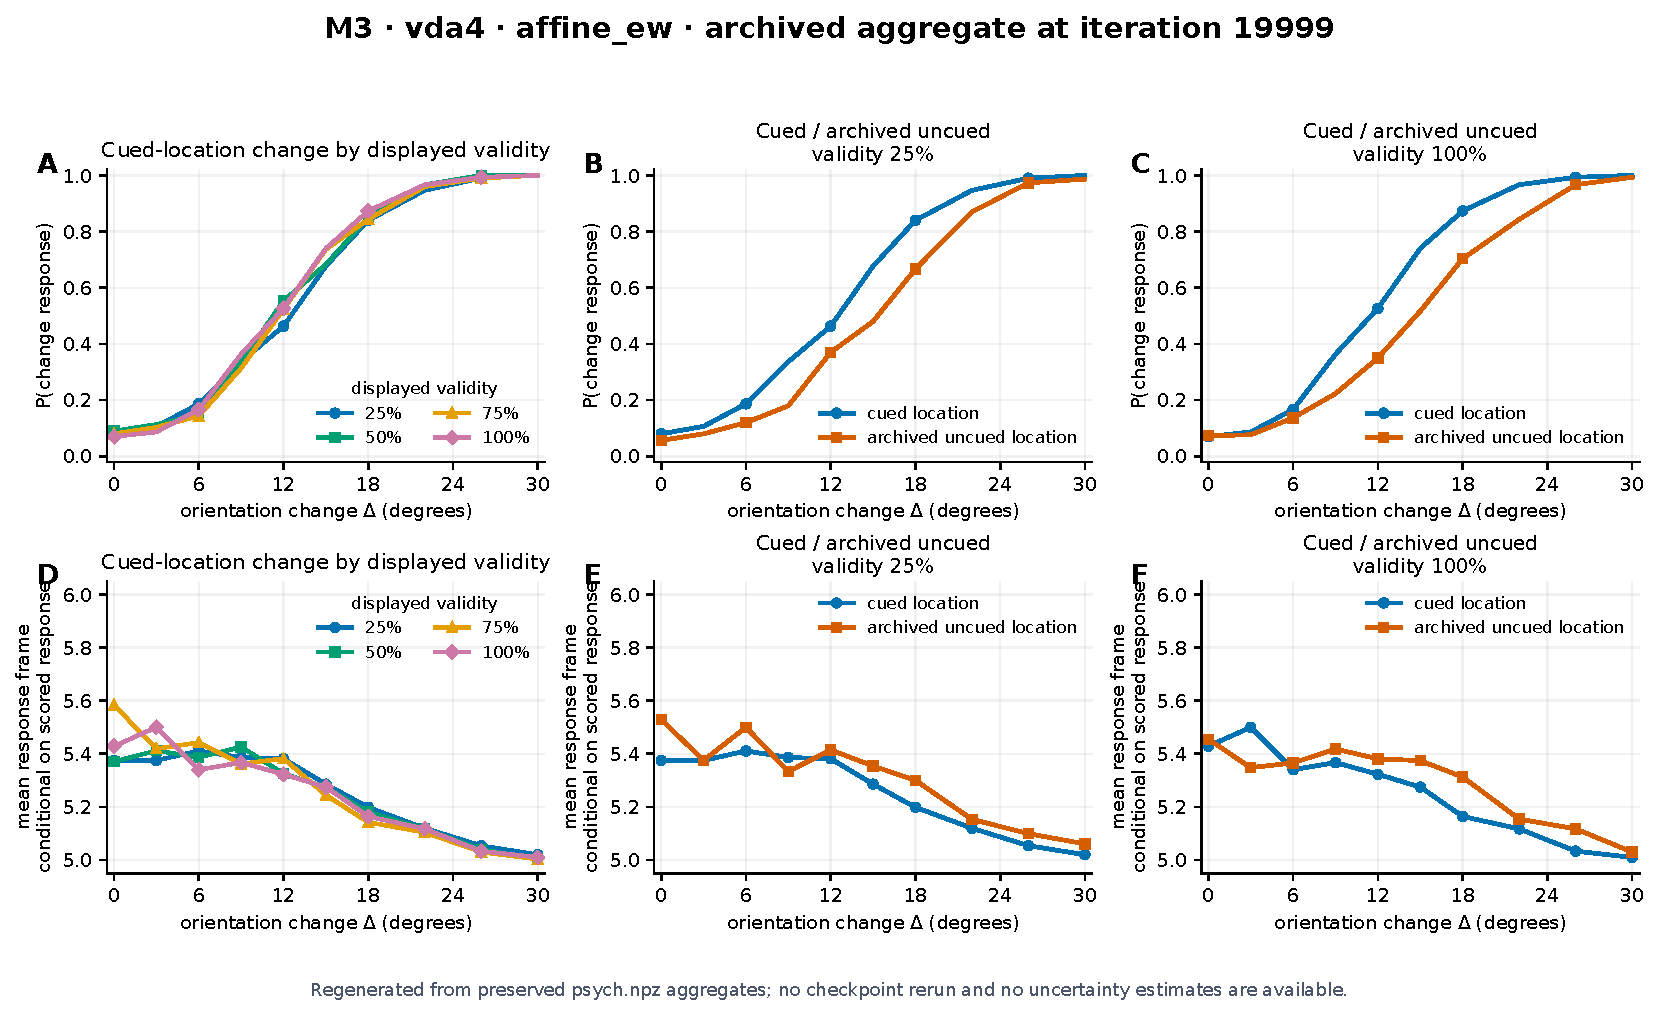
\includegraphics[width=0.44\textwidth]{m3_behavior_vda4_affine_ew.pdf}\hfill
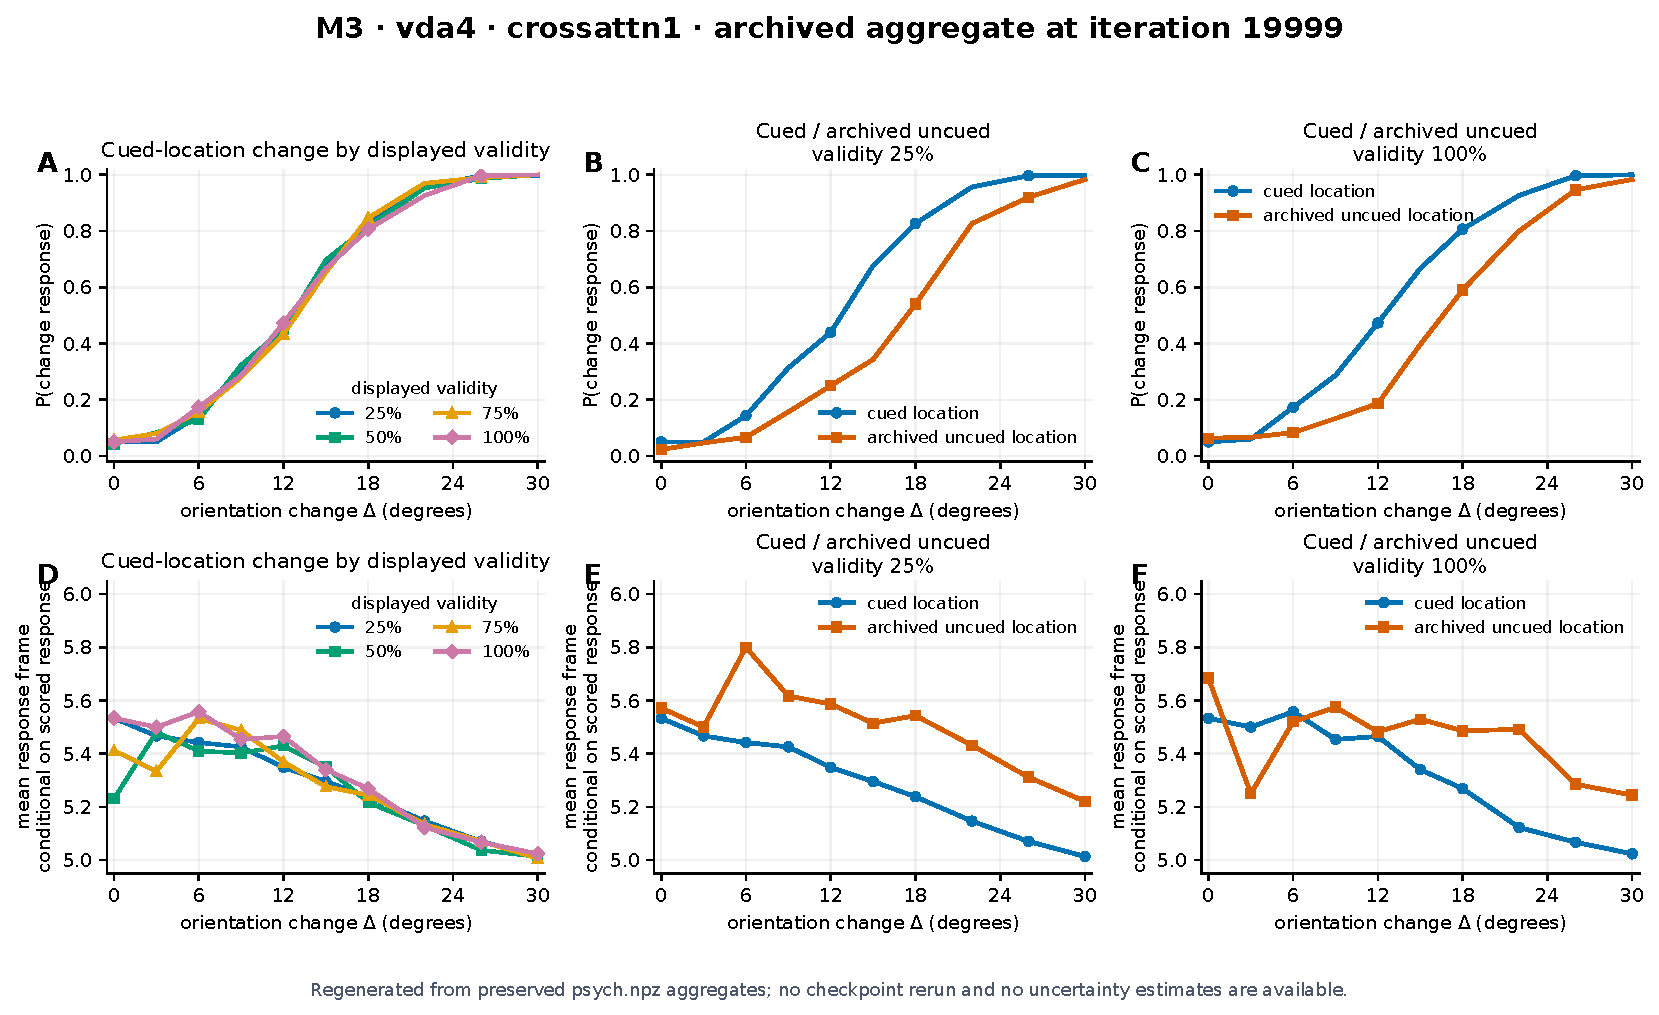
\includegraphics[width=0.44\textwidth]{m3_behavior_vda4_crossattn1.pdf}\\[3pt]
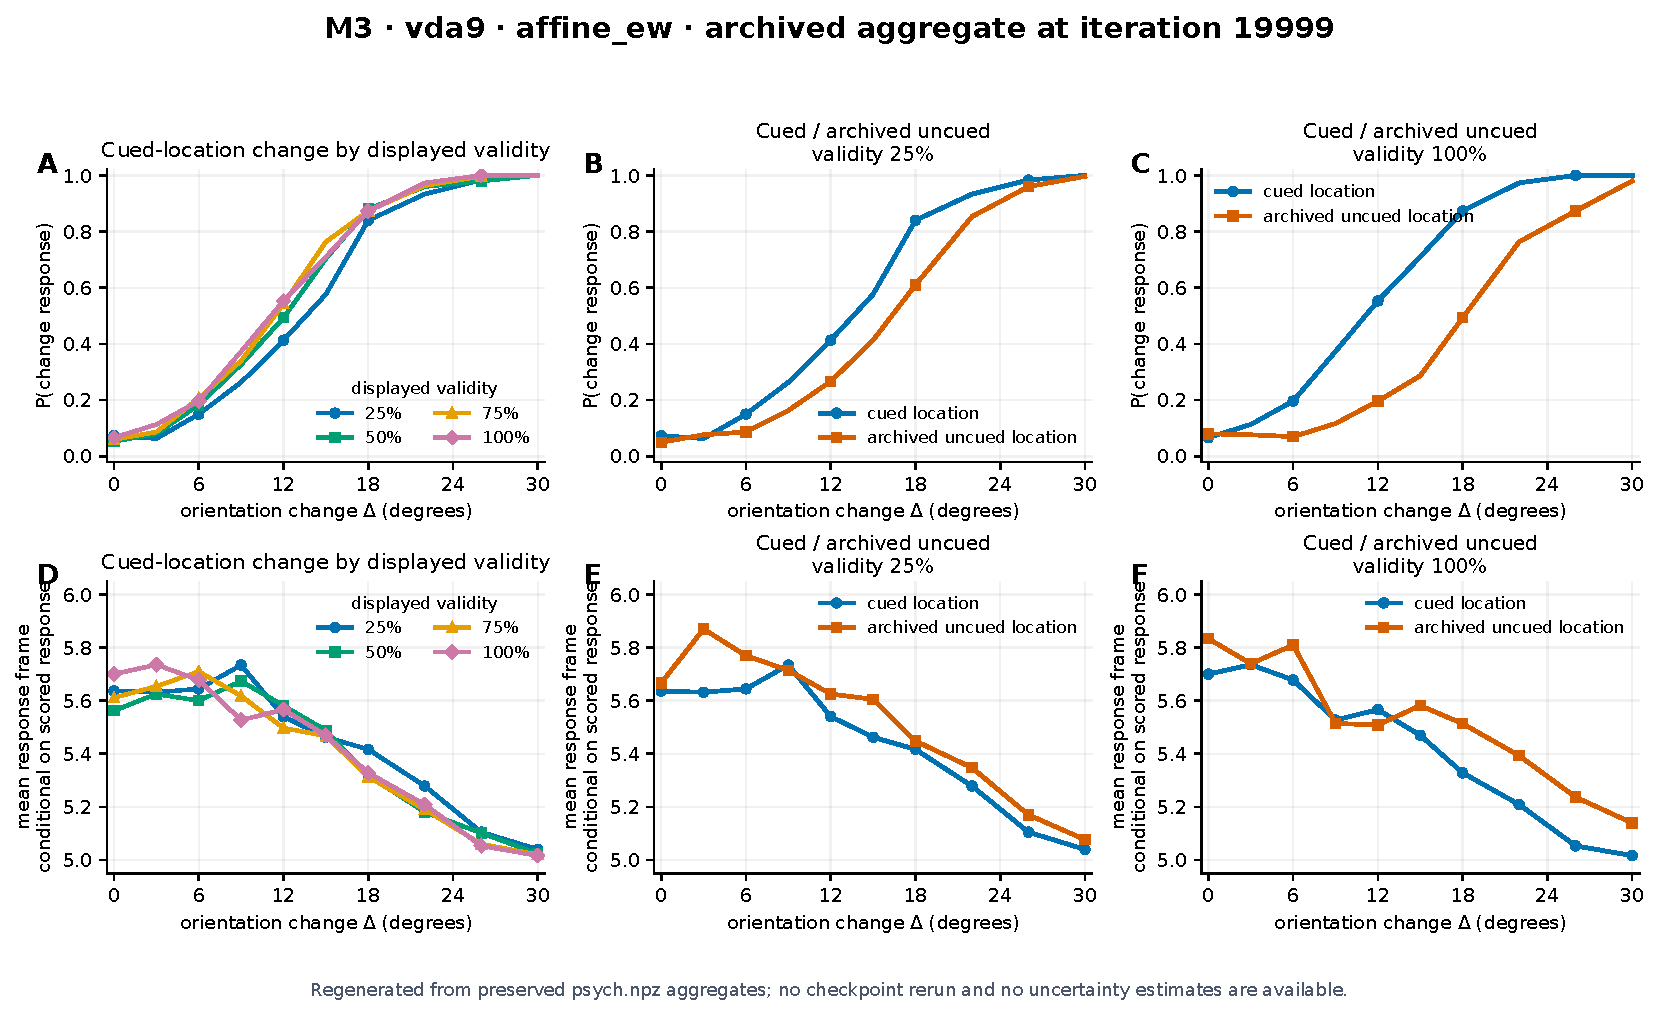
\includegraphics[width=0.44\textwidth]{m3_behavior_vda9_affine_ew.pdf}\hfill
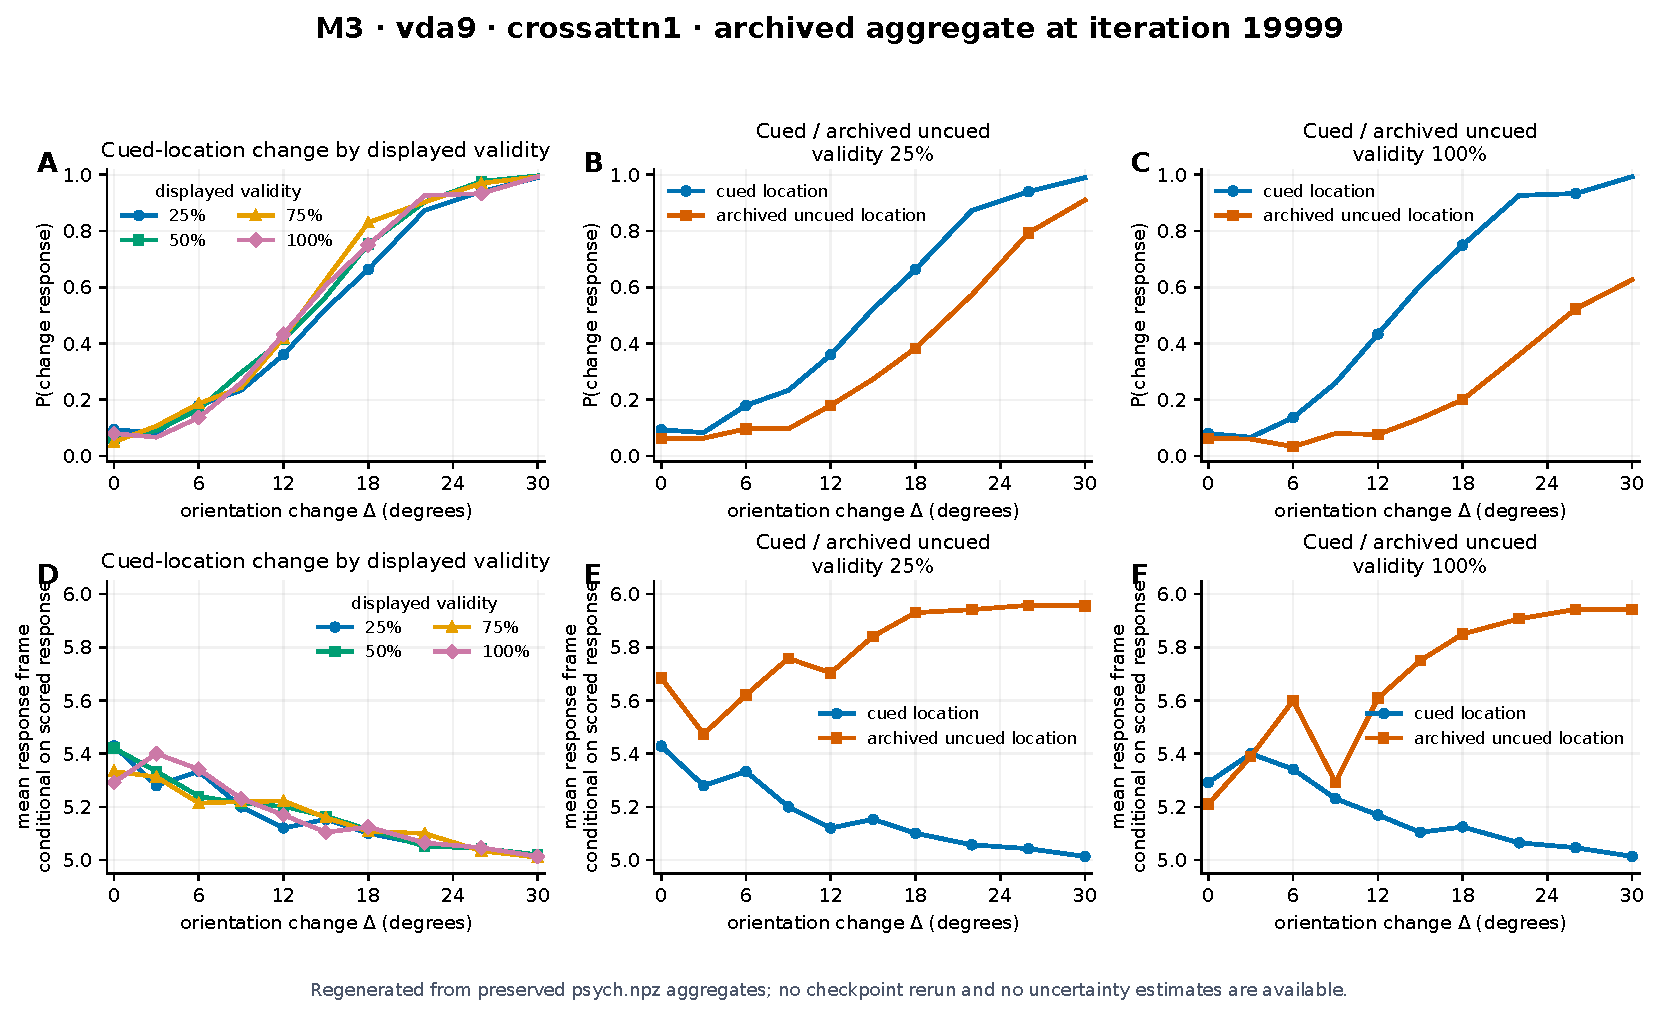
\includegraphics[width=0.44\textwidth]{m3_behavior_vda9_crossattn1.pdf}
\end{center}
\captionof{figure}{Rows: VDA1, VDA2, VDA4, VDA9. Columns: affine, cross-attention. Each panel labeled with its own routing family and environment in-figure.}

\subsection{Coverage counts by source object}\label{app:coverage}
\begin{tabular}{@{}lrr@{}}
\toprule
Status & Cells & Share \\
\midrule
Complete & 118 & 12.4\% \\
Partial & 79 & 8.3\% \\
Available & 149 & 15.7\% \\
Training & 45 & 4.7\% \\
Blocked & 204 & 21.4\% \\
Undefined & 71 & 7.5\% \\
Inapplicable & 286 & 30.0\% \\
\midrule
Total & 952 & 100.0\% \\
\bottomrule
\end{tabular}

\begingroup
\normalsize
\renewcommand{\arraystretch}{1.10}
\begin{longtable}{@{}lrrrrrrrr@{}}
\caption{Coverage counts by source object. Counts are panel--environment cells, not independent experiments. Status codes are C complete, P partial, A available, T training, B blocked, U undefined, and I inapplicable.}\label{tab:object-counts}\\
\toprule
Object & Groups & C & P & A & T & B & U & I \\
\midrule\endfirsthead
\toprule Object & Groups & C & P & A & T & B & U & I \\ \midrule\endhead
M1 & 3 & 40 & 0 & 0 & 0 & 0 & 2 & 0 \\
M2 & 4 & 56 & 0 & 0 & 0 & 0 & 0 & 0 \\
M3 & 6 & 20 & 0 & 0 & 6 & 26 & 8 & 24 \\
M4 & 4 & 2 & 14 & 3 & 4 & 18 & 5 & 10 \\
M5 & 6 & 0 & 24 & 0 & 6 & 26 & 4 & 24 \\
S1 & 1 & 0 & 0 & 14 & 0 & 0 & 0 & 0 \\
S2 & 1 & 0 & 0 & 14 & 0 & 0 & 0 & 0 \\
S3 & 1 & 0 & 0 & 14 & 0 & 0 & 0 & 0 \\
S4 & 1 & 0 & 0 & 14 & 0 & 0 & 0 & 0 \\
S5 & 2 & 0 & 0 & 0 & 0 & 0 & 0 & 28 \\
S6 & 2 & 0 & 0 & 0 & 0 & 0 & 0 & 28 \\
S7 & 2 & 0 & 0 & 0 & 0 & 0 & 0 & 28 \\
S8 & 1 & 0 & 2 & 3 & 1 & 5 & 3 & 0 \\
S9 & 1 & 0 & 2 & 0 & 1 & 8 & 3 & 0 \\
S10 & 1 & 0 & 2 & 5 & 1 & 6 & 0 & 0 \\
S11 & 2 & 0 & 4 & 8 & 2 & 11 & 3 & 0 \\
S12 & 1 & 0 & 2 & 5 & 1 & 6 & 0 & 0 \\
S13 & 5 & 0 & 5 & 27 & 5 & 20 & 13 & 0 \\
S14 & 3 & 0 & 3 & 18 & 3 & 18 & 0 & 0 \\
S15 & 9 & 0 & 9 & 18 & 9 & 36 & 18 & 36 \\
S16 & 6 & 0 & 12 & 6 & 6 & 24 & 12 & 24 \\
S17 & 6 & 0 & 0 & 0 & 0 & 0 & 0 & 84 \\
\bottomrule
\end{longtable}
\endgroup


\subsection{Exact panel--environment disposition matrix}\label{app:disposition}
Val4=\env{validity4}; H1/H2/H4/H9/H16=historical VDA set sizes; Excl=\env{vda\_excl}; PC/PU=cued/uncued probes; F1/F2/F4/F9/F16=controlled fixed-grid set sizes. C~complete, P~partial, A~available, T~training, B~blocked, U~undefined, I~inapplicable.
\newgeometry{margin=0.2in}
\begingroup
\footnotesize
\setlength{\tabcolsep}{2.5pt}
\renewcommand{\arraystretch}{1.08}
\begin{longtable}{@{}p{1.8cm}p{3.9cm}p{2.2cm}p{2.2cm}p{2.0cm}p{2.3cm}p{2.35cm}p{2.5cm}@{}}
\caption{Exact source-panel disposition by environment. The table is generated directly from \texttt{PANEL\_COVERAGE.csv}; comma-separated abbreviations name every environment assigned to each state.}\label{tab:panel-matrix}\\
\toprule
Panel & Purpose & C/P & Available & Training & Blocked & Undefined & Inapplicable \\
\midrule
\endfirsthead
\multicolumn{8}{c}{\tablename\ \thetable\ (continued)}\\
\toprule
Panel & Purpose & C/P & Available & Training & Blocked & Undefined & Inapplicable \\
\midrule
\endhead
\midrule \multicolumn{8}{r}{Continued on next page}\\ \endfoot
\bottomrule \endlastfoot
M1a & trial sequence & C: Val4, H1, H2, H4, H9, H16, Excl, PC, PU, F1, F2, F4, F9, F16 & \textemdash & \textemdash & \textemdash & \textemdash & \textemdash \\
M1b & cue/value configurations & C: Val4, H1, H2, H4, H9, H16, Excl, PC, PU, F1, F2, F4, F9, F16 & \textemdash & \textemdash & \textemdash & \textemdash & \textemdash \\
M1c & cued versus opposing change examples & C: Val4, H2, H4, H9, H16, Excl, PC, PU, F2, F4, F9, F16 & \textemdash & \textemdash & \textemdash & H1, F1 & \textemdash \\
\addlinespace[2pt]
M2a & patching and visual features & C: Val4, H1, H2, H4, H9, H16, Excl, PC, PU, F1, F2, F4, F9, F16 & \textemdash & \textemdash & \textemdash & \textemdash & \textemdash \\
M2b & routing/allocation mechanism & C: Val4, H1, H2, H4, H9, H16, Excl, PC, PU, F1, F2, F4, F9, F16 & \textemdash & \textemdash & \textemdash & \textemdash & \textemdash \\
M2c & recurrent memory update & C: Val4, H1, H2, H4, H9, H16, Excl, PC, PU, F1, F2, F4, F9, F16 & \textemdash & \textemdash & \textemdash & \textemdash & \textemdash \\
M2d & actor/critic temporal loop & C: Val4, H1, H2, H4, H9, H16, Excl, PC, PU, F1, F2, F4, F9, F16 & \textemdash & \textemdash & \textemdash & \textemdash & \textemdash \\
\addlinespace[2pt]
M3A & response rate by cue validity & C: H1, H2, H4, H9 & \textemdash & F16 & H16, F1, F2, F4, F9 & \textemdash & Val4, Excl, PC, PU \\
M3D & conditional logical response frame by displayed validity & C: H1, H2, H4, H9 & \textemdash & F16 & H16, F1, F2, F4, F9 & \textemdash & Val4, Excl, PC, PU \\
M3B & change-response probability: cued versus archived uncued, low displayed validity & C: H2, H4, H9 & \textemdash & F16 & H16, F2, F4, F9 & H1, F1 & Val4, Excl, PC, PU \\
M3C & change-response probability: cued versus archived uncued, high displayed validity & C: H2, H4, H9 & \textemdash & F16 & H16, F2, F4, F9 & H1, F1 & Val4, Excl, PC, PU \\
M3E & conditional logical response frame: cued versus archived uncued, low displayed validity & C: H2, H4, H9 & \textemdash & F16 & H16, F2, F4, F9 & H1, F1 & Val4, Excl, PC, PU \\
M3F & conditional logical response frame: cued versus archived uncued, high displayed validity & C: H2, H4, H9 & \textemdash & F16 & H16, F2, F4, F9 & H1, F1 & Val4, Excl, PC, PU \\
\addlinespace[2pt]
M4A & allocation maps by cue validity and time & P: H1, H2, H4, H9 & \textemdash & F16 & H16, F1, F2, F4, F9 & \textemdash & Val4, Excl, PC, PU \\
M4B & S1 allocation at change time for S1 changes & C: H4, H9; P: H1, H2, Excl & Val4 & F16 & H16, F1, F2, F4, F9 & \textemdash & PC, PU \\
M4C & S1 allocation when another location changes & P: H2, H4, H9 & Val4 & F16 & H16, F2, F4, F9 & H1, Excl, F1 & PC, PU \\
M4D & S1/S4 allocation over trial time & P: H2, H4, H9, Excl & Val4 & F16 & H16, F2, F4, F9 & H1, F1 & PC, PU \\
\addlinespace[2pt]
M5A & response rate: natural/target intervention & P: H1, H2, H4, H9 & \textemdash & F16 & H16, F1, F2, F4, F9 & \textemdash & Val4, Excl, PC, PU \\
M5B & response rate: matched-location intervention contrast & P: H1, H2, H4, H9 & \textemdash & F16 & H16, F2, F4, F9 & F1 & Val4, Excl, PC, PU \\
M5C & response rate: competing-location intervention contrast & P: H1, H2, H4, H9 & \textemdash & F16 & H16, F2, F4, F9 & F1 & Val4, Excl, PC, PU \\
M5D & reaction time: natural/target intervention & P: H1, H2, H4, H9 & \textemdash & F16 & H16, F1, F2, F4, F9 & \textemdash & Val4, Excl, PC, PU \\
M5E & reaction time: matched-location intervention contrast & P: H1, H2, H4, H9 & \textemdash & F16 & H16, F2, F4, F9 & F1 & Val4, Excl, PC, PU \\
M5F & reaction time: competing-location intervention contrast & P: H1, H2, H4, H9 & \textemdash & F16 & H16, F2, F4, F9 & F1 & Val4, Excl, PC, PU \\
\addlinespace[2pt]
S1 & high-level recurrent circuit & \textemdash & Val4, H1, H2, H4, H9, H16, Excl, PC, PU, F1, F2, F4, F9, F16 & \textemdash & \textemdash & \textemdash & \textemdash \\
\addlinespace[2pt]
S2 & patch-wise recurrent memory & \textemdash & Val4, H1, H2, H4, H9, H16, Excl, PC, PU, F1, F2, F4, F9, F16 & \textemdash & \textemdash & \textemdash & \textemdash \\
\addlinespace[2pt]
S3 & immediate-input allocation before memory & \textemdash & Val4, H1, H2, H4, H9, H16, Excl, PC, PU, F1, F2, F4, F9, F16 & \textemdash & \textemdash & \textemdash & \textemdash \\
\addlinespace[2pt]
S4 & memory feedback into allocation & \textemdash & Val4, H1, H2, H4, H9, H16, Excl, PC, PU, F1, F2, F4, F9, F16 & \textemdash & \textemdash & \textemdash & \textemdash \\
\addlinespace[2pt]
S5a & memory-token architecture & \textemdash & \textemdash & \textemdash & \textemdash & \textemdash & Val4, H1, H2, H4, H9, H16, Excl, PC, PU, F1, F2, F4, F9, F16 \\
S5b-e & memory-token behavior/allocation battery & \textemdash & \textemdash & \textemdash & \textemdash & \textemdash & Val4, H1, H2, H4, H9, H16, Excl, PC, PU, F1, F2, F4, F9, F16 \\
\addlinespace[2pt]
S6a & additive Q/K/V architecture & \textemdash & \textemdash & \textemdash & \textemdash & \textemdash & Val4, H1, H2, H4, H9, H16, Excl, PC, PU, F1, F2, F4, F9, F16 \\
S6b-e & additive Q/K/V behavior/allocation battery & \textemdash & \textemdash & \textemdash & \textemdash & \textemdash & Val4, H1, H2, H4, H9, H16, Excl, PC, PU, F1, F2, F4, F9, F16 \\
\addlinespace[2pt]
S7a & multiplicative Q/K/V architecture & \textemdash & \textemdash & \textemdash & \textemdash & \textemdash & Val4, H1, H2, H4, H9, H16, Excl, PC, PU, F1, F2, F4, F9, F16 \\
S7b-e & multiplicative Q/K/V behavior/allocation battery & \textemdash & \textemdash & \textemdash & \textemdash & \textemdash & Val4, H1, H2, H4, H9, H16, Excl, PC, PU, F1, F2, F4, F9, F16 \\
\addlinespace[2pt]
S8-all & all-slot change-location decoding, natural/max allocation, t5/t6 & P: H4, H9 & Val4, PC, PU & F16 & H2, H16, F2, F4, F9 & H1, Excl, F1 & \textemdash \\
\addlinespace[2pt]
S9-all & all-slot location decoding across four allocation conditions & P: H4, H9 & \textemdash & F16 & Val4, H2, H16, PC, PU, F2, F4, F9 & H1, Excl, F1 & \textemdash \\
\addlinespace[2pt]
S10-all & single-slot binary change decoding across allocation conditions & P: H4, H9 & Val4, H1, Excl, PC, PU & F16 & H2, H16, F1, F2, F4, F9 & \textemdash & \textemdash \\
\addlinespace[2pt]
S11-location & actor-layer change-location decoding & P: H4, H9 & Val4, PC, PU & F16 & H2, H16, F2, F4, F9 & H1, Excl, F1 & \textemdash \\
S11-binary & actor-layer binary change decoding & P: H4, H9 & Val4, H1, Excl, PC, PU & F16 & H2, H16, F1, F2, F4, F9 & \textemdash & \textemdash \\
\addlinespace[2pt]
S12-all & graded actor-layer binary decoding under S1 inhibition & P: H4, H9 & Val4, H1, Excl, PC, PU & F16 & H2, H16, F1, F2, F4, F9 & \textemdash & \textemdash \\
\addlinespace[2pt]
S13-all & all-trial Wait/Declare logit scatter and density & P: H9 & Val4, H1, H2, H4, Excl, PC, PU & F16 & H16, F1, F2, F4, F9 & \textemdash & \textemdash \\
S13-S1 & Wait/Declare logit scatter and density for S1 changes & P: H9 & Val4, H1, H2, H4, Excl, PC, PU & F16 & H16, F1, F2, F4, F9 & \textemdash & \textemdash \\
S13-S2 & Wait/Declare logit scatter and density for S2 changes & P: H9 & Val4, H2, H4, PC, PU & F16 & H16, F2, F4, F9 & H1, Excl, F1 & \textemdash \\
S13-S3 & Wait/Declare logit scatter and density for S3 changes & P: H9 & Val4, H4, PC, PU & F16 & H16, F4, F9 & H1, H2, Excl, F1, F2 & \textemdash \\
S13-S4 & Wait/Declare logit scatter and density for S4 changes & P: H9 & Val4, H4, PC, PU & F16 & H16, F4, F9 & H1, H2, Excl, F1, F2 & \textemdash \\
\addlinespace[2pt]
S14-natural & natural S1-change logit scatter/density & P: H9 & Val4, H1, H4, Excl, PC, PU & F16 & H2, H16, F1, F2, F4, F9 & \textemdash & \textemdash \\
S14-max & maximal S1 allocation logit scatter/density & P: H9 & Val4, H1, H4, Excl, PC, PU & F16 & H2, H16, F1, F2, F4, F9 & \textemdash & \textemdash \\
S14-zero & zero S1 allocation logit scatter/density & P: H9 & Val4, H1, H4, Excl, PC, PU & F16 & H2, H16, F1, F2, F4, F9 & \textemdash & \textemdash \\
\addlinespace[2pt]
S15A & TD error by cue/change location & P: H9 & H2, H4 & F16 & H16, F2, F4, F9 & H1, F1 & Val4, Excl, PC, PU \\
S15B & TD error with target allocation clamp, low cue & P: H9 & H2, H4 & F16 & H16, F2, F4, F9 & H1, F1 & Val4, Excl, PC, PU \\
S15C & TD error with target allocation clamp, high cue & P: H9 & H2, H4 & F16 & H16, F2, F4, F9 & H1, F1 & Val4, Excl, PC, PU \\
S15D & TD error by allocation dose and location & P: H9 & H2, H4 & F16 & H16, F2, F4, F9 & H1, F1 & Val4, Excl, PC, PU \\
S15E & TD error under competing-location clamp, low cue & P: H9 & H2, H4 & F16 & H16, F2, F4, F9 & H1, F1 & Val4, Excl, PC, PU \\
S15F & TD error under competing-location clamp, high cue & P: H9 & H2, H4 & F16 & H16, F2, F4, F9 & H1, F1 & Val4, Excl, PC, PU \\
S15G & value by change magnitude with target clamp & P: H9 & H2, H4 & F16 & H16, F2, F4, F9 & H1, F1 & Val4, Excl, PC, PU \\
S15H & value by opposing-location allocation dose & P: H9 & H2, H4 & F16 & H16, F2, F4, F9 & H1, F1 & Val4, Excl, PC, PU \\
S15I & hit rate by opposing-location allocation dose & P: H9 & H2, H4 & F16 & H16, F2, F4, F9 & H1, F1 & Val4, Excl, PC, PU \\
\addlinespace[2pt]
S16A & criterion vs allocation at change & P: H4, H9 & H2 & F16 & H16, F2, F4, F9 & H1, F1 & Val4, Excl, PC, PU \\
S16B & criterion vs cue-time allocation with change-time control & P: H4, H9 & H2 & F16 & H16, F2, F4, F9 & H1, F1 & Val4, Excl, PC, PU \\
S16C & criterion vs cue-time allocation & P: H4, H9 & H2 & F16 & H16, F2, F4, F9 & H1, F1 & Val4, Excl, PC, PU \\
S16D & sensitivity vs allocation at change & P: H4, H9 & H2 & F16 & H16, F2, F4, F9 & H1, F1 & Val4, Excl, PC, PU \\
S16E & sensitivity vs cue-time allocation with change-time control & P: H4, H9 & H2 & F16 & H16, F2, F4, F9 & H1, F1 & Val4, Excl, PC, PU \\
S16F & sensitivity vs cue-time allocation & P: H4, H9 & H2 & F16 & H16, F2, F4, F9 & H1, F1 & Val4, Excl, PC, PU \\
\addlinespace[2pt]
S17-action-behavior & three behavioral rows: supervised actions & \textemdash & \textemdash & \textemdash & \textemdash & \textemdash & Val4, H1, H2, H4, H9, H16, Excl, PC, PU, F1, F2, F4, F9, F16 \\
S17-belief-behavior & three behavioral rows: supervised beliefs & \textemdash & \textemdash & \textemdash & \textemdash & \textemdash & Val4, H1, H2, H4, H9, H16, Excl, PC, PU, F1, F2, F4, F9, F16 \\
S17-rl-behavior & three behavioral rows: reinforcement learning & \textemdash & \textemdash & \textemdash & \textemdash & \textemdash & Val4, H1, H2, H4, H9, H16, Excl, PC, PU, F1, F2, F4, F9, F16 \\
S17-action-allocation & allocation row: supervised actions & \textemdash & \textemdash & \textemdash & \textemdash & \textemdash & Val4, H1, H2, H4, H9, H16, Excl, PC, PU, F1, F2, F4, F9, F16 \\
S17-belief-allocation & allocation row: supervised beliefs & \textemdash & \textemdash & \textemdash & \textemdash & \textemdash & Val4, H1, H2, H4, H9, H16, Excl, PC, PU, F1, F2, F4, F9, F16 \\
S17-rl-allocation & allocation row: reinforcement learning & \textemdash & \textemdash & \textemdash & \textemdash & \textemdash & Val4, H1, H2, H4, H9, H16, Excl, PC, PU, F1, F2, F4, F9, F16 \\
\end{longtable}
\endgroup

\restoregeometry

\subsection{Matched-width constituent values}\label{app:matched-width-constituents}
Absolute and within-checkpoint values behind the d256-minus-d128 summary of Section~\ref{sec:width-behavior}, regenerated from the twelve hash-verified matched-width shards.
\begingroup\scriptsize\setlength{\tabcolsep}{2.7pt}
\captionof{table}{\textbf{Absolute valid-location response probabilities.} Checkpoint-recomputed values at displayed validity 0.75; each cell uses 300 trials. These are the constituents behind Figure~\ref{fig:matched-width}A, not replicated estimates of a width effect.}\label{tab:absolute-behavior}
\begin{center}
\begin{tabular}{@{}llr*{10}{r}@{}}
\toprule
Task & Routing & Width & \multicolumn{10}{c}{Orientation change (degrees)} \\
\cmidrule(lr){4-13}
 & & & 2 & 6 & 10 & 14 & 18 & 22 & 26 & 30 & 34 & 38 \\ 
\midrule
VDA1 & \texttt{affine} & 128 & 0.133 & 0.250 & 0.460 & 0.697 & 0.903 & 0.923 & 0.960 & 0.957 & 0.953 & 0.947 \\
VDA1 & \texttt{affine} & 256 & 0.123 & 0.230 & 0.487 & 0.653 & 0.907 & 0.917 & 0.953 & 0.953 & 0.947 & 0.963 \\
VDA1 & \texttt{cross-attn} & 128 & 0.060 & 0.123 & 0.313 & 0.520 & 0.717 & 0.843 & 0.863 & 0.873 & 0.890 & 0.857 \\
VDA1 & \texttt{cross-attn} & 256 & 0.177 & 0.287 & 0.480 & 0.730 & 0.810 & 0.910 & 0.897 & 0.907 & 0.923 & 0.897 \\
VDA4 & \texttt{affine} & 128 & 0.093 & 0.177 & 0.437 & 0.663 & 0.833 & 0.947 & 0.973 & 0.997 & 1.000 & 1.000 \\
VDA4 & \texttt{affine} & 256 & 0.120 & 0.337 & 0.587 & 0.777 & 0.933 & 0.980 & 0.990 & 0.997 & 0.997 & 1.000 \\
VDA4 & \texttt{cross-attn} & 128 & 0.063 & 0.140 & 0.410 & 0.617 & 0.803 & 0.967 & 0.980 & 1.000 & 1.000 & 1.000 \\
VDA4 & \texttt{cross-attn} & 256 & 0.037 & 0.113 & 0.303 & 0.487 & 0.690 & 0.923 & 0.953 & 0.993 & 1.000 & 1.000 \\
VDA9 & \texttt{affine} & 128 & 0.073 & 0.170 & 0.420 & 0.640 & 0.863 & 0.970 & 0.990 & 1.000 & 1.000 & 1.000 \\
VDA9 & \texttt{affine} & 256 & 0.087 & 0.140 & 0.407 & 0.597 & 0.813 & 0.963 & 0.983 & 0.997 & 1.000 & 1.000 \\
\bottomrule
\end{tabular}
\end{center}
\endgroup

\begingroup\scriptsize\setlength{\tabcolsep}{4.0pt}
\captionof{table}{\textbf{Within-checkpoint clamp constituents.} Each entry is $D_{w,x}(b)=d'_{w,x}(b)-d'_{w,x}(0)$ from 250 trials per bias, condition, and checkpoint. VDA1 invalid-location effects are undefined and therefore absent. Figure~\ref{fig:matched-width}C--D plots $W_x(b)=D_{256,x}(b)-D_{128,x}(b)$.}\label{tab:clamp-constituents}
\begin{center}
\begin{tabular}{@{}llll*{5}{r}@{}}
\toprule
Task & Routing & Condition & Width & \multicolumn{5}{c}{Assigned key-logit bias $b$} \\
\cmidrule(lr){5-9}
 & & & & -6 & -3 & 0 & 3 & 6 \\ 
\midrule
VDA1 & \texttt{affine} & valid & 128 & -1.681 & -1.124 & 0.000 & -0.474 & -0.572 \\
VDA1 & \texttt{affine} & valid & 256 & -0.017 & -0.017 & 0.000 & -0.017 & -0.020 \\
VDA1 & \texttt{cross-attn} & valid & 128 & -0.470 & 0.054 & 0.000 & 0.071 & 0.137 \\
VDA1 & \texttt{cross-attn} & valid & 256 & 0.087 & 0.028 & 0.000 & -0.019 & -0.102 \\
VDA4 & \texttt{affine} & valid & 128 & -1.384 & -0.622 & 0.000 & 0.247 & 0.092 \\
VDA4 & \texttt{affine} & invalid & 128 & 0.375 & 0.351 & 0.000 & -0.785 & -1.484 \\
VDA4 & \texttt{affine} & valid & 256 & -0.491 & -0.176 & 0.000 & 0.046 & -0.156 \\
VDA4 & \texttt{affine} & invalid & 256 & 0.284 & 0.146 & 0.000 & -0.377 & -0.787 \\
VDA4 & \texttt{cross-attn} & valid & 128 & -0.544 & -0.426 & 0.000 & -0.297 & -0.456 \\
VDA4 & \texttt{cross-attn} & invalid & 128 & 0.172 & 0.172 & 0.000 & -0.610 & -0.750 \\
VDA4 & \texttt{cross-attn} & valid & 256 & -0.736 & -0.577 & 0.000 & -0.009 & -0.047 \\
VDA4 & \texttt{cross-attn} & invalid & 256 & 0.117 & 0.133 & 0.000 & -0.434 & -0.574 \\
VDA9 & \texttt{affine} & valid & 128 & -0.978 & -0.300 & 0.000 & -0.097 & -0.199 \\
VDA9 & \texttt{affine} & invalid & 128 & 0.420 & 0.391 & 0.000 & -0.187 & -0.462 \\
VDA9 & \texttt{affine} & valid & 256 & -0.046 & 0.040 & 0.000 & 0.086 & 0.097 \\
VDA9 & \texttt{affine} & invalid & 256 & 0.150 & 0.076 & 0.000 & -0.160 & -0.378 \\
\bottomrule
\end{tabular}
\end{center}
\endgroup


\subsection{Artifact locations and provenance}\label{app:provenance}
\small
\begin{longtable}{@{}p{3.4cm} p{7.5cm} p{5.5cm}@{}}
\toprule
Artifact & Path & Provenance\\
\midrule\endhead
This manuscript & \path{reports/vda_series/manuscript/VDA_Set_Size.pdf} & Narrative manuscript, 2026-07-20\\
M1 task products & \path{reports/vda_series/figures/task/} & Regenerated deterministic specifications\\
M2 architecture & \path{reports/vda_series/figures/architecture/} & Source-derived specification diagrams\\
M3 behavior & \path{reports/vda_series/figures/behavior/} & Regenerated from preserved aggregate NPZ\\
First-wave checkpoint products & \path{reports/vda_series/figures/first_wave/} & Byte-identical snapshots, approved 96/300 production build\\
Matched-width snapshots & \path{reports/vda_series/figures/matched_width/} & Projection from the audited v15 summary\\
VDA16 cross-attention shard & \path{RViT_plus_paper_jepa_grid9/reports/vda_series/vda16_crossattn_nodecay_20260719_production/} & Terminal, validation-gated controlled evidence\\
VDA16 affine shard & \path{RViT_plus_paper_jepa_grid9/reports/vda_series/vda16_affine_nodecay_20260720_production/} & Terminal, validation-gated; freezes the cross-attention companion shard\\
VDA16 paired-location experiment & \path{RViT_plus_paper_jepa_grid9/reports/vda_series/vda16_cued_vs_opposite_attention_20260719/} & Checkpoint-rerun trial cache and hash manifest\\
Change-location intervention & \path{RViT_plus_paper_jepa_grid9/reports/vda_series/change_location_intervention_20260719/} & Checkpoint-recomputed; VDA4/VDA9 recorded blocked\\
Logistic-fit re-analysis & \path{reports/vda_series/figures/psychometric_fits/} & Re-analysis of cached arrays; no checkpoint access\\
Memory-decay comparison & \path{RViT_plus_paper_jepa_grid9/analysis/vda4_decay_comparison.py} & Checkpoint-recomputed, paired frozen checkpoints\\
Panel inventory / coverage matrix & \path{reports/vda_series/MAH_SOURCE_PANEL_INVENTORY.md}, \path{PANEL_COVERAGE.csv} & Source-grounded inventory and machine-readable disposition matrix\\
\bottomrule
\end{longtable}
\twocolumn

\end{document}

